\documentclass[11pt]{amsart}
\pdfgentounicode=1
\pdfglyphtounicode{parenleftbig}{0028}
\pdfglyphtounicode{parenrightbig}{0029}
\pdfglyphtounicode{bracketleftbig}{005B}
\pdfglyphtounicode{bracketrightbig}{005D}
\pdfglyphtounicode{ceilingleftbig}{2308}
\pdfglyphtounicode{ceilingrightbig}{2309}
\pdfglyphtounicode{vextendsingle}{007C}
\pdfglyphtounicode{parenleftbigg}{0028}
\pdfglyphtounicode{parenrightbigg}{0029}
\pdfglyphtounicode{circleplustext}{2A01}
\pdfglyphtounicode{circleplusdisplay}{2A01}
\pdfglyphtounicode{summationtext}{2211}
\pdfglyphtounicode{producttext}{220F}
\pdfglyphtounicode{logicalandtext}{22C0}
\pdfglyphtounicode{summationdisplay}{2211}
\pdfglyphtounicode{productdisplay}{220F}
\pdfglyphtounicode{uniondisplay}{22C3}
\pdfglyphtounicode{hatwide}{0302}
\pdfglyphtounicode{hatwider}{0302}
\pdfglyphtounicode{tildewide}{0303}
\pdfglyphtounicode{mapsto}{007C}
\pdfglyphtounicode{axisshort}{002D}
\pdfglyphtounicode{arrowaxisright}{2192}
\usepackage{amsmath,amssymb,amsthm}
\newcommand{\mathscr}{\mathcal}
\usepackage{mathtools,microtype,enumitem,booktabs,graphicx}
\usepackage{tikz}
\usetikzlibrary{arrows.meta,positioning}
\usepackage[hidelinks,unicode,hypertexnames=false,bookmarksdepth=2]{hyperref}
\hypersetup{pdftitle={Minimal models and Mori fibre spaces for generalized log canonical Q-pairs},
 pdfauthor={OpenAI},pdfsubject={Existence of minimal models and Mori fibre spaces with fixed rational nef data}}
\usepackage[capitalise,nameinlink,noabbrev]{cleveref}
\setlength{\textwidth}{6.45in}
\setlength{\oddsidemargin}{0.025in}
\setlength{\evensidemargin}{0.025in}
\setlength{\textheight}{9in}
\setlength{\topmargin}{-0.2in}
\setlength{\headheight}{12pt}
\setlength{\headsep}{20pt}
\setlength{\emergencystretch}{2em}
\numberwithin{equation}{section}
\newtheorem{theorem}{Theorem}[section]
\newtheorem{proposition}[theorem]{Proposition}
\newtheorem{lemma}[theorem]{Lemma}
\newtheorem{corollary}[theorem]{Corollary}
\newtheorem{claim}[theorem]{Claim}
\theoremstyle{definition}
\newtheorem{definition}[theorem]{Definition}
\newtheorem{notation}[theorem]{Notation}
\newtheorem{example}[theorem]{Example}
\theoremstyle{remark}
\newtheorem{remark}[theorem]{Remark}
\newcommand{\C}{\mathbb C}
\newcommand{\Q}{\mathbb Q}
\newcommand{\R}{\mathbb R}
\newcommand{\Z}{\mathbb Z}
\newcommand{\N}{\mathbb N}
\newcommand{\PP}{\mathbb P}
\newcommand{\cO}{\mathcal O}
\DeclareMathOperator{\Spec}{Spec}
\DeclareMathOperator{\Proj}{Proj}
\DeclareMathOperator{\Supp}{Supp}
\DeclareMathOperator{\Pic}{Pic}
\DeclareMathOperator{\Cl}{Cl}
\DeclareMathOperator{\Hom}{Hom}
\DeclareMathOperator{\ord}{ord}
\DeclareMathOperator{\phaseangle}{angle}
\DeclareMathOperator{\vol}{vol}
\DeclareMathOperator{\lct}{lct}
\DeclareMathOperator{\gr}{gr}
\DeclareMathOperator{\rk}{rk}
\DeclareMathOperator{\relint}{relint}
\DeclareMathOperator{\Frac}{Frac}
\DeclareMathOperator{\trdeg}{trdeg}
\DeclareMathOperator{\codim}{codim}
\DeclareMathOperator{\mult}{mult}
\DeclareMathOperator{\Exc}{Exc}
\DeclareMathOperator{\id}{id}
\DeclareMathOperator{\im}{im}
\DeclareMathOperator{\Tr}{Tr}
\setlist[enumerate]{label=\textup{(\roman*)},leftmargin=*}
\setlist[itemize]{leftmargin=*}

\title[Minimal models for generalized lc $\Q$-pairs]{Minimal models and Mori fibre spaces\allowbreak\ for generalized log canonical $\Q$-pairs}
\author{OpenAI}
\date{September 24, 2026}
\subjclass[2020]{Primary 14E30; Secondary 14B05, 14J17, 14J45}
\keywords{minimal model, generalized pair, log discrepancy, normalized volume, valuation, canonical bundle formula}
\begin{document}
\begin{abstract}
We resolve the existence form of the minimal-model conjecture for projective
generalized log canonical $\Q$-pairs over algebraically closed fields of
characteristic zero. Such a pair admits a minimal model when its adjoint
divisor is pseudo-effective, and a Mori fibre space otherwise, while keeping
the nef $\Q$-Cartier b-divisor fixed. Taking the nef part to be zero gives
the corresponding result for ordinary log canonical $\Q$-pairs.
\end{abstract}
\maketitle
\setcounter{tocdepth}{1}
\tableofcontents
\clearpage
\section{Introduction}\label{sec:introduction}

The minimal model program seeks birational models on which the canonical
divisor has a definite sign: nef on a minimal model, or negative along the
fibres of a Mori fibre space. For a generalized pair, the adjoint divisor
also contains the trace of nef data on a higher birational model. This
generalized-pair formalism of Birkar--Zhang
\cite[Definition~1.4]{BirkarZhang} accommodates the moduli terms arising
in the canonical bundle formula \cite{AmbroCBF}. The existence question
therefore asks for a birational model while keeping those nef data fixed.

We prove the following form of the existence conjecture. Our discrepancy
convention is the log convention: the discrepancy of a component of a
crepant boundary of coefficient $b$ is $1-b$.

\begin{theorem}\label{thm:main}
Let $k$ be an algebraically closed field of characteristic zero, and let
$(X,B+M)$ be a projective generalized log canonical $\Q$-pair. Thus $X$ is
normal and integral, $B$ is an effective rational boundary, and $M$ is the
trace of a nef rational Cartier divisor on a higher projective birational
model, with $K_X+B+M$ $\Q$-Cartier.

There are a normal integral projective variety $Y$ and a birational map
$\phi\colon X\dashrightarrow Y$ whose inverse contracts no divisors such
that, writing $B_Y=\phi_*B$ and taking $M_Y$ to be the trace of the same
nef b-divisor, the generalized pair $(Y,B_Y+M_Y)$ is log canonical and
\[
 A_{X,B+M}(E)\le A_{Y,B_Y+M_Y}(E)
\]
for every prime divisor $E$ over their common function field. The
inequality is strict for every divisor on $X$ contracted by $\phi$.
More precisely, the following alternatives are determined by $D=K_X+B+M$:
\begin{enumerate}
\item if $D$ is pseudo-effective, then $K_Y+B_Y+M_Y$ is nef;
\item if $D$ is not pseudo-effective, there is a projective contraction $h\colon Y\to T$ to a normal
projective variety with connected fibres such that
\[
 \dim T<\dim Y,\qquad \rho(Y/T)=1,
 \qquad -(K_Y+B_Y+M_Y)\text{ is ample over }T.
\]
\end{enumerate}
\end{theorem}

No $\Q$-factoriality is imposed on $X$ or $Y$. The discrepancy comparison
uses the original nef b-divisor and the stated log normalization.
The assertion is the existence form of the minimal model conjecture
\cite[Conjecture~1.1]{GongyoMinimalModel}, with fixed rational generalized
nef data. It gives a terminating choice of birational program; it makes
no assertion that every arbitrary MMP terminates. The nef conclusion of
Theorem~\ref{thm:main} does not itself include semiampleness or the
existence of a nonzero pluricanonical section.

\begin{corollary}[Ordinary log canonical pairs]\label{cor:ordinary}
Let $(X,B)$ be a projective log canonical $\Q$-pair over an algebraically
closed field of characteristic zero. There is a birational map
$\phi:X\dashrightarrow Y$ extracting no divisors, with $B_Y=\phi_*B$,
such that $(Y,B_Y)$ is log canonical and
\[
 A_{X,B}(E)\leq A_{Y,B_Y}(E)
\]
for every prime divisor over the common function field, strictly for
prime divisors on $X$ contracted by $\phi$. If $K_X+B$ is
pseudo-effective, $K_Y+B_Y$ is nef; otherwise $Y$ admits a Mori fibre
contraction with relative Picard number one and relatively ample
$-(K_Y+B_Y)$.
\end{corollary}
\begin{proof}
Apply Theorem~\ref{thm:main} to the fixed zero nef b-divisor.
\end{proof}

In the pseudo-effective ordinary case, the companion log abundance theorem
\cite[Theorem~1.1]{OpenAILogAbundance2026} makes $K_Y+B_Y$ semiample on
the same endpoint: $(Y,B_Y)$ is a projective lc pair with effective rational
boundary and nef $\Q$-Cartier adjoint. The proof of Corollary~12.1(i) in the same
reference already uses this application of Corollary~\ref{cor:ordinary}.
This separate consequence gives no semiampleness assertion for nonzero
generalized nef data.

The ordinary case illustrates the role of the generalized data. When
$M=0$, the crepant equation defining discrepancies contains only the
canonical divisor and the boundary. For a generalized pair one pulls
back the same nef divisor from its determination on every common
resolution; it cancels in comparisons between successive models.
The local phase theorem concerns ordinary Gorenstein klt germs in both
cases. The generalized structure enters the transfer from the smooth
relative problem to the final pair, where the NQC MMP applies because
the fixed nef data are rational.

\subsection{Background and significance}

The extremal-ray and contraction approach to the minimal model problem
originates in Mori's work \cite{Mori1982}; the subsequent theory of
singular pairs is developed systematically in Koll\'ar--Mori
\cite{KM98}. Birkar--Cascini--Hacon--McKernan \cite{BCHM}
established existence and finite generation for klt pairs in the big
setting. Their results supply the flips, positive-boundary programs and
finiteness of ample models used in this paper. The remaining
pseudo-effective case requires an argument that does not assume
bigness of the adjoint or boundary.

Weak Zariski decompositions organize one route from that problem to
existence. Birkar \cite{BirkarWZD} related weak decompositions and log
minimal models under lower-dimensional MMP hypotheses. Han--Li
\cite{HanLiWZD} developed the generalized-pair version, and
Lazi\'c--Tsakanikas \cite{LazicTsakanikasMM} reduced ordinary-lc
existence to the relative smooth problem. Their later special-MMP
results \cite{LazicTsakanikasSpecial} give a $\Q$-factorial NQC
precursor to the transfer used here. Tsakanikas--Xie
\cite{TsakanikasXie} remove that ambient factoriality restriction
using the generalized MMP foundations, including the flip results of
Hacon--Liu and Liu--Xie and the contractions of Xie
\cite{HaconLiu,LiuXie,XieContractions}. Their terminating programs have
explicit existence or non-pseudo-effectivity hypotheses. We establish
the smooth input and its relative weak Zariski decompositions before
applying those theorems; the transfer itself is credited to them.
Hu--Liu subsequently established flips without the NQC hypothesis
\cite[Theorems~1.1--1.2]{HuLiuNonNQC}; the terminating transfer used here
remains in the NQC setting.

The local argument uses the normalized-volume theory initiated by Li
\cite{LiMinimizing}. Blum proved existence of minimizing valuations
\cite[Main Theorem and Section~7]{BlumExistence}, Xu proved their
quasi-monomiality \cite[Theorem~1.2]{XuQuasiMonomial}, and Xu--Zhuang
established uniqueness and finite generation
\cite{MinimizerUniqueness,StableDegeneration}. These results supply
the invariant minimizing valuation and its finitely generated
klt cone. Section~\ref{sec:cones} establishes the additional equivariant
rational regrading and Gorenstein Rees properties needed here.
Birkar's complements, boundedness of Fano varieties and effective
birationality for polarized varieties
\cite{BirkarComplements,BAB,BirkarPolarised} provide the projective
numerical inputs. The new product estimate links those inputs to
controlled valuation selection and exact character congruences.

The relative estimates build on Ambro's canonical bundle formula
\cite{AmbroCBF} and the b-semiampleness theorem of
Bakker--Filipazzi--Mauri--Tsimerman \cite{BFMT}. Their bounded-family
effectiveness results give a related precedent under additional
hypotheses, including klt singularities
\cite[Corollaries~7.8--7.9]{BFMT}; the reference form here may be lc.
Each use of the canonical bundle formula checks generic effectivity,
discrepancy rank one and the adjoint pullback identity.
Uniformity then comes from the finitely many prepared families, not
from an unstated uniform index in the b-semiampleness theorem.
Toroidal preparation
uses Abramovich--Denef--Karu and Abramovich--Karu
\cite{ADK,AbramovichKaruRefinement}; the fibre comparisons also use
Koll\'ar's linking of lc centres \cite{KollarSources} and Birkar's
very-exceptional-divisor method \cite{BirkarFlips}. Valuative
retraction follows the framework of Jonsson--Musta\c t\u a
\cite{JonssonMustata}, while logarithmic Cartier and
Deligne--Illusie theory supply the positive-characteristic selection
step \cite{Cartier1957,Katz1970,DeligneIllusie}. The global use of
asymptotic multiplier ideals comes from Demailly--Ein--Lazarsfeld
\cite{DEL}. These established methods are distinguished below from
the uniform lifting, mixing, rounding and termination arguments
proved in this paper.

\subsection{The local input and the global contradiction}

The central local statement is Theorem~\ref{thm:phase}. For a sequence of
Gorenstein klt germs of fixed dimension with cyclic symmetry, it selects
divisorial valuations of bounded discrepancy whose values recover, up
to one fixed positive integer, the character angles of a chosen group
element. The congruence holds for every rational semi-invariant, and
the restricted valuation on the invariant field is integral-valued.

To apply it, suppose that a canonical MMP with scaling, starting from a
smooth projective variety, is infinite. Uniformly generated asymptotic
multiplier ideals bound the accumulated discrepancy changes. On
integral-valued divisorial tests of bounded original discrepancy, the
set of finite limits of these changes is countable. The phase theorem
on cyclic index-one covers then rules out unbounded canonical indices:
otherwise arbitrary character angles would lie in a countable set.
With one common Cartier multiple fixed, higher-direct-image vanishing
on late flips and effective base point freeness force a divisor to be
both globally generated and negative on a contracted curve. This
contradiction proves the smooth absolute input. The relative reduction
and descent to the stated field are included in
Section~\ref{sec:global}.

\subsection{Uniform estimates and the structure of the proof}

The exposition begins with the global deduction, then develops its local
input, and finally proves the deeper uniform estimates used there.
There are three useful reading routes.

For the global conclusion, Theorem~\ref{thm:phase} implies smooth
absolute termination (Proposition~\ref{prop:smooth-termination}).
Proposition~\ref{prop:relative-wzd} supplies the relative smooth
weak Zariski decomposition, after which the generalized existence
theorems and Proposition~\ref{prop:field-descent} give
Theorem~\ref{thm:main} over the stated field.

For the phase construction, the cone estimates of
Proposition~\ref{prop:cone-estimates} and the degree-product estimate
of Proposition~\ref{prop:product} lead to constrained valuation
optimization, logarithmic Cartier selection and exact rounding in
Sections~\ref{sec:valuative}--\ref{sec:rounding}. The characteristic
reduction occurs only after the germ and its required finite data have
been fixed. A finite recursion chooses all bounds before the final
integer is chosen, and the resulting congruence holds for every
semi-invariant. Integral-valued divisorial valuations in this argument
need not be primitive.

For the uniform estimates, bounded presentations, actual trait
calculations and lc-centre incidence in
Sections~\ref{sec:bounded-presentations}--\ref{sec:incidence} prove
Theorem~\ref{thm:bounded-fibre}. Only its reference form has bounded
index. Tower reduction then gives Theorem~\ref{thm:lifting-mixing},
which enters the integral jump estimate and hence the product bound.
Ordinary fibre-component labels are retained along with cone weights:
weights alone do not identify the required actual valuation. Saturated
face lattices eliminate hidden orbit covers. The effective dlt
construction in Lemma~\ref{inc:effective-model} supplies the lc-incidence
input by eliminating a very exceptional divisor on a fixed finite
model, independently of Theorem~\ref{thm:main}.

The following locators make the deferred proofs explicit.
\begin{center}
\small
\begin{tabular}{lll}
\toprule
Result & Statement & Proof \\
\midrule
Phase theorem & Section~\ref{sec:global} & Sections~\ref{sec:cones}--\ref{sec:rounding} \\
Integral jump & Section~\ref{sec:product} & Section~\ref{sec:integral-jump} \\
Lifting and Mixing & Section~\ref{sec:integral-jump} & Section~\ref{sec:tower} \\
Bounded fibre & Section~\ref{sec:tower} & Sections~\ref{sec:bounded-presentations}--\ref{sec:incidence} \\
\bottomrule
\end{tabular}
\end{center}
The arrows in Figure~\ref{fig:dependencies} give the logical order of
these proofs, including their later-section inputs.

\begin{figure}[p]
\centering
\begin{tikzpicture}[
 box/.style={draw,rounded corners=2pt,align=center,text width=5.8cm,
 minimum height=0.8cm,inner sep=5pt,font=\small},
 side/.style={box,text width=3.7cm},
 >={Stealth[length=5pt]},node distance=0.5cm and 0.6cm]
 \node[box] (prepare) {Bounded presentations, traits and lc incidence\\Sections~\ref{sec:bounded-presentations}--\ref{sec:incidence}};
 \node[box,below=of prepare] (bounded) {Bounded-fibre estimates\\Theorem~\ref{thm:bounded-fibre}};
 \node[box,below=of bounded] (tower) {Tower reduction and Lifting/Mixing\\Section~\ref{sec:tower}; Theorem~\ref{thm:lifting-mixing}};
 \node[box,below=of tower] (jump) {Integral jump estimate\\Proposition~\ref{prop:integral-jump}};
 \node[box,below=of jump] (product) {Product of degree scales\\Proposition~\ref{prop:product}};
 \node[side,right=of product] (cone) {Equivariant cone estimates\\Proposition~\ref{prop:cone-estimates}};
 \node[box,below=of product] (select) {Valuation optimization\\$\to$ Cartier selection\\$\to$ exact rounding\\Sections~\ref{sec:valuative}--\ref{sec:rounding}};
 \node[box,below=of select] (phase) {Local phase theorem\\Theorem~\ref{thm:phase}};
 \node[box,below=of phase] (global) {Smooth absolute $\to$ smooth relative\\$\to$ generalized existence\\$\to$ field descent\\Section~\ref{sec:global}; Theorem~\ref{thm:main}};
 \foreach \a/\b in {prepare/bounded,bounded/tower,tower/jump,jump/product,product/select,select/phase,phase/global}
   \draw[->] (\a)--(\b);
 \draw[->] (cone)--(product);
 \draw[->] (cone.south) |- (select.east);
\end{tikzpicture}
\caption{Logical dependencies. The preparation group includes the trait
minimum identity used for the bounded base form; no bounded moduli index
is assumed in proving that identity. The tower box also includes the
geometric step used directly in the integral jump argument.}
\label{fig:dependencies}
\end{figure}

\section{Conventions and preliminary notation}\label{sec:conventions}

\subsection{Pairs, nef data and discrepancies}

All varieties are integral. A contraction is a projective surjective
morphism $f$ to a normal variety with $f_*\cO=\cO$. Unless a different
field is specified, the local and field-theoretic arguments take place
over $\C$. Section~\ref{sec:global} explains the passage to any
algebraically closed field of characteristic zero. Auxiliary function
fields are finitely generated over $\C$ and need not be algebraically
closed.

For a generalized pair $(X,B+M)$, choose a projective birational model
$\pi\colon X'\to X$ carrying the nef rational Cartier divisor $M'$.
On a smooth model $p\colon W\to X$ dominating $X'$, write $M_W$ for
its pullback and define $B_W$ by
\[
 K_W+B_W+M_W=p^*(K_X+B+M).
\]
For a prime divisor $E$ on $W$, set
\[
 A_{X,B+M}(E)=1-\operatorname{coeff}_E(B_W).
\]
This is independent of the choice of higher model. The nef data are
held fixed throughout all birational operations on a generalized pair.
An ordinary subpair may have negative boundary coefficients; its
discrepancy is defined by the same crepant formula without a nef part.
The terms lc and klt refer respectively to nonnegative and positive
log discrepancies. Effectivity, when needed, is stated separately.

\subsection{Homogeneous valuations and volume forms}

A divisorial valuation means a positive real multiple
$v=c\ord_E$ of a prime-divisor order, unless an integral or rational
normalization is specified. Discrepancies and orders of divisors are
extended homogeneously. An integral-valued divisorial valuation need
not be primitive. We also use quasi-monomial valuations on fixed
log-smooth models, where positive weights on boundary parameters define
their values; at a face, zero-weight directions belong to the residue
coefficient field. Any finite-group action on functions and
differentials uses the same pullback convention. The angle of a
character takes values in $\R/\Z$, with exponential
$a\mapsto \exp(2\pi i a)$.

For a real valuation $v$ centred at a closed point $x$ of a normal
$n$-fold, $n\ge1$, put
\[
 \mathfrak a_t(v)=\{g\in\cO_{X,x}:v(g)\ge t\},\qquad
 \mathfrak a_{>t}(v)=\{g\in\cO_{X,x}:v(g)>t\}.
\]
These ideals have finite colength for $t>0$: sufficiently high powers
of the maximal ideal lie in them, since its finitely many generators
have positive value. We use
\[
 \vol_{X,x}(v)=\limsup_{t\to\infty}
 \frac{n!\,\operatorname{length}(\cO_{X,x}/\mathfrak a_t(v))}{t^n},
 \qquad
 \gr_v\cO_{X,x}=\bigoplus_{t\ge0}
             \mathfrak a_t(v)/\mathfrak a_{>t}(v).
\]
For a klt pair $(X,\Delta)$ and finite log discrepancy, its normalized
volume is $\widehat{\vol}_{X,\Delta}(v)=A_{X,\Delta}(v)^n\vol_{X,x}(v)$;
it is $+\infty$ when the discrepancy is infinite
\cite[Definitions~2.4--2.5]{MinimizerUniqueness}.
Thus $\vol(cv)=c^{-n}\vol(v)$ for $c>0$, and normalized volume is
invariant under positive rescaling. The notation $(v>T)$ means
$\mathfrak a_{>T}(v)$. The inclusions
$\mathfrak a_{t+1}\subset\mathfrak a_{>t}\subset\mathfrak a_t$
show that strict cutoffs give the same normalized limsup. For the
finitely generated positive rational gradings used below, Hilbert
asymptotics give the limit and the leading colength coefficient
$\vol(v)/n!$. This numerical valuation volume is distinct from a
differential volume form and from the volume of a divisor.

Let $L/\C$ be a function field of transcendence degree $d$. An
$r$-pluri-volume form is a nonzero element of
$(\bigwedge^d\Omega^1_{L/\C})^{\otimes r}$, with $r$ a positive
integer. On a smooth model its associated subpair has boundary
$-r^{-1}\operatorname{div}(\omega)$; write $A_\omega$ for the
resulting homogeneous discrepancy. For $r=1$ we say volume form.
For a volume form $\eta$, the index-one formulas are
\begin{equation}\label{glob:form-discrepancy}
 A_\eta(c\ord_E)=c\bigl(1+\ord_E(\eta)\bigr),
 \qquad A_{h\eta}(u)=A_\eta(u)+u(h).
\end{equation}
If $v$ is integral-valued, the discrepancy of a volume form is
integral. This index-one fact is used in the integral jump argument.

If two forms $\omega,\sigma$ are compared at a common positive index
$p$ and $H=\omega^{\otimes p/r_\omega}/
\sigma^{\otimes p/r_\sigma}$, then
\[
 A_\omega(v)-A_\sigma(v)=\frac{1}{p}v(H).
\]
Here the quotient denotes a rational function after identifying the
one-dimensional spaces of top forms. Indeed, the boundary difference
is $-p^{-1}\operatorname{div}(H)$, which gives the displayed sign.
Under a finite characteristic-zero field extension, the discrepancy
of a pulled-back form at an upstairs divisorial valuation equals that
of the restricted valuation downstairs. Indeed, if a primitive
valuation $\ord_{E'}$ upstairs restricts to $e\ord_E$ downstairs,
pullback of a volume form satisfies
\[
 \ord_{E'}(\eta)=e\ord_E(\eta)+(e-1).
\]
Adding $1$ gives $A_\eta(\ord_{E'})=eA_\eta(\ord_E)$; homogeneity
and tensor powers give the assertion for every normalization and
pluri-index. This identity already accounts for the scale of the
restricted valuation; no separate rescaling is implicit. The
restricted nontrivial valuation is divisorial, since the value-group
index and residue-field extension are finite.

For a subfield $K\subset L$ and a form on $L$, a barred discrepancy
denotes the infimum over divisorial prolongations with the specified
restriction to $K$, whenever introduced in the relevant setup. The
precise admissible valuations and hypotheses are stated in
Section~\ref{sec:integral-jump}. The notation $A_\omega$ always refers
to the form in that local setup, not to a fixed boundary on every model.

\subsection{Positivity, bounds and limits}

Divisor pullbacks are taken for rational Cartier multiples. A degree
on an embedded projective variety means intersection with the
appropriate power of its hyperplane class. When volumes of divisors
are used, roundings and divisibility are taken on the fixed model
specified before the limit. Constants in a sequential assertion may
become uniform after the stated passage to a subsequence. Each such
assertion specifies which dimension, bounded family, fixed comparison
constant or earlier choice is permitted to enter the bound.

An NQC nef part is a nonnegative real combination of nef rational
Cartier b-divisors. The rational nef data in
Theorem~\ref{thm:main} are therefore NQC. We use the standard klt
MMP, relative vanishing and big-boundary existence results as
established literature. All stronger uniformity, specialization,
valuation-selection and termination statements needed for the proof
are established in the sections that follow.

\clearpage
\section{From local phases to minimal models}\label{sec:global}

We first isolate the local assertion and deduce the global theorem from it.
Throughout this section, until Proposition~\ref{prop:field-descent}, the base
field is $\C$.  Log discrepancies of divisorial valuations are homogeneous:
if $u=c\ord_E$ with $c>0$, then $A(u)=cA(\ord_E)$.  In particular,
``integral-valued'' does not require a divisorial valuation to be primitive.

At a centre where a volume form $\eta$ generates the canonical sheaf,
its form discrepancy $A_\eta$ is the ordinary boundary-zero discrepancy.
We use \eqref{glob:form-discrepancy} and its finite-extension compatibility
from Section~\ref{sec:conventions}, with the actual normalization of the
restricted valuation.

For a finite-order character, its angle belongs to $\R/\Z$, with the
convention that its value is $\exp(2\pi i\,\phaseangle(\chi))$.
Characters below describe the actions on functions and forms.

\begin{theorem}[Local phase assertion]\label{thm:phase}
Let $(V_i,o_i)$ be a sequence of pointed algebraic Gorenstein klt germs of a
fixed dimension $n\geq2$, with $o_i$ closed.  Suppose that a finite cyclic
group $G_i$ acts on an affine representative of each germ, fixes $o_i$, and
admits a semi-invariant canonical generator $\theta_i$, a volume form with
zero divisor near $o_i$.  Choose
an arbitrary element $\gamma_i\in G_i$ for each $i$.

After passage to a subsequence, there are divisorial valuations $w'_i$
centred at $o_i$, a constant $C>0$, and a positive integer $\ell$, independent
of $i$ on that subsequence, such that
\[
 A_{\theta_i}(w'_i)\leq C
\]
and, for every nonzero rational semi-invariant function $h$ on $V_i$ of
character $\chi$,
\begin{equation}\label{glob:phase-congruence}
 w'_i(h)\equiv\ell\,\phaseangle\bigl(\chi(\gamma_i)\bigr)
 \pmod{\Z}.
\end{equation}
In particular, $w'_i$ restricts to an integral-valued valuation of
$\C(V_i)^{G_i}$.
\end{theorem}

The proof occupies Sections~\ref{sec:cones}--\ref{sec:rounding}, using
Proposition~\ref{prop:integral-jump}, whose proof is supplied in
Section~\ref{sec:integral-jump} and the subsequent sections.  We now give all
steps of the global deduction.

\subsection{Termination of smooth canonical programs}

\begin{proposition}\label{prop:smooth-termination}
Assume Theorem~\ref{thm:phase}.  Let $X$ be a smooth projective complex
variety with pseudo-effective canonical divisor.  A $K_X$-MMP with scaling
of an effective ample rational divisor $H$, chosen so that $(X,H)$ is klt
and $K_X+H$ is ample, terminates with nef canonical divisor.
Consequently, on a smooth projective birational model $p:U\to X$ one has
\[
 p^*K_X=P+N,
 \qquad P\text{ nef and rational Cartier},\quad N\geq0
 \text{ rational Cartier}.
\]
\end{proposition}

\begin{proof}
The assertion is immediate in dimension zero; in dimension one a smooth
projective curve with pseudo-effective canonical divisor already has nef
canonical divisor.  Suppose that $n=\dim X\geq2$.  Such an $H$ is obtained
from sufficiently positive general divisors with small coefficients.  The
ordinary klt MMP, including existence of flips \cite{BCHM}, gives a program
\[
 X=X_0\dashrightarrow X_1\dashrightarrow X_2\dashrightarrow\cdots
\]
with $X_i$ projective, $\Q$-factorial and klt.  Write $H_i$ for the strict
transform of $H$ and $\lambda_i$ for the scaling number at its $i$th step.
If the program is infinite, the $\lambda_i$ lie in $(0,1]$, are
nonincreasing and rational: a contracted curve is $K_{X_i}$-negative and
$(K_{X_i}+\lambda_iH_i)$-trivial.  Only finitely many steps can be
divisorial, because each such step decreases the Picard number.

For a divisorial valuation $u$ of the common function field, set
\begin{equation}\label{glob:increments}
 A_i(u)=A_{X_i}(u),\qquad
 E_i(u)=A_i(u)-A_X(u),\qquad
 \Delta_i(u)=A_{i+1}(u)-A_i(u)\geq0.
\end{equation}
We use compatible canonical divisors on every common resolution.  At step
$j$ the pullbacks of the adjoints $K+\lambda_jH$ agree.  Their difference is
exceptional over the output and numerically trivial there, so this follows
from the negativity lemma.  The difference of the canonical pullbacks is
effective by the same lemma.  It follows, by summing the stepwise
identities, that for $0<t\leq\lambda_i$ the difference between the pullback
of $K_X+tH$ and that of $K_{X_i}+tH_i$ is effective and exceptional over
$X_i$, and its value at $u$ is
\begin{equation}\label{glob:fixed-difference}
 F_i(t;u)=\sum_{j<i}\left(1-\frac{t}{\lambda_j}\right)\Delta_j(u).
\end{equation}
Thus the transformed pair $(X_i,tH_i)$ is klt.  For rational $t$, this
effective exceptional difference identifies the systems of sufficiently
divisible multiples on the two sides after adding their fixed part.
In particular, $K_{X_i}+tH_i$ is big.  At $t=\lambda_i$ it is also nef,
and klt base point freeness makes it semiample.

We spell out why
\begin{equation}\label{glob:scaling-zero}
 \lambda_i\longrightarrow0.
\end{equation}
Otherwise choose $j$ after the last divisorial contraction, put $S=X_j$,
and choose a positive rational $\beta<\lim_i\lambda_i$.  The tail maps
from $S$ are small.  For $\beta\leq t\leq\lambda_j$, the boundaries $tH_j$
are klt and their adjoints are big.  Moreover, $H_j$ is big: sections of
sufficiently divisible multiples of $H$ push to sections of its transform.
Choose a decomposition
\[
 H_j\sim_\Q A_1+\cdots+A_r+G,
\]
where $G\geq0$ and the $A_a$ are general, small effective ample rational
divisors whose numerical classes span $N^1(S)_\R$.  In each $tH_j$ replace
only a fixed sufficiently small rational portion $\delta H_j$, with
$0<\delta<\beta$, by this expression.  The resulting boundaries remain
klt, since the entire compact interval can be checked on one log
resolution.  Small variations of the coefficients of the $A_a$ give a
rational polytope of klt boundaries with a common ample part and big
adjoints.  BCHM finiteness of marked ample models
\cite[Corollary~1.1.5]{BCHM} applies to this polytope.

Small $\Q$-factorial modifications identify the numerical divisor spaces.
For completeness, if a divisor is numerically trivial on one model, its
pullback and the pullback of its transform differ by a divisor exceptional
over the other model; that difference is numerically trivial over that
model and is zero by negativity.  Hence numerical equivalence is
transported in both directions.  At each scaling value $\lambda_i$, the
nef class $K_{X_i}+\lambda_iH_i$ can therefore be made ample by an
arbitrarily small rational perturbation in the displayed spanning
directions.  The perturbation may be chosen within the fixed polytope.
Smallness identifies the corresponding section systems, so the marked
model $S\dashrightarrow X_i$ is one of its finitely many ample models.
No marked model can recur: discrepancies are nondecreasing at each flip,
and some discrepancy increases strictly.  Indeed, otherwise the canonical
pullbacks would agree, contradicting the negative and positive
intersection signs on the two sides of the flip over its contraction
base.  This proves \eqref{glob:scaling-zero}.

For rational $0<t\leq1$, put $L_t=K_X+tH$.  Its asymptotic base order is
\[
 \sigma_u(t)=\inf_m\frac{1}{m}\,
 u\bigl(\mathfrak b(|mL_t|)\bigr),
 \qquad \sigma_u=\lim_{t\downarrow0}\sigma_u(t),
\]
where $m$ runs through sufficiently divisible positive integers.  The
values $\sigma_u(t)$ increase as $t$ decreases: a sufficiently divisible
multiple of $(t'-t)H$ is globally generated when $t'>t$.  At a scaling
value there is no asymptotic base order on $X_i$, by semiampleness, so
\eqref{glob:fixed-difference} gives
\begin{equation}\label{glob:sigma-squeeze}
 \sigma_u(\lambda_i)\leq E_i(u)\leq\sigma_u.
\end{equation}
The second inequality follows by fixing $i$, observing that
$\sigma_u(t)\geq F_i(t;u)$ for $0<t\leq\lambda_i$, and letting $t$ tend
to zero.

\subsubsection*{A uniform multiplier-ideal estimate}
For each positive integer $s$, consider
\[
 \mathcal J_s(t)=\mathcal J\bigl(X,s\|L_t\|\bigr).
\]
These ideals form a decreasing family as $t\downarrow0$, by the same
comparison of base ideals.  They stabilize to an ideal $\mathcal J_s$.
Here stabilization follows from global generation, not from a descending
chain condition for ideals.  Fix a very ample divisor $H_0$.  For each
$s$, choose a Cartier divisor $P_s$ so positive that
\[
 P_s-jH_0-K_X-sL_t\quad\text{is ample for every }0\leq t\leq1
 \text{ and }1\leq j\leq n.
\]
Asymptotic Nadel vanishing and Castelnuovo--Mumford regularity make all
$\mathcal J_s(t)\otimes\cO_X(P_s)$ globally generated
\cite[Corollary~1.5 and Theorem~1.8]{DEL}.  Their spaces of sections are nested subspaces of the
fixed finite-dimensional vector space $H^0(X,\cO_X(P_s))$, and therefore
eventually constant.  Generation then makes the ideals themselves
constant for all sufficiently small rational $t>0$.

For every divisorial $u$ one has
\begin{equation}\label{glob:multiplier-bounds}
 s\sigma_u(t)-A_X(u)
 \leq u(\mathcal J_s(t))\leq s\sigma_u(t).
\end{equation}
The first bound follows from the log-resolution formula for a divisible
level computing the asymptotic multiplier ideal.  For the second,
asymptotic subadditivity on the smooth variety $X$
\cite[Variants~2.4--2.5]{DEL} gives, for sufficiently divisible $m$,
\[
 \mathfrak b(|msL_t|)
 \subseteq\mathcal J\bigl(X,ms\|L_t\|\bigr)
 \subseteq\mathcal J_s(t)^m.
\]
Taking orders, dividing by $m$, and taking the asymptotic infimum proves
the bound.  Combining stabilization, \eqref{glob:scaling-zero},
\eqref{glob:sigma-squeeze}, and \eqref{glob:multiplier-bounds}, we obtain:
for every fixed positive integer $s$, there is an index $i(s)$ such that
for every $i\geq i(s)$ and every divisorial valuation $u$,
\begin{equation}\label{glob:uniform-squeeze}
 \frac{u(\mathcal J_s)}{s}
 \leq E_i(u)\leq\sigma_u
 \leq\frac{u(\mathcal J_s)+A_X(u)}{s}.
\end{equation}
The index $i(s)$ is independent of $u$.  In particular,
\begin{equation}\label{glob:small-increment}
 0\leq\Delta_i(u)\leq\frac{A_X(u)}s
 \qquad(i\geq i(s)).
\end{equation}

\subsubsection*{Countability of finite limiting changes}
We claim that there is a fixed countable subset $\mathscr E\subseteq\R$
containing every finite limit of $E_{i_a}(u_a)$, where $i_a\to\infty$,
the $u_a$ are integral-valued divisorial valuations, and
$A_X(u_a)\leq C$ for some constant $C$ depending on the sequence.

Choose a countable algebraically closed field $F\subset\C$ over which $X$
and all the countably many ideals $\mathcal J_s$ are defined.  For every
$f\in F(X_F)^*$, its zero and pole divisors on $X$ have positive log
canonical thresholds when nonzero.  Their orders at $u_a$ are therefore
bounded by constants times $A_X(u_a)$, so $u_a(f)$ is bounded.  Since these
values are integral, diagonal extraction over the countable field makes
them eventually constant for every $f$.  The eventual values define an
integral valuation $u_\infty$ on $F(X_F)$, trivial on $F$.

We next show that $u_\infty$ is either trivial or divisorial.  If it is
nontrivial and its centre is not a divisor, blow up the closure of its
centre and continue.  At each stage we work near the generic point of the
centre, where the ambient variety and that centre can be taken smooth.
The next centre lies above this generic smooth neighbourhood, where
the blowup is smooth. Taking a projective model and resolving outside
it therefore does not change the valuation calculation.  A centre of codimension at least two has an ideal of
positive integral value.  Blowing it up thus increases the value of the
relative Jacobian over $X_F$ by at least one.  If $N$ such blowups were
possible, choose a smooth affine neighbourhood $U=\Spec A$ of the last
centre on which this relative Jacobian divisor is principal, with equation
$b$.  Then $u_\infty(b)\geq N$.

Choose finitely many $F$-algebra generators of $A$, including the inverses
used to obtain this affine neighbourhood.  Their $u_a$-values are
eventually equal to their nonnegative $u_\infty$-values.  Because each
$u_a$ is trivial on $\C$, every polynomial in these generators with
complex coefficients has nonnegative value.  Thus $u_a$ has a centre on
$U_\C$ for all sufficiently large $a$.  Its centre need not be the base
change of the centre of $u_\infty$.  The Jacobian identity holds throughout
this chart and nevertheless gives
\[
 A_X(u_a)=A_{U_\C}(u_a)+u_a(b)\geq u_a(b)
 =u_\infty(b)\geq N.
\]
Taking $N>C$ is impossible.  The centre therefore eventually has
codimension one.  The valuation then dominates its discrete valuation
ring, is zero on its units, and is a positive integral multiple of that
DVR order.

There are only countably many projective models of $F(X_F)$ defined over
the countable field $F$, hence only countably many prime divisors on such
models and their integral multiples.  Adding the trivial valuation still
gives a countable set of possibilities for $u_\infty$.  For each fixed $s$,
the preceding finite-chart argument applied to finitely many local
generators of $(\mathcal J_s)_F$ gives
\[
 u_a(\mathcal J_s)=u_\infty((\mathcal J_s)_F)=:a_s
 \quad\text{for all sufficiently large }a.
\]
If $E_{i_a}(u_a)\to e$, \eqref{glob:uniform-squeeze} therefore implies
\begin{equation}\label{glob:unique-limit}
 \frac{a_s}{s}\leq e\leq\frac{a_s+C}{s}
 \qquad\text{for every positive integer }s.
\end{equation}
One limiting valuation determines at most one such $e$: a second sequence
may have a different bound $C'$, but the two resulting limits differ by at
most $\max\{C,C'\}/s$ for every $s$.  If $u_\infty$ is trivial, all $a_s$
are zero and $e=0$.  This proves the claimed countability, including its
independence from any subsequent choice of phases.

\subsubsection*{A common canonical index}
We claim that there is a positive integer $R$ such that
\begin{equation}\label{glob:common-index}
 RK_{X_i}\text{ is Cartier for every }i.
\end{equation}
Otherwise, after passage to a subsequence, choose closed points
$x_i\in X_i$ whose local canonical indices $r_i$ tend to infinity.  If the
indices were bounded, their least common multiple would give
\eqref{glob:common-index}.

We recall the index-one cover at such a point.  Choose a rational top form
$\eta$, write $K=\operatorname{div}(\eta)$, shrink about the point so that
$rK=\operatorname{div}(g)$, and normalize after adjoining $z$ with
$z^r=g$.  Minimality of $r$ and Kummer theory make this an extension of
degree $r$.  It is unramified in codimension one; ramification of
discrepancies shows that it is klt.  The form
\[
 \theta=\frac{\pi^*\eta}{z}
\]
has zero divisor and has primitive character under the cyclic cover group.
The cover is Gorenstein: its canonical sheaf is generated by $\theta$, and
klt singularities are Cohen--Macaulay.

There is exactly one point over the specified base point.  Indeed, a
finite group quotient has a transitive action on the points of each
geometric fibre.  If this orbit had more than one point, a nonconstant
character of its cyclic permutation representation would give a regular
semi-invariant $a$, of character $z^j$ with $0<j<r$, nonzero at every point
of the fibre.  One obtains $a$ by lifting its values on the reduced fibre
and projecting to the character space.  Its invariant power $a^r$ is
nonzero at the base point, so $a$ is a unit near the whole fibre.  The
function $a/z^j$ is invariant, and its divisor downstairs is $-jK$.
Thus $jK$ is principal near the point, contradicting the minimality of
$r$.  The unique point is fixed by the cover group, as required in
Theorem~\ref{thm:phase}.

Now fix any $\alpha\in\R/\Z$.  Because $r_i\to\infty$ and the character of
$\theta_i$ is primitive, choose group elements $\gamma_i$ so that the
angles of the $\theta_i$-characters at $\gamma_i$ tend to $\alpha$.
Apply Theorem~\ref{thm:phase}, and let $u_i$ be the restrictions of the
resulting $w'_i$ to the common downstairs field.  These restrictions are
integral-valued and divisorial, and quasi-\'etale discrepancy compatibility
gives
\[
 0<A_X(u_i)\leq A_i(u_i)=A_{\theta_i}(w'_i)\leq C.
\]
Choose a rational top form $\eta_i^0$ downstairs that generates the
canonical sheaf at the centre of $u_i$ on the smooth variety $X$.  With
pullback of forms understood, \eqref{glob:form-discrepancy} gives
\begin{equation}\label{glob:phase-change}
 E_i(u_i)=w'_i(\theta_i/\eta_i^0).
\end{equation}
The ratio is a rational semi-invariant with the character of $\theta_i$.
Consequently, after passage to the subsequence in
Theorem~\ref{thm:phase}, these nonnegative bounded changes have residues
tending to $\ell\alpha$.  Pass further so that they converge in $\R$.
Their limit belongs to the fixed countable set $\mathscr E$, and hence
$\ell\alpha$ belongs to its image $\overline{\mathscr E}$ in $\R/\Z$.
But
\[
 \bigcup_{\ell\geq1}\{\alpha\in\R/\Z:
                  \ell\alpha\in\overline{\mathscr E}\}
\]
is countable, whereas $\alpha$ was arbitrary.  The possible dependence of
$\ell$ on the subsequence does not change this contradiction.  This proves
\eqref{glob:common-index}.

\subsubsection*{Vanishing on late flips}
For every fixed positive integer $m$, all sufficiently late flips, with
negative contraction $f_i:X_i\to Z_i$, satisfy
\begin{equation}\label{glob:late-vanishing}
 R^k f_{i*}\cO_{X_i}(mK_{X_i})=0\qquad(k>0).
\end{equation}
To prove this, take a common smooth resolution
$p:U\to X_i$, $q:U\to X_{i+1}$ over $Z_i$, sufficiently high that the
fractional parts to be rounded have simple normal crossing support, and
put
\[
 \mathcal L_m=\cO_U\left(K_U+\left\lceil
                    (m-1)q^*K_{X_{i+1}}\right\rceil\right).
\]
The rational divisor $(m-1)q^*K_{X_{i+1}}$ is nef over both $X_i$ and
$Z_i$: a curve contracted by $p$ is also contracted over $Z_i$, and
$K_{X_{i+1}}$ is ample over $Z_i$.  It is big relative to both bases since
the relevant morphisms are birational; this includes $m=1$, whose divisor
is zero and whose generic fibres are zero-dimensional.  Relative
Kawamata--Viehweg vanishing \cite{KM98} therefore gives
\[
 R^kp_*\mathcal L_m=R^k(f_ip)_*\mathcal L_m=0\qquad(k>0).
\]

We claim that $p_*\mathcal L_m=\cO_{X_i}(mK_{X_i})$, where the right side
denotes the divisorial sheaf if $mK_{X_i}$ is not Cartier.  One inclusion
is checked in codimension one, where the flip and the resolution are
isomorphisms.  For the reverse inclusion, let a local rational section
$h$ of $\cO_{X_i}(mK_{X_i})$ be given.  The divisor
\[
 \operatorname{div}_U(h)+mp^*K_{X_i}
\]
is effective, because $\operatorname{div}_{X_i}(h)+mK_{X_i}$ is effective
and rational Cartier.  Before rounding, the difference between the
divisor defining $\mathcal L_m$ and $mp^*K_{X_i}$ has coefficient, at any
prime divisor of $U$,
\[
 A_i-1-(m-1)\Delta_i.
\]
For $i\geq i(m)$, \eqref{glob:small-increment} implies
\begin{equation}\label{glob:rounding-strict}
 A_i-1-(m-1)\Delta_i
 \geq -1+\frac{A_X}{m}>-1.
\end{equation}
Adding this to the effective pullback of the section divisor and taking
round-up leaves every integral coefficient nonnegative.  Hence $h$
belongs to $p_*\mathcal L_m$.  The pushforward identity and Leray prove
\eqref{glob:late-vanishing}.

Fix $R$ as in \eqref{glob:common-index}.  For each late step choose a
sufficiently positive very ample divisor $J$ on $Z_i$ so that the Cartier
divisor
\[
 D=-RK_{X_i}+f_i^*J
\]
and $D-K_{X_i}$ are ample.  This is possible by relative anti-ampleness
of $K_{X_i}$.  Effective base point freeness, applied to the klt pair
$(X_i,0)$ and the nef Cartier divisor $D$ with $D-K_{X_i}$ nef and big,
gives an integer $N=N(n)$ such that $L=ND$ is globally generated
\cite[Theorem~1.1 and Remark~1.2]{FujinoEffective}.  It is also ample.
Only now choose a stage late enough for \eqref{glob:late-vanishing} to hold
for the finite list
\[
 m=R+jNR,\qquad1\leq j\leq n.
\]
The integer $N$ is independent of the step and of $J$, so this order of
choices is legitimate.  For each such step, projection formula, Leray and
Serre vanishing on $Z_i$ give, for all sufficiently large integers $a$,
\begin{equation}\label{glob:regularity-vanishing}
 H^j\left(X_i,\cO_{X_i}
       (RK_{X_i}+af_i^*J-jL)\right)=0\qquad(j>0).
\end{equation}
Indeed the displayed divisor equals
$(R+jNR)K_{X_i}+(a-jN)f_i^*J$.

Castelnuovo--Mumford regularity with respect to the ample globally generated
$L$ now makes $\cO_{X_i}(RK_{X_i}+af_i^*J)$ globally generated.  To use the
usual very ample formulation, the morphism defined by $L$ is finite onto
its image, since $L$ is ample; push the sheaf to projective space, apply
regularity there using \eqref{glob:regularity-vanishing}, and pull back
the generating sections.  A globally generated line bundle has
nonnegative degree on every curve, contradicting its degree
$RK_{X_i}\cdot C<0$ on a curve contracted by $f_i$.  The hypothetical
infinite program is impossible.

Pseudo-effectivity of the canonical class persists at every finite step:
push forward the big systems of $K_X+tH$ for arbitrarily small rational
$t>0$, and take their limiting numerical classes.  It rules out a final
negative fibre contraction, since the restriction to a general
positive-dimensional fibre would be both pseudo-effective and
anti-ample.  The terminal model $Y$ therefore has nef canonical divisor.
On a common smooth projective resolution $p:U\to X$, $q:U\to Y$, the MMP
inequalities give
\[
 p^*K_X=q^*K_Y+N,\qquad N\geq0.
\]
Taking $P=q^*K_Y$ proves the last assertion.
\end{proof}

\subsection{Relative weak Zariski decompositions}

An NQC weak Zariski decomposition of a rational Cartier divisor $D$ over
$Z$ means a projective birational model $p:Y\to X$ and a numerical
decomposition $p^*D\equiv_Z P+N$, where $N\geq0$ and $P$ is a nonnegative
real linear combination of rational Cartier divisors nef over $Z$.
The decompositions constructed here have $P$ and $N$ rational Cartier,
so in particular their nef parts are NQC.

\begin{proposition}\label{prop:relative-wzd}
Assume Theorem~\ref{thm:phase}.  Let $X$ be a smooth complex
quasi-projective variety, projective over a normal quasi-projective
variety $Z$.  If $K_X$ is pseudo-effective over $Z$, it admits an NQC weak
Zariski decomposition over $Z$ with rational Cartier parts.
\end{proposition}

\begin{proof}
Replace $Z$ by the Stein base of the morphism, which is normal and finite
over its original image.  The morphism $f:X\to Z$ is then surjective with
connected fibres.  This replacement changes neither the contracted
curves nor relative numerical equivalence, nefness or pseudo-effectivity.
A very general fibre is smooth and projective by generic smoothness and
has pseudo-effective canonical divisor.  To see the latter assertion,
take a countable sequence of relative effective approximations to
$[K_X]$ and restrict to fibres outside their countably many bad loci.
Relative numerical equivalence restricts to numerical equivalence on
such a fibre, and $K_X$ restricts to its canonical divisor.  By BDPP,
these very general smooth fibres are non-uniruled
\cite[Theorem~0.2 and Corollary~0.3]{BDPP}.

Compactify the projective morphism and resolve away from $X$ to obtain a
projective morphism
\[
 \overline f:\overline X\longrightarrow\overline Z
\]
with $\overline X$ smooth projective, $\overline Z$ normal projective, and
the original morphism unchanged over $Z$.  If $\dim Z=0$, the variety $X$
is already projective and Proposition~\ref{prop:smooth-termination}
applies.  We may therefore assume $\dim Z>0$.

Let $r:\widetilde Z\to\overline Z$ be a smooth projective resolution.
Choose a sufficiently high multiple $H$ of a very ample divisor on
$\overline Z$, and a general branch divisor $B\in|2H|$.  The pulled-back
linear systems on both $\widetilde Z$ and $\overline X$ are base point
free.  Bertini therefore makes $r^*B$ and $\overline f^*B$ smooth,
nonempty reduced divisors.  The corresponding double covers
\[
 Z^\sharp\longrightarrow\widetilde Z,
 \qquad \pi:X^\sharp\longrightarrow\overline X
\]
are smooth integral projective varieties.  Integrality follows because a
nonempty reduced branch divisor cannot be the divisor of a square.  The
double-cover formula gives
\begin{equation}\label{glob:double-cover}
 \begin{aligned}
 K_{Z^\sharp}&\sim_\Q
     \pi_Z^*(K_{\widetilde Z}+r^*H),\\
 K_{X^\sharp}&\sim_\Q
     \pi^*(K_{\overline X}+\overline f^*H).
 \end{aligned}
\end{equation}
For sufficiently positive $H$, the first canonical divisor is big.
The rational map $X^\sharp\dashrightarrow Z^\sharp$ has the same very
general fibres as $f$.  The base is non-uniruled because its canonical
divisor is big, and those fibres are non-uniruled by the preceding
paragraph.  Hence $X^\sharp$ is non-uniruled: a covering family of rational
curves would either give a covering family on the base or consist of
vertical curves covering very general fibres.  BDPP now makes
$K_{X^\sharp}$ pseudo-effective.

Apply Proposition~\ref{prop:smooth-termination} to $X^\sharp$.  On a
projective birational model its canonical pullback is a sum of a nef
rational divisor and an effective rational divisor.  By
\eqref{glob:double-cover}, the same is true, after changing the nef
divisor by a rational principal divisor if necessary, for the pullback
of $\pi^*(K_{\overline X}+\overline f^*H)$.  Take a common equivariant
resolution of this model and its conjugate under the covering involution.
Writing $g:T\to X^\sharp$ for the resulting morphism and $\iota$ for the
involution, average the decomposition and its conjugate.  We obtain
\begin{equation}\label{glob:averaged-decomposition}
 g^*\pi^*(K_{\overline X}+\overline f^*H)
   =\overline P+\overline N,
 \quad \iota^*\overline P=\overline P,
 \quad \iota^*\overline N=\overline N,
\end{equation}
where $\overline P$ is nef and $\overline N\geq0$, both rational Cartier.

Let $q:T\to Y=T/\langle\iota\rangle$ be the finite quotient.  The normal
projective variety $Y$ is birational to $\overline X$.  An invariant
rational divisor descends as a rational Weil divisor by dividing its
coefficient at an upstairs prime by the corresponding ramification
index.  If the invariant divisor is rational Cartier, its descended
divisor is rational Cartier as well.  Indeed, after clearing
denominators, a Cartier divisor has one local equation on a semilocal
neighbourhood of the finite orbit above a downstairs point.  The product
of its translates is an invariant equation whose divisor is the group
order times the original divisor.  It descends to a rational local
equation for a multiple of the downstairs divisor.  This is the finite
norm argument, and applies at every point of $Y$.

Consequently $\overline P=q^*P$ and $\overline N=q^*N$ for rational
Cartier divisors $P,N$ on $Y$.  Nefness of $P$ follows by lifting any
curve to $T$ and dividing its intersection by the positive covering
degree; effectivity of $N$ is immediate from its coefficients.  Finite
pullback is injective on divisors, so
\eqref{glob:averaged-decomposition} descends to a decomposition of the
pullback of $K_{\overline X}+\overline f^*H$.  Restrict to the inverse
image of $X$.  The additional term pulled from $Z$ is numerically trivial
over $Z$, and we obtain the required relative weak Zariski decomposition
of $K_X$.
\end{proof}

\subsection{The generalized pair and its exact output}

We apply the results of Tsakanikas--Xie in their relative setting
\cite{TsakanikasXie}.  Their Theorem~D, stated as Theorem~5.2, says that
relative minimal-model existence for smooth varieties in dimension
$n-1$ upgrades an NQC weak Zariski decomposition of an $n$-dimensional
NQC generalized lc pair to a minimal model.  Starting with dimension
zero, Proposition~\ref{prop:relative-wzd} and induction therefore give
relative minimal models for all pseudo-effective smooth varieties in
every dimension.  Their Theorem~B, stated as Theorem~5.4, now gives
minimal models for all pseudo-effective NQC generalized lc pairs.
Their Theorem~2.7 identifies existence in this sense with existence in
the Birkar--Shokurov sense.

For the generalized rational pair in Theorem~\ref{thm:main}, the nef data
are NQC: a rational nef Cartier divisor, after a positive multiple, is
itself one of the permitted nef Cartier summands.  If its adjoint is
pseudo-effective, the preceding paragraph supplies a Birkar--Shokurov
minimal model.  If it is not pseudo-effective, the alternative hypothesis
of Tsakanikas--Xie's Theorem~A applies directly.  In either case, that
theorem, stated as Theorem~4.2, gives a terminating MMP with scaling
starting on the original $X$, without a $\Q$-factoriality assumption.
To meet its scaling hypothesis, choose an effective sufficiently positive
ample rational divisor $A$ such that
\[
 (X,B+A+M)\text{ is generalized lc},
 \qquad K_X+B+A+M\text{ is nef}.
\]
Such an $A$ is a general very ample member divided by a sufficiently
large integer.  On a fixed log resolution carrying the nef data, its
pullback is general in a base point free system and transverse to the
log boundary.  Small coefficients preserve the condition that all
boundary coefficients on this resolution are at most one.  Its ample
class can nevertheless be chosen large enough to make the adjoint nef.
This checks all hypotheses of the terminating-MMP theorem.

Let $X\dashrightarrow Y$ be the resulting finite birational program.
The boundary at each stage is the strict pushforward of $B$, and the nef
b-divisor is unchanged.  Every adjoint is rational Cartier.  Indeed, the
construction gives a rational Weil divisor which is real Cartier, and a
rational Weil divisor in the real span of Cartier divisors lies in their
rational span, by solving the finite system of rational linear equations
for its coefficients.

We verify the precise discrepancy inequalities rather than only a
numerical minimal-model condition.  A birational step is given by a
negative extremal contraction $S\to T$ and a positive model
$S^+\to T$, whose morphism is small; in the ordinary divisorial case the
positive model is $T$ itself.  This description also holds without
$\Q$-factoriality \cite[Remark~2.15]{TsakanikasXie}.  Denote the adjoints
by $D$ and $D^+$.  On a common resolution $p:U\to S$, $q:U\to S^+$ over
$T$, taken to carry the fixed nef data, put
\begin{equation}\label{glob:step-difference}
 F=p^*D-q^*D^+.
\end{equation}
It is $q$-exceptional.  For a $q$-contracted curve, its intersection is
that of $p^*D$, which is nonpositive because $D$ is negative on the
contracted extremal ray.  Thus $F$ is anti-nef over $q$, and negativity
gives $F\geq0$.

The coefficient of $F$ is strictly positive along the transform of each
prime divisor on $S$ contracted in the step.  If it were zero along such
a prime, choose a general point of its transform outside $\Supp F$
where $p$ is an isomorphism. Take a curve $C$ through this point in its
positive-dimensional $q$-fibre. It maps to a curve on $S$ and
is not contained in $\Supp F$. Effectivity therefore gives
$F\cdot C\geq0$, whereas $q^*D^+\cdot C=0$ and
$p^*D\cdot C<0$, a contradiction.  Since the same nef divisor occurs on
$U$ for both generalized pairs, \eqref{glob:step-difference} gives,
for every divisorial valuation $u$,
\begin{equation}\label{glob:generalized-monotonicity}
 A_{S,B_S+M_S}(u)\leq A_{S^+,B_{S^+}+M_{S^+}}(u).
\end{equation}
For an original prime contracted during the program, strictness holds at
the first step that contracts it, and persists thereafter.  Composition
therefore gives exactly the unscaled inequalities in
Theorem~\ref{thm:main}.  Smallness of the positive morphisms makes the
inverse of $X\dashrightarrow Y$ non-extractive.  Generalized lc is
preserved by \eqref{glob:generalized-monotonicity}.

The endpoint has nef adjoint, or has a final fibre-type extremal
contraction $h:Y\to T$, with connected fibres and normal projective
target of smaller dimension, on which $-D_Y$ is relatively ample.
We also justify its numerical rank without a factoriality assumption.
All vertical curves span its contracted ray.  If a Cartier divisor $L$
has degree zero on that ray, $L-D_Y$ is relatively ample.  Choose a
sufficiently positive ample divisor $H$ on $T$ and an effective ample
rational divisor
\[
 A\sim_\Q L+h^*H-D_Y
\]
with small general coefficients, so that adding $A$ to the boundary
preserves generalized lc as above.  The new adjoint
$D_Y+A\sim_\Q L+h^*H$ is nef, and hence pseudo-effective, over $T$.
Tsakanikas--Xie's Theorem~F, stated as Theorem~5.26, applies: its added
divisor is effective, real Cartier and relatively ample.  It gives an
MMP to a good minimal model.  Since the adjoint is already nef, that MMP
has no negative step, so $D_Y+A$ is semiample over $T$.

A relatively semiample divisor which is numerically trivial over $T$
is numerically a pullback from $T$.  In fact, its associated morphism
over $T$ sends each connected projective fibre of $h$ to a point: a
positive-dimensional image would contain a curve with positive degree
for the ample divisor on the image.  Its normal image is consequently
finite and birational over $T$, and equals $T$ by normality and the
contraction property.  Applied here, this shows that $L$, up to its
already specified pullback twist, is numerically from $T$.  A contracted
curve defines a rational hyperplane in $N^1(Y)_\R$; that hyperplane is
therefore precisely $h^*N^1(T)_\R$.  If semiampleness is expressed as a
positive real sum of semiample rational Cartier divisors, every summand
has nonnegative degree on a vertical curve; the vanishing of their sum
forces each degree to vanish, and the same pullback argument applies to
each summand.  The hyperplane has codimension one, giving
\[
 \rho(Y/T)=1,\qquad \rho(Y)-\rho(T)=1.
\]
The sign of the original adjoint determines the endpoint. Birational
steps preserve pseudo-effectivity of the adjoint: on a common
resolution the difference is effective and exceptional as in
\eqref{glob:step-difference}, and pushforward gives the reverse
implication. A pseudo-effective adjoint cannot be anti-ample on the
general positive-dimensional fibre of a contraction. Conversely, a nef
endpoint and the effective pullback differences make the original
adjoint pseudo-effective. Hence the pseudo-effective case ends with a
nef model and the other case with a Mori fibre space. Thus all
conclusions of Theorem~\ref{thm:main} hold over $\C$.

\subsection{Descent to arbitrary characteristic-zero fields}

\begin{proposition}\label{prop:field-descent}
The conclusion of Theorem~\ref{thm:main} over $\C$ implies its conclusion
over every algebraically closed field of characteristic zero.
\end{proposition}

\begin{proof}
Let $k$ be such a field.  Descend the given projective varieties, rational
divisors and nef data, together with a log resolution carrying those
data, to a countable algebraically closed subfield $F\subset k$.
Embed $F$ into $\C$.  The initial properties hold over $F$ and after
extension to $\C$: generalized lc is checked on the chosen log
resolution, and nefness is preserved under algebraically closed field
extension by spreading and specializing curves.  Apply the complex
result.  We will descend its finite MMP to $F$ step by step; the chosen
complex scaling divisor need not descend.

Suppose the current variety $S$ and adjoint $D$ are defined over $F$, and
their complex extensions have been identified with the corresponding
stage of the program.  Consider its next complex contraction
$f_\C:S_\C\to T_\C$.  Pull back a very ample line bundle from $T_\C$
and choose generating sections.  This bundle and its sections spread on
$S\times_F B$, for a nonempty integral finite-type $F$-scheme $B$.
After shrinking $B$, they generate the bundle on every fibre: failure
of generation has closed image under the projection, since $S$ is
projective.  Specialize at an $F$-point and take the Stein contraction
of the resulting map.  This gives $f:S\to T$ over $F$, with normal target
and connected fibres.

After extension to $\C$, the specialized line bundle is numerically
equivalent to the original one.  Indeed, $B$ is geometrically integral
because $F$ is algebraically closed.  On its connected complex base
change, the degree of the universal bundle restricted to any fixed
projective curve on $S_\C$ is constant.  Hence the two contractions
contract exactly the same curves.

We explain why this identifies their targets, including in the
fibre-type case.  Each morphism is constant on every connected projective
fibre of the other: a positive-dimensional image of a fibre component
contains a curve, and hyperplane sections of its projective preimage
give a curve mapping onto it, contrary to equality of the contracted
curves.  The constants agree on intersecting components and hence on
the whole connected fibre.  The reduced joint image in the product of
the two targets therefore has finite projections to both.  After
normalization, these projections are birational: the function field of
a normal contraction target is algebraically closed in $\C(S)$, so
there is no nontrivial finite intermediate field.  Both targets are
normal, and finite birational morphisms to them are isomorphisms.
Thus the descended contraction becomes the specified complex
contraction.  Stein contraction and normality are preserved by these
algebraically closed extensions.

For a birational step, recover its positive model over $T$ as
\begin{equation}\label{glob:adjoint-algebra}
 S^+=\Proj_T\mathcal R,
 \qquad
 \mathcal R=\bigoplus_{m\geq0}f_*\cO_S(mbD),
\end{equation}
with $b>0$ sufficiently divisible.  Over $\C$, the effective exceptional
pullback difference \eqref{glob:step-difference} identifies these
pushforward sheaves with the corresponding sheaves on the positive
model, whose adjoint is relatively ample.  Hence the relative Proj is
exactly that model.  This includes a divisorial step for which the
positive model is $T$: the algebra is then the nonnegative section
algebra of the Cartier multiple $bD_T$, whose relative Proj is $T$.

For clarity, both the sheaf algebra and its finite generation descend.
On a normal variety over the algebraically closed field $F$, the sheaf
of a Weil divisor is the rank-one reflexive extension of its invertible
restriction on a regular open containing all codimension-one points.
Field extension is flat with geometrically regular fibres in
characteristic zero.  The codimension-two complement retains its
codimension, and the pullback sheaf retains reflexivity and the $S_2$
property.  It is therefore the same reflexive extension as the sheaf of
the extended divisor.  Multiplication is also compatible, since it
agrees on the regular open and its target is torsion-free.  The
canonical, boundary and nef-trace divisors defining $D$ are all defined
over $F$; the last assertion is checked by computing the trace on a
common resolution.

Choose $b$ clearing their rational coefficients and making the complex
extension of $bD$ Cartier.  The divisorial sheaf $\cO_S(bD)$ becomes
invertible after the faithfully flat field extension and so is
invertible already over $F$.  The same $b$ thus works downstairs.
Proper flat base change identifies every graded pushforward in
\eqref{glob:adjoint-algebra} and its multiplication after extension.
On a finite affine cover of $T_\C$, finite generation of the complex
algebra gives a common bound $d_0$ for the degrees of generators.
Downstairs, form the subalgebra generated by its coherent pieces of
degrees at most $d_0$.  In each degree its inclusion in $\mathcal R$
becomes surjective after faithful flat extension, so its cokernel is
zero.  Thus these finitely many coherent pieces generate $\mathcal R$,
proving finite generation without presupposing it.  Formation of
relative Proj commutes with extension, so it supplies the next normal
projective model and its birational map over $F$.  This inductively
descends the entire finite diagram, including its final fibre
contraction when present.

Finally extend the diagram from $F$ to $k$.  Projectivity, normality,
birationality, the absence of extraction on the positive side,
connected contractions and relative ampleness persist.  For a proper
contraction, connectedness here is also expressed by the equality of
the pushforward structure sheaf with the target structure sheaf, which
is preserved by flat base change.  Cartierness of the specified
multiples has already descended from $\C$ and is preserved over $k$.

We record the numerical facts needed for the endpoint.  Every line
bundle on an algebraically closed extension of a fixed projective
$F$-variety is numerically equivalent to one from $F$: spread the bundle
on a finite-type parameter scheme, specialize to an $F$-point, and use
degree constancy on its geometrically connected base change, as above.
Conversely, numerical triviality and nonnegativity of an $F$-divisor on
relative curves persist under extension.  Spread a vertical projective
curve, together with the point of the target containing its image, in
a flat projective family over a finite-type $F$-scheme.  A specialization
at an $F$-point is an effective vertical curve cycle with the same
intersection degrees.  The corresponding nonnegativity or vanishing
over $F$ therefore gives the same property for the original curve.
The reverse implication is tested on base changes of $F$-curves.
It follows that nefness and the relative numerical divisor spaces,
hence relative Picard ranks, are unchanged.  In the nef case the final
adjoint remains nef; in the Mori case its negative remains relatively
ample and the relative Picard number remains one.

Take common smooth resolutions of the descended finite steps, also
dominating the original model carrying the nef divisor, and extend them
to $k$.  Their effective pullback differences remain effective, with
the same positive coefficients along original contracted primes.
The calculation \eqref{glob:generalized-monotonicity} then gives weak
increase of every generalized log discrepancy over $k$, with strict
increase for each prime on the original $X$ contracted by the composite.
In particular the output is generalized lc.  Its boundary is the
pushforward of the original boundary and its nef part is the trace of
the original nef b-divisor. The same effective pullback differences show
that a nef endpoint makes the original adjoint pseudo-effective.
Conversely, pseudo-effectivity
of the original adjoint persists through the birational steps and rules
out an anti-ample restriction to a general positive-dimensional fibre.
Thus the sign of the original adjoint selects the stated alternative
over $k$ as well, completing Theorem~\ref{thm:main}.
\end{proof}

It remains to prove Theorem~\ref{thm:phase} and the local assertions on
which its proof depends.

\section{Equivariant cones and an lc projective slice}\label{sec:cones}

Throughout the local argument the ground field is $\C$.  If $\theta$ is
a nonzero rational volume form, we write $A_\theta$ for the log discrepancy
of the sub-pair whose boundary on a smooth model is
$-\operatorname{div}(\theta)$.  For an $s$-fold pluri-volume form the
boundary is $-s^{-1}\operatorname{div}(\theta)$.  These conventions are
homogeneous in valuations and are compatible with separable finite
extensions: pulling back the form gives the same discrepancy on an
extended valuation, with its actual normalization.  This is the
characteristic-zero ramification formula.  An \emph{lc form} has
nonnegative discrepancy at every divisorial valuation under consideration;
on a projective model this tests the entire function field.  A generator
with zero Weil divisor on a normal variety recovers the usual discrepancy
at centres on that variety.  On real quasi-monomial valuations we use the
log-linear extension on log-smooth models.

Consider a sequence of pointed normal Gorenstein klt germs $(V,o)$ of
fixed dimension $n\geq2$, with a cyclic group fixing $o$ and a
semi-invariant generator $\theta_V$ of zero divisor.  We shrink affine
neighbourhoods equivariantly when necessary.  Constants denoted by $C$
may change, and a uniform assertion about the sequence is allowed to hold
after passage to a subsequence.

\subsection{Rational regrading on the whole local algebra}

The stable degeneration theorem
\cite[Theorem~1.2(1)--(2)]{StableDegeneration} and uniqueness of the
normalized-volume minimizer \cite[Theorem~1.1]{MinimizerUniqueness}
give a quasi-monomial valuation $v_*$, normalized by $A(v_*)=1$, with
finitely generated associated graded algebra $R$. The affine cone
$C_0=\Spec R$ is normal and klt, and its induced Reeb valuation minimizes
normalized volume. The valuation $v_*$ is invariant under the cyclic
group \cite[Corollary~1.2]{MinimizerUniqueness}. Only this first cone
will be used.

We first explain why a nearby rational monomial valuation has this same
graded algebra with a different grading. Related rational regrading is
proved in \cite[Lemma~2.10]{LiXuHigherRank}; here we keep track of the
whole local algebra and the cyclic action explicitly. Present $v_*$ at the generic
point of an SNC stratum on a smooth model.  After a toroidal subdivision
respecting the smallest rational subspace containing its weight vector,
we may work on a face with positive rationally independent weights.
Write $\rho$ for its number of monomial coordinates.  Discrepancy is
linear on this face.  Choose regular semi-invariant lifts
$h_1,\ldots,h_r$ of homogeneous algebra generators of $R$, using character
projections for the finite group.  Enlarge this list by regular
eigenfunctions generating the maximal ideal and, when needed, by centred
affine coordinates.

In the completed monomial chart, with coefficients in a residue
coefficient field, each $h_i$ has one least exponent for the original
weights.  That exponent remains uniquely least for every sufficiently
nearby weight vector.  To justify a common neighbourhood, exponents far
out in $\N^\rho$ have uniformly large weight when all coordinate weights
stay in a compact subset of the positive cone; only finitely many
exponents can compete with the chosen one.  There are finitely many
generators.

Fix one neighbourhood $U$ of positive weight vectors on which every
$h_i$ retains its unique least exponent $\alpha_i$ and its coefficient
$c_i\ne0$. This same neighbourhood works for products of every degree.
Indeed, in $h^\beta=\prod_i h_i^{\beta_i}$, every exponent other than
$E_\beta=\sum_i\beta_i\alpha_i$ differs from $E_\beta$ by a sum of
generator exponent gaps. Each nonzero gap pairs positively with every
weight in $U$, so $E_\beta$ remains uniquely least, with coefficient
$\prod_i c_i^{\beta_i}$. No bound on $\beta$ is needed.

For any regular local function $g$, successive subtraction of its
initial form expresses it, to arbitrarily high $v_*$-order, as a sum of
polynomials $P_j(h)$ homogeneous for the original weights. The process
goes to infinite order because the finitely generated monoid of positive
weights has only finitely many elements in a bounded interval. In one
such polynomial all the exponents $E_\beta$ coincide: their original
scalar weights coincide and the original coordinate weights are
rationally independent. Its coefficient sum at this exponent is nonzero,
because $P_j$ was chosen to represent the nonzero initial of the current
remainder. The product calculation therefore shows that $P_j(h)$ retains
that exponent and coefficient for every weight in the same $U$.
Distinct subtraction groups have distinct exponent vectors, so even if
their new scalar weights tie, their initial monomials cannot cancel.
Finally, on a compact positive subneighbourhood of $U$, coordinatewise
weight comparison gives $v_{\rm new}(r)\ge c v_*(r)$ for every regular
subtraction error $r$, with one $c>0$. The errors thus tend to infinite
order for every such new valuation. Consequently the new associated
graded ring is exactly the subring generated by the same initial
monomials in the polynomial ring over the residue coefficient field.

This conclusion is equivariant on the entire local algebra.  Indeed,
relations and leading cancellations split by their exponent vectors,
and their equivariance is inherited from the $v_*$-filtration.  For
completeness, the error comparison also holds after every group
translation.  A finite subtraction error $r$ is regular at $(V,o)$, as
is $\gamma r$ because $\gamma$ fixes $o$.  Both pull back to regular
functions on the fixed monomial chart, even if $\gamma$ does not preserve
that chart.  Their series therefore have nonnegative boundary
exponents.  For a fixed positive comparison constant $c$,
\[
 v_{\mathrm{new}}(\gamma r)
 \geq c\,v_*(\gamma r)=c\,v_*(r)\longrightarrow\infty.
\]
Only this comparison for regular errors is needed.

Choose sufficiently close positive rational weights and rescale them to
a primitive integral valuation $v_{\mathrm{int}}$.  Since $V$ is
Gorenstein and klt,
\begin{equation}\label{cone:normalization}
 a=A_{\theta_V}(v_{\mathrm{int}})\in\Z_{>0},
 \qquad v=a^{-1}v_{\mathrm{int}},\qquad A_{\theta_V}(v)=1.
\end{equation}
Integral degree $I$ in $R$ thus means normalized degree $I/a$.  We choose
the weights close enough that every positive monomial weight, after
normalization, lies between one half and twice its $v_*$-weight.

The associated extended Rees family is of finite type.  More explicitly,
on an affine neighbourhood containing the chosen generators, the ideal
of functions of $v_{\mathrm{int}}$-order at least $j>0$ is generated by
monomials in the $h_i$ having weight at least $j$.  In the local ring,
successive initial subtraction gives this statement modulo errors of
arbitrarily high valuation.  Izumi's inequality for the divisorial
valuation at the klt germ \cite[Theorem~3.1]{LiMinimizing}, with a
constant depending on this fixed germ and valuation, makes these errors
arbitrarily deep in the maximal ideal; Krull intersection then gives the
ideal equality.  Away from $o$ both ideals are the unit ideal, because
the chosen generators cut out $o$.  The family is therefore generated
by the original algebra, $t$, and
$t^{-v_{\mathrm{int}}(h_i)}h_i$.  It is flat over the $t$-line, has a
section through the pointed germs, and has central fibre $C_0$.
It is normal: away from the central fibre this follows from normality of
$V$, while the normal Cohen--Macaulay Cartier fibre gives the depth and
codimension-one conditions along that fibre.

Order along the central fibre restricts to $v_{\mathrm{int}}$ and is
its Gauss extension with $w(t)=1$.  Indeed, when terms involving distinct
powers of $t$ tie, their coefficient initials belong to distinct degrees
of $R$ and cannot cancel.  The monomial discrepancy formula on the
product with the logarithmic $t$-line consequently shows that
\begin{equation}\label{cone:rees-form}
 t^{-a}\theta_V\wedge\frac{dt}{t}
\end{equation}
has exactly a simple pole along the central fibre and no other divisor.
Thus the total space has Cartier canonical class, and residue along the
smooth locus of the normal central fibre gives a generator $\theta$ on
$C_0$ with zero Weil divisor and integral weight $a$.

This generator is also a character for the original grading torus.
The reason is that units of a positive graded affine domain with
degree-zero part $\C$ are constants.  The generators produced by
different rational regradings therefore differ by scalars.  Their
normalized canonical weights are all one, so continuity of pairing
with the fixed canonical character gives canonical weight one for the
original Reeb valuation.  This weight equals its discrepancy, as in the Reeb-character formula
of \cite[Lemma~2.18 and Definition~2.20]{LiXuHigherRank}. In the present
volume-form convention this can also be seen directly: choose
homogeneous rational monomials forming a basis of the character lattice,
view them as transcendental torus coordinates over the degree-zero
field, and divide the form by its character monomial.  What remains is
a base volume form wedged with logarithmic fibre differentials, to
which the weighted Gauss formula applies.  The same description proves
continuity of discrepancy for these Reeb weights.

\subsection{Alpha estimates and comparison of valuations}

\begin{proposition}\label{prop:cone-estimates}
For the preceding choices, every nonzero homogeneous $h_I\in R_I$ of
positive degree satisfies
\begin{equation}\label{cone:alpha}
 \lct_o(C_0;h_I)\geq\frac{1}{2n(I/a)}.
\end{equation}
Every nonzero regular local function $g$ on $V$ and every divisorial or
real quasi-monomial valuation $w$ centred at $o$ satisfy
\begin{equation}\label{cone:alpha-germ}
 w(g)\leq 2n A_{\theta_V}(w)\,v(g).
\end{equation}
Moreover, for every valuation $w$ centred at $o$,
\begin{equation}\label{cone:comparison}
 w(g)\geq s(w)v(g)\quad(g\in\cO_{V,o}),
 \qquad s(w)=\min_i\frac{w(h_i)}{v(h_i)}.
\end{equation}
In particular each positive normalized homogeneous degree is at least
$1/(2n)$.
\end{proposition}

\begin{proof}
First take an eigenfunction $f$ for the original grading torus, of
positive weight.  An equivariant log resolution gives an invariant
divisorial valuation computing its threshold at the vertex.  Normalize
it to $A(w)=1$ and set $c=w(f)>0$.  It is nonnegative on $R$.
For a nearby rational normalized Reeb grading $\zeta$ and a positive
rational number $s$, define
\[
 u_s(h_\chi)=\zeta(h_\chi)+s w(h_\chi)
\]
on torus eigenvectors and take the minimum over characters on sums.
This is a valuation with
\begin{equation}\label{cone:twisted-discrepancy}
 A(u_s)=1+s.
\end{equation}
Here is a direct verification of the discrepancy statement.  On the
product with a logarithmic line of coordinate $z$, take the Gauss
extension of $sw$ with $w'(z)=\gamma>0$ rational.  Choose an integral
one-parameter subgroup $j$ and $\gamma$ so that
$\zeta(\chi)=\gamma j(\chi)$, and apply the field automorphism
$h_\chi\mapsto h_\chi z^{j(\chi)}$, fixing $z$.  Its restriction has
the displayed values $u_s$.  It is still a Gauss extension: after
clearing denominators, coefficients that tie at a power of $z$ do not
cancel across distinct characters, because the $w$-filtration is torus
invariant.  The transformation of $\theta\wedge d\log z$ adds the
canonical character weight $1$ to discrepancy.  The original Gauss
extension has discrepancy $s$.  Both it and the transformed restriction
are divisorial up to rational scaling: the value group is discrete and
nonzero, and restriction from the product leaves residue transcendence
degree at least $n-1$.  The logarithmic Gauss extension has the same
discrepancy as its restriction.  These observations prove
\eqref{cone:twisted-discrepancy}.

Put $d_\zeta=\zeta(f)$.  Multiplication by $f$ shifts the $u_s$-filtration
exactly, while $u_s\geq\zeta$ on $R$.  Counting modulo consecutive
powers of $f$ therefore gives
\begin{equation}\label{cone:twisted-volume}
 \vol(u_s)\leq\vol(\zeta)
                \frac{d_\zeta}{d_\zeta+sc}.
\end{equation}
Indeed, at cutoff $p$ the length is at most the sum, over $k\geq0$, of
the dimensions in $R/(f)$ up to $\zeta$-weight
$p-k(d_\zeta+sc)$.  The cumulative Hilbert growth of $R/(f)$ has leading
coefficient $d_\zeta\vol(\zeta)/(n-1)!$, by the nonzerodivisor identity
for the rational graded Hilbert series, after integral rescaling.
Summing this polynomial growth proves \eqref{cone:twisted-volume};
local lengths at the vertex equal these affine counts.

Use normalized-volume minimization on $C_0$ and let $\zeta$ approach its
minimizing Reeb valuation.  Multiplicative comparison of weights gives
continuity of volume.  Writing $d_*=v_*(f)$, we obtain
\[
 d_*+sc\leq(1+s)^n d_*.
\]
Letting $s$ decrease to zero yields $c\leq nd_*$.  A homogeneous $h_I$
for the rational regrading may have several components for the original
torus.  A one-parameter torus degeneration selects a nonzero extreme
component.  Semicontinuity of the threshold in the trivial family,
equivalently inversion of adjunction, bounds the threshold of the
general translate below by that of this component.  Its original weight
is at most $2I/a$.  This proves \eqref{cone:alpha}.

For a nonunit $g$, the function
$t^{-v_{\mathrm{int}}(g)}g$ is regular near the special point of the
Rees family and restricts to its graded initial.  Inversion of
adjunction for a normal Cartier divisor in a Gorenstein variety
\cite{KawakitaInversion} transfers the threshold bound to the general
pointed germ.  Its different is restriction here, since the total space
is smooth along the smooth locus of the central fibre.  More explicitly,
the pair obtained by adding the central divisor is lc near the special
point; away from $t=0$ the family of divisors is a product, and the
pointed section gives the desired bound at $o$.  This is exactly
\eqref{cone:alpha-germ} for divisorial valuations.  Approximation on a
log-smooth model gives it for real quasi-monomial valuations.  Units
have value zero and cause no exception.

The monomial generators of valuation ideals proved above give
\eqref{cone:comparison}: each generating monomial of $v$-weight at least
$v(g)$ has $w$-weight at least $s(w)v(g)$.  Finally a nonunit at the
vertex has threshold at most one, so \eqref{cone:alpha} implies the
lower bound $I/a\geq1/(2n)$.
\end{proof}

\subsection{Complements and a root cover}

There is a homogeneous nonzero function
\begin{equation}\label{cone:complement-section}
 f_*\in R_{aN},\qquad
 \left(C_0,\frac1N\operatorname{div}(f_*)\right)\text{ is lc},
\end{equation}
where the positive integer $N$ is bounded in terms of $n$.
No finite-group equivariance of $f_*$ is needed.
To prove this, let $E=\Proj R$ and $H=\cO_E(1)$ as an ample rational
class.  The quotient carries the standard boundary $B$, with coefficient
$1-1/e_P$ at a prime of generic isotropy order $e_P$.  The grading is
effective because $v_{\mathrm{int}}$ is primitive.  On a homogeneous
principal open, invert a homogeneous section $b$ and take the slice
$b=1$.  Its product with the radial torus maps finite \'etale to that
cone open, and its cyclic quotient gives the corresponding Proj open
with the stated ramification boundary.  The slice is klt, so $(E,B)$
is klt.

Choose a homogeneous rational element $s$ of weight one.  Then
$k(C_0)=k(E)(s)$, and write
\[
 \theta=s^a\omega\wedge d\log s.
\]
The slice description identifies the divisor of the logarithmic product
form over every prime of $E$ with the ramification multiple of
$K_E(\omega)+B$.  The rational divisor of the section $s$, defined by
divisible powers, represents $H$.  Consequently
\begin{equation}\label{cone:fano-quotient}
 K_E+B\sim_{\Q}-aH.
\end{equation}
Thus $E$ is of Fano type, the pair has standard coefficients, and its
negative log canonical class is nef.  Birkar's bounded complement
theorem \cite[Theorem~1.7]{BirkarComplements} supplies an lc complement
$B^+\geq B$ with $N(K_E+B^+)\sim0$ for bounded $N$.  For standard
coefficients the complement rounding inequality ensures the stated
monotonicity.

Choose a rational $N$-pluri-volume form on $E$ with divisor $-NB^+$ and
take its logarithmic product $\psi$ with $(d\log s)^N$.  It is lc on
the function field: use the compactification of the torus with both
boundary points.  The same slice ramification calculation makes its
divisor on the punctured cone nonpositive.  Therefore
$f_*=\theta^N/\psi$ has no pole there, is homogeneous of degree $aN$,
and extends across the vertex by normality and $n\geq2$.  Its
discrepancy identity proves \eqref{cone:complement-section}.

Normalize one component of the cover obtained by adjoining
$u^{aN}=f_*$.  Write its ring as $R'$, grade $u$ in degree one, and set
\begin{equation}\label{cone:slice-data}
 \widehat E=\Proj R',\qquad D=aH_u,
\end{equation}
where $H_u$ is the effective rational divisor of $u$, defined using
divisible powers.  A connected grading torus preserves each component,
so the chosen component remains graded.  The variety $\widehat E$ is
normal and projective, and $D$ is ample, effective and $\Q$-Cartier.
Because $u$ has weight one,
$k(\Spec R')=k(\widehat E)(u)$.  Define a rational volume form $\eta$
on $\widehat E$ by the pullback identity
\begin{equation}\label{cone:slice-form}
 \theta=u^a\eta\wedge d\log u.
\end{equation}
The $N$-th power of $\eta\wedge d\log u$ is the pullback of $\psi$,
so $\eta$ is lc.  On $\widehat E\setminus\Supp D$ it has zero Weil
divisor and is klt.  Indeed the cone cover is \'etale where $u\ne0$,
and that open is the product of the corresponding base open with a
torus.

With $h=\vol(v)$ one has
\begin{equation}\label{cone:volume}
 h=a^n H^{n-1},\qquad D^{n-1}\leq Nh.
\end{equation}
For the first equality, count graded pieces up to integral degree $ap$.
Divisible degrees have the ample Hilbert polynomial on $E$.  Every
other degree class has the same leading growth: nonzero degrees generate
$\Z$, so multiplication by fixed homogeneous elements compares each
class above and below with divisible classes, with bounded degree
shifts.  These shifts are fixed for the individual cone and need not be
uniform along the sequence.  Summing yields the first equality.
For the second, the cone cover has degree at most $aN$, and its degree
on Proj is the same because the two homogeneous fraction fields have
weight-one torus parameters.  Since $H_u$ pulls back $H$,
$a^{n-1}H_u^{n-1}\leq a^{n-1}(aN)H^{n-1}=Nh$.

\section{The product of independent degree scales}\label{sec:product}

Continue with the cone and slice constructed in Section~\ref{sec:cones}.
For $1\leq j\leq n$, let $d_j$ be the first positive normalized degree
at which the family of \emph{all} homogeneous functions up to that
degree has transcendence rank at least $j$.  These ranks can also be
attained using finite-group eigenfunctions, by choosing character bases
in each homogeneous piece.

\begin{proposition}\label{prop:product}
After passage to a subsequence there is a uniform constant $C$ such that
\begin{equation}\label{prod:product-bound}
 h\,d_1\cdots d_n\leq C,
 \qquad h=\vol(v).
\end{equation}
\end{proposition}

The proof cuts the projective slice by homogeneous pencils and compares
the volumes of successive geometric generic fibres.  The following
estimate supplies the discrepancy bound used in those comparisons.
Its proof in Section~\ref{sec:integral-jump} is independent of
Proposition~\ref{prop:product}, and its index-one hypothesis concerns
the volume form itself.

\begin{proposition}[Integral jump]\label{prop:integral-jump}
Fix a positive dimension.  Consider a sequence of smooth projective
varieties $F$ over algebraically closed fields isomorphic to $\C$, with
projective birational morphisms $F\to F_0$ to normal varieties.  Let
$\eta_F$ be an lc rational volume form, and let $L$ be the pullback of
a big semiample effective $\Q$-Cartier divisor on $F_0$.  Suppose the
supports of $\operatorname{div}(\eta_F)$ and $L$ on $F$ have simple
normal crossings.  Write $l_w=w(L)$ and assume the following conditions.
\begin{enumerate}[label=\textup{(\roman*)}]
\item For every divisorial valuation $w$, the equality
      $A_{\eta_F}(w)=0$ implies $l_w>0$.
\item For every prime divisor $P$ on $F_0$,
      \[
      A_{\eta_F}(P)=1\quad\text{if }l_P=0,
      \qquad
      A_{\eta_F}(P)\leq\epsilon l_P\quad\text{if }l_P>0,
      \]
      where $\epsilon\to0$ along the sequence.
\item For every rational $0<b\leq1/10$,
      $h^0(F,K_F+\lceil bL\rceil)=1$.
\item There is a uniform constant $C$ such that every effective
      $\Q$-divisor $J\sim_{\Q}L$ satisfies
      $w(J)\leq C l_w$ at every divisorial valuation with
      $A_{\eta_F}(w)=0$.
\end{enumerate}
Then, after passage to a subsequence, there is a uniform constant $C'$
such that every such $J$ and every divisorial valuation $w$ satisfy
\begin{equation}\label{prod:integral-jump-bound}
 w(J)\leq C'\bigl(A_{\eta_F}(w)+l_w\bigr).
\end{equation}
It suffices that the hypotheses hold sufficiently far along the sequence.
\end{proposition}

\subsection{Degree tiers and geometric generic components}

By Proposition~\ref{prop:cone-estimates} and
\eqref{cone:complement-section},
\[
 \frac1{2n}\leq d_1\leq N.
\]
Passing to a subsequence, split the ordered degrees into successive
tiers: ratios within a tier are bounded above and below, whereas the
ratio from the end of one tier to the beginning of the next tends to
infinity.  This follows by successively passing to subsequences for the
finitely many adjacent ratios.  Every degree in the first tier is
bounded above and below.

Choose algebraically independent homogeneous functions
$f_1=f_*,f_2,\ldots,f_n$ of normalized degrees $e_1=N,e_2,\ldots,e_n$,
where $e_j$ is comparable with $d_j$.  Choose them so that the functions
in each complete prefix of tiers form a transcendence basis for the
homogeneous functions before the next tier.  To do this, extend the
single bounded-degree element $f_*$ already in the first tier; its
degree may exceed that tier's initial cutoff by a bounded amount, but
it lies below the next tier sufficiently far along the sequence.
Thereafter extend the existing independent family at each tier cutoff.
No equivariance of these functions is required.  If $1,\ldots,m$ is a
complete prefix and $T=d_{m+1}$ starts the next tier, every homogeneous
element of normalized degree strictly less than $T$ is algebraic over
$k(f_1,\ldots,f_m)$, where $k$ is the cone's ground field.

For any prefix $1,\ldots,m$, in particular for a complete prefix of
tiers, define rational functions on $\widehat E$ by
\begin{equation}\label{prod:pencils}
 \phi_j=\frac{f_j}{u^{ae_j}},\qquad 2\leq j\leq m.
\end{equation}
They are independent, since $f_1=u^{aN}$.  Resolve the graph of their
map to $(\mathbb P^1)^{m-1}$, obtaining a smooth projective $W$, and
let $F$ be a connected component of its geometric generic fibre.
Set $q=n-m$.  Let $F_0$ be the corresponding component on the
normalized graph; it is normal by localization and geometric base
change in characteristic zero.  The divisor $D$ pulls back to divisors
$D_W,D_F$, and to an effective $\Q$-Cartier divisor on $F_0$.
The divisor $D_F$ is nef and semiample.  It is also big: the geometric
generic component meets densely the graph over the original domain of
definition, so its map to $\widehat E$ is birational onto its image,
and $D$ is ample there.

Divide $\eta$ by
$d\phi_2\wedge\cdots\wedge d\phi_m$, with a fixed choice of sign, to
obtain the relative volume form $\eta_F$.  It is lc, and
\begin{equation}\label{prod:lc-poles}
 A_{\eta_F}(w)=0\quad\Longrightarrow\quad w(D_F)>0.
\end{equation}
Indeed, on an SNC resolution generic smoothness restricts the divisor
of the form and its discrepancy formula to the geometric generic
fibre.  Off $D$ the form is klt, which gives the implication.  The
algebraically closed fields of these fibres are isomorphic to $\C$:
adjoining finitely many transcendental elements and then taking an
algebraic closure leaves the transcendence degree over
$\overline{\Q}$ equal to that of $\C$.

We may choose one $W$ dominating all prefix graphs, with every pencil
regular and the supports of $\eta,D_W$ SNC.  Apply generic smoothness
also to every stratum.  On every intermediate generic fibre the
restricted support then has normal crossings and its cuts are reduced.
Consequently taking ceilings of rational multiples of $D_W$ commutes
with these restrictions.  Components missing the generic fibre
contribute nothing.  The absolute-to-relative division defining
$\eta_F$ likewise restricts the form divisor over the generic
parameters.

\subsection{Discrepancies on the normal graph}

\begin{lemma}\label{prod:graph-bound}
At every prime divisor $P$ of $F_0$, with its primitive valuation, put
$c_P=P(D_F)$.  Then
\begin{equation}\label{prod:graph-estimate}
 \begin{aligned}
 c_P>0&\quad\Longrightarrow\quad
 A_{\eta_F}(P)\leq
          \left(\sum_{j\leq m}e_j-1\right)c_P,\\
 c_P=0&\quad\Longrightarrow\quad A_{\eta_F}(P)=1.
 \end{aligned}
\end{equation}
This includes the case $m=1$.
\end{lemma}

\begin{proof}
Spread $P$ to a horizontal divisor valuation $P_0$ on the normalized
graph over the rational base.  A finite algebraic extension of the
generic base used to label its component is unramified at this
horizontal divisor.  By separability on the divisor, the order of the
relative differential form is its absolute order before division by
the base differentials.  Thus we can compute using $P_0$.

When $c_P=0$, its generic centre lies off $D$.  The rational map is
regular there, so its normalized graph is isomorphic to that open of
$\widehat E$, where $\eta$ has zero Weil divisor.  This gives discrepancy
one.  Suppose $c_P>0$ and let $S$ be
the centre of $P_0$ on $\widehat E$, of codimension $r\geq1$.
Among the residues of the $\phi_j$ there are $r-1$ algebraically
independent elements over $k(S)$.  To see this, the residue field of
$P_0$ has transcendence degree $n-2$, and is algebraic over the field
generated by $k(S)$ and the base coordinates: normalization of the
graph is finite over the graph.  All these base coordinates are units
at the horizontal divisor, so a transcendence basis can be chosen from
their residues.  The difference of transcendence degrees is $r-1$.

Extend $P_0$ to $k(\widehat E)(u)$ by the Gauss valuation $\nu$ with
$\nu(u)=c_P/a$, and also restrict $\nu$ to the original cone field.
It is nonnegative on homogeneous regular elements: the divisor of a
degree-$I$ section divided by $u^I$ is bounded below by $-IH_u$.
Thus $\nu$ has a centre on the affine cone cover.

The field of this affine centre has transcendence degree $n-r$ and is
algebraically related to $k(S)(\tau)$ over a common subfield of that
transcendence degree.  Here $\tau$ is the residue of a positive-degree
section that is a unit for $\nu$.  More explicitly, choose a very ample
Cartier multiple and a section nonvanishing at $S$; its residue is
transcendental over the residue field of $P_0$ by the Gauss construction.
Ratios of other sections in that multiple recover the dimensions of
$S$.  For every other homogeneous unit, taking powers and ratios with
the chosen section makes its residue algebraic over $k(S)(\tau)$.
Homogeneous decomposition proves the same assertion for residues of
units in the entire affine ring.  The finite map to $\Spec R$ preserves
the dimension of this centre.

Choose $n-r$ regular functions on $\Spec R$ with independent residues
on that centre.  The selected $r-1$ residues of the $\phi_j$, or their
positive powers, remain independent over its centre field, because
$\tau$ is Gauss-transcendental over the residue field of $P_0$.
Together with $f_1$, use the corresponding $r-1$ functions among the
$f_j$.  After taking powers, their degree-zero ratios with $f_1$ give
the chosen powers of the $\phi_j$.

These $n$ cone functions have a logarithmic differential wedge of
discrepancy zero at $\nu$.  In fact monomial combinations with nonzero
determinant give one function of positive order and $n-1$ units with
independent residues.  In characteristic zero their logarithmic wedge
has a simple pole along the divisorial valuation.  Hence their ordinary
differential wedge has discrepancy equal to the sum of their values,
which is at most $\sum_{j\leq m}e_jc_P$.  Dividing that wedge by
$\theta$ gives a regular coefficient on the cone: this holds at every
codimension-one point, and normality extends it.  On the other hand,
\eqref{cone:slice-form} and the logarithmic Gauss formula give
\[
 A_\theta(\nu)=A_{\eta_F}(P)+c_P.
\]
Nonnegativity of the coefficient's value proves
\eqref{prod:graph-estimate}.  If $m=1$, necessarily $r=1$ in this
calculation; the list of $\phi_j$ is empty and the same proof applies.
\end{proof}

\subsection{A single adjoint section before a degree jump}

\begin{lemma}\label{prod:one-section}
Suppose $q>0$ and $T=d_{m+1}$ begins the tier after the chosen complete
prefix.  Uniformly sufficiently far along that jump,
\begin{equation}\label{prod:adjoint-unique}
 h^0\bigl(F,K_F+\lceil bTD_F\rceil\bigr)=1
 \qquad(0<b\leq1/10,\ b\in\Q).
\end{equation}
\end{lemma}

\begin{proof}
The form $\eta_F$ provides a section.  Its poles are simple and lie
over $D_F$, so the positive ceiling supplies at least one copy of each
pole.  Suppose a second section has nonconstant ratio with $\eta_F$.
After extending scalars to the algebraic closure of the rational base
field, regard $F$ as a component of a general smooth complete
intersection of the free pencils on $W$.  Extend the section by zero
on the other components.  Let $M_j$ be the pole divisor on $W$ of
$\phi_j$; it is a member of the corresponding free pencil.

Successive adjunction lifts this section to
\[
 K_W+\lceil bTD_W\rceil+\sum_{j=2}^m M_j.
\]
To give the restriction step explicitly, on an intermediate smooth
component $Y$ write $A=bTD_Y$, let $C$ be the next general member of
its free pencil, and let $R_Y$ be the sum of the remaining pencil
divisors.  Adjunction gives the exact sequence
\[
\begin{split}
0\longrightarrow&\ \cO_Y(K_Y+\lceil A\rceil+R_Y)\\
\longrightarrow&\ \cO_Y(K_Y+\lceil A\rceil+R_Y+C)\\
\longrightarrow&\ \cO_C(K_C+\lceil A|_C\rceil+R_Y|_C)
\longrightarrow0.
\end{split}
\]
The first term has vanishing $H^1$ by Kawamata--Viehweg vanishing
\cite[Section~3.1]{FujinoFundamental}.  Indeed,
$B_Y=\lceil A\rceil-A$ has SNC support and coefficients in $[0,1)$,
and the difference of the displayed integral divisor and $K_Y+B_Y$
is $A+R_Y$, which is big and nef.  Bigness on each intermediate
component follows, as for $F$, from its image on the original domain
of the graph.  All supports were resolved before taking the cuts, and
ceilings commute with these cuts as explained above.  In the finite
base chart, adjunction by the
equations $\phi_j-\lambda_j$ identifies the lifted ratio with the
required ratio of relative forms.  Denote the lift, written as a
rational multiple of $\eta$, by $H'\eta$.

On the base-changed $\widehat E$, the poles of $H'$ are bounded by
\begin{equation}\label{prod:lift-poles}
 \left(bT+N+\sum_{j=2}^m e_j\right)D.
\end{equation}
Indeed, at a prime with coefficient $c>0$ in $D$, the case $m=1$ of
Lemma~\ref{prod:graph-bound} gives
$\ord\eta\leq(N-1)c-1$.  The ceiling excess is at most one, and the
pole divisor of each $\phi_j$ is at most $e_jD$.  Adding these
inequalities proves \eqref{prod:lift-poles}.  At a prime with $c=0$ the
form has order zero and these divisors have no pole.

The selected root field is cyclic Galois over the original cone field,
of degree dividing $aN$.  Split $H'$ into its deck-character parts,
with the enlarged scalar field fixed.  Each part still obeys
\eqref{prod:lift-poles}, because $D$ is invariant; the deck group is
not required to preserve the selected geometric fibre.  For a part of
given character choose an integer $I$ in the cancelling congruence
class with
\[
 bT+N+\sum_{j=2}^m e_j
 \leq \frac Ia
 <bT+N+\sum_{j=2}^m e_j+N+\frac1a.
\]
Multiplication by $u^I$ makes it an invariant homogeneous regular
function on the cone cover.  Regularity follows in codimension one
from the pole inequality and the divisor $H_u$; the vertex has
codimension at least two, so normality completes the check.  This
invariant is therefore in the scalar extension of $R_I$.

The preceding degrees are negligible compared with $T$, and $a\geq1$.
Since $bT\leq T/10$, one index in the sequence sufficiently far along
the jump makes $I/a<T$ for every rational $b$ in the asserted range.
Every ground-field basis element $h\in R_I$ is then algebraic over
$k(f_1,\ldots,f_m)$.  Its quotient $h/u^I$ is algebraic over
$k(\phi_2,\ldots,\phi_m)$.  To check the latter assertion, after
adjoining $u$ the original algebraic relation is a relation over
$k(\phi_2,\ldots,\phi_m)(u)$; but $h/u^I$ belongs to
$k(\widehat E)$ and $u$ is transcendental over that field.  Expanding
a relation in powers of $u$ gives a nonzero relation over the base
field alone.  Such a rational function is constant on each connected
geometric generic component.  This remains true for scalar combinations
of the basis elements.  Thus every deck-character part of $H'$ is
constant on $F$, contradicting the chosen nonconstant ratio.
\end{proof}

\subsection{Jets, image sheaves and clipping on the first tier}

Take the complete bounded first tier, of length $m$; allow $m=n$ if
there is only one tier.  We prove
\begin{equation}\label{prod:initial-volume}
 h\leq C D_F^q,\qquad D_F^q\leq Ch.
\end{equation}
For $q=0$, the degree on the geometric generic component is one.
If $q>0$, we also prove that, for every divisorial valuation $P$ over
$F$ with $A_{\eta_F}(P)=0$, every effective $J\sim_{\Q}D_F$ satisfies
\begin{equation}\label{prod:clipping}
 P(J)\leq Cc_P,\qquad c_P=P(D_F)>0.
\end{equation}

The upper volume bound follows from nef intersections on $W$.
Both $D_W$ and the pencil divisors $M_j$ are nef, and
$e_jD_W-M_j$ is effective.  Therefore
\[
 D_F^q\leq D_W^q\prod_{j=2}^m M_j
 \leq\left(\prod_{j=2}^m e_j\right)D_W^{n-1}
 \leq Ch
\]
by \eqref{cone:volume} and boundedness of the first tier.  If a fibre
has several components, the first intersection is their sum with
positive multiplicities, so it still bounds the chosen component.

For the other direction test the full vector space
$R_{\leq ap}=\bigoplus_{i\leq ap}R_i$, with $p$ large and divisible.
Write one of its elements as $H=\sum_{i\leq ap}h_i^\circ$, where
$h_i^\circ\in R_i$.  On $W\times\mathbb G_m$, with torus coordinate
$s$, it becomes
\begin{equation}\label{prod:test-functions}
 H_s=\sum_{i\leq ap}s^i\frac{h_i^\circ}{u^i}.
\end{equation}
It is a rational section with pole bound $pD_W$.  For every rational
divisorial valuation $w$ centred on this product and every nonzero $H$,
\begin{equation}\label{prod:simultaneous-order}
 w(H_s)\leq Cp\bigl(A_{\eta\wedge d\log s}(w)+w(D_W)\bigr).
\end{equation}
To prove this estimate, add a Gauss parameter $z$ with positive rational
weight $\gamma>w(D_W)/a$, and use the generically finite map to the
cone times the $z$-line given by dilation $s\mapsto sz$.  Every
positive-degree homogeneous cone function now has positive value, so
the valuation is centred at the vertex times zero.  Let $I$ be the
largest occurring degree.  If $I=0$ the assertion is immediate.
Otherwise test the single function
$\sum_i z^{I-i}h_i^\circ$ on the target.  At $z=0$ it is $h_I^\circ$,
whose threshold is at least $1/(2np)$ by \eqref{cone:alpha}.
Inversion of adjunction, with the central divisor added, gives
\[
 w(H_s)+I\gamma
 \leq 2np\bigl(A_{\eta\wedge d\log s}(w)+a\gamma\bigr).
\]
The discrepancy on the right follows by pulling back
$\theta\wedge dz/z$ and using \eqref{cone:slice-form}; the torus
coordinate $s$ is a unit.  Let $\gamma$ decrease to $w(D_W)/a$ and
discard the nonnegative term on the left to obtain
\eqref{prod:simultaneous-order}.  The calculation also works after a
generically finite base change, by restricting valuations and pulling
back the same forms and divisors.

We now give the jet count, retaining the exact section space at a
thickened divisor.  For the divisor test, first make $P$ primitive.
Spread its extraction after a finite generically \'etale base change
of an open of the pencil base, labelling the selected component $F$.
All geometric generic data descend over a finite extension.  Resolve
and shrink so that the family is projective, the required relative
SNC data are smooth, and the chosen components and divisor descend
geometrically integrally.  Include $s$ as an unchanged extra base
parameter.  At the generic point of the specialized divisor on a
sufficiently general closed fibre, take monomial weights one on the
$m$ base parameters, including $s-s_0$, and weight $1/c_P$ on the
equation of the spread divisor.  The relative form has a simple pole
there and no other support component passes through this generic point.
The resulting rational divisorial valuation satisfies
\begin{equation}\label{prod:jet-test-values}
 w(D_W)=1,\qquad A_{\eta\wedge d\log s}(w)=m.
\end{equation}
For the whole-component test use instead the generic point of a
component of a general closed fibre and only the $m$ base parameters,
all of weight one.  Then the divisor value is zero and discrepancy is
$m$.  Commensurability makes both valuations divisorial up to scaling.
The indicated parameters form a regular system of parameters at the
respective generic points.  The nonzero functions being tested remain
nonzero by dominance.

By \eqref{prod:simultaneous-order}, the order of each nonzero test
section as a local section of $\cO(pD_W)$ is at most $C_1p$ for either
valuation.  The constant is uniform in $p$, $P$ and the sufficiently
general closed parameters, although those parameters may be chosen
separately for each $p,P$.

Write $\pi:\mathcal X\to B_0$ for the spreading component family and
$\mathcal P$ for the spread divisor.  In the whole-component test use
$\pi_*\cO_{\mathcal X}(pD_W)$.  In the divisor test use the
\emph{image sheaf}
\[
 \mathcal E_{p,j}=\operatorname{im}\left(
 \pi_*\cO_{\mathcal X}(pD_W)
 \longrightarrow\pi_*\cO_{j\mathcal P}(pD_W)\right),
 \qquad j=\lceil Kpc_P\rceil,
\]
where a fixed rational $K>C_1$ is chosen once.
Generic base change and shrinking make these sheaves vector bundles
of respective ranks
\begin{equation}\label{prod:image-ranks}
 \begin{split}
 &h^0(F,pD_F),\\
 &h^0(F,pD_F)-h^0(F,pD_F-jP).
 \end{split}
\end{equation}
In the second line we work on the fixed extraction.  The difference
comes from the kernel of restriction of the original section space;
it does not require surjectivity onto all sections of the thickening.

The test space injects into the jets of order $\lceil Kp\rceil$ of
this vector bundle at the chosen closed point of the base.  Indeed,
jets mean reduction modulo the $\lceil Kp\rceil$-th power of the
maximal ideal $\mathfrak m$ of the base point.  Vanishing in them,
followed by evaluation upstairs, puts the local section in
\[
 \mathfrak m^{\lceil Kp\rceil}\cO_{\mathcal X}(pD_W)
 +\mathcal I_{\mathcal P}^{\,j}\cO_{\mathcal X}(pD_W)
\]
in the divisor test, and in just the first summand in the component
test.  With the chosen weights both summands have order at least $Kp$, since
$j/c_P\geq Kp$.  This contradicts the bound $C_1p$.  Jets in $m$ smooth
base parameters have dimension at most $C_2p^m$ times the bundle rank,
with $C_2$ depending only on $m,K$.

Now $\dim R_{\leq ap}\sim hp^n/n!$.  Passing to volumes in the first
test gives the missing inequality in \eqref{prod:initial-volume};
when $q=0$, its rank is one and the same calculation applies.  In the
second test, for $q>0$, it gives
\begin{equation}\label{prod:volume-deficit}
 h\leq C\left[D_F^q-\vol(D_F-Kc_PP)\right].
\end{equation}
Here $P$ and its extraction are fixed before taking the large divisible
$p$ limit.  Rounding $Kpc_P$ does not change the leading term: one can
squeeze it between the corresponding rational coefficients differing
by an arbitrarily small positive amount and use continuity of volume.
The constants are uniform because they came from the jet estimate;
no uniform convergence in $P$ is required.

Combining \eqref{prod:volume-deficit} with the upper bound in
\eqref{prod:initial-volume} proves \eqref{prod:clipping}.  In detail,
if $t=P(J)>Kc_P$, set $\lambda=Kc_P/t$.  On the extraction,
\[
 D_F-Kc_PP\sim_{\Q}(1-\lambda)D_F+
                         \lambda J-Kc_PP,
\]
and the last two terms together form an effective divisor.
Monotonicity and homogeneity of volume imply
\[
 \vol(D_F-Kc_PP)\geq(1-\lambda)^qD_F^q.
\]
The two preceding bounds force
$1\leq C[1-(1-\lambda)^q]$, and hence force a uniform positive
lower bound on $\lambda$.  This is the claimed bound on $t/c_P$.
If $t\leq Kc_P$ it holds immediately.  There is no divisorial clipping
claim to check on a zero-dimensional component.

\subsection{Transfer across every later tier}

Suppose clipping has been proved on a prefix component $F$ of positive
dimension, and the next scale is $T$.  Set $L=TD_F$.  The bound
\eqref{prod:clipping} scales to hypothesis (iv) of
Proposition~\ref{prop:integral-jump}.  Its other hypotheses follow from
\eqref{prod:lc-poles}, Lemma~\ref{prod:one-section}, and
Lemma~\ref{prod:graph-bound}.  More explicitly, at the primes of the
normal graph we can take
\[
 \epsilon=\frac{\sum_{j\leq m}e_j-1}{T}\longrightarrow0,
\]
because every preceding degree is negligible compared with $T$.
All divisors and form supports were made SNC.  Therefore
\eqref{prod:integral-jump-bound} holds for $(F,\eta_F,L)$, after a
subsequence.

Cut by the $k_1$ pencils of the next tier, all with degrees at most
$CT$, and choose a geometric generic component $F^+$ of dimension
$q-k_1$.  Components and resolutions can be chosen compatibly by
taking successive algebraic closures of the rational base fields.
The next relative form is obtained by dividing by the new coordinate
differentials.  We claim
\begin{equation}\label{prod:tier-volume}
 L^q\leq C(L|_{F^+})^{q-k_1},\qquad
 (L|_{F^+})^{q-k_1}\leq CL^q,
\end{equation}
and, if $\dim F^+>0$, clipping for $L|_{F^+}$.

Apply the preceding jet argument on $F$ itself, testing all sections
of $pL$ and using only the $k_1$ new base parameters.  No torus
parameter is needed.  A nonzero section has effective divisor $pJ$
with $J\sim_{\Q}L$, so its local section order is bounded by
\[
 pC'\bigl(A_{\eta_F}(w)+w(L)\bigr)
\]
by \eqref{prod:integral-jump-bound}.  Spread any chosen geometric
generic divisor after finite base change and take sufficiently general
closed points avoiding ramification.  The estimates therefore remain
valid on this spreading family.  For the whole-component test the
weights one on the new base parameters give discrepancy $k_1$ and
divisor value zero.  At an lc place $P^+$ over $F^+$, give its equation
weight $1/P^+(L)$.  The relative form has a simple pole, so discrepancy
is again $k_1$, and now $w(L)=1$.

Use the pushforward bundle for the first test, and in the second use
the image of restriction to the thickening with order
$\lceil KpP^+(L)\rceil$.  The same weighted-order contradiction injects
the test space into jets in $k_1$ parameters.  Passing to volume gives
the first inequality of \eqref{prod:tier-volume} and the volume-deficit
estimate with source volume $L^q$.  Nef intersection with the new
pencils, each bounded by $CL$, gives the second inequality.  Combining
them with the effective-representative argument just given proves
clipping on $F^+$ for $L|_{F^+}=TD_{F^+}$, equivalently clipping for
$D_{F^+}$.  Higher resolutions do not alter these estimates: effective
representatives of a pulled-back $\Q$-linear system descend and pull
back exactly.  If $F^+$ is a point, the first test has rank and degree
one and gives the required volume comparison; the divisor test is
unnecessary.

This proves the transfer with constants uniform after subsequence.
There are only finitely many tiers, so finitely many subsequence choices
suffice.  To conclude, \eqref{prod:initial-volume} starts the induction
\[
 h\prod_{j\leq m}d_j\leq C D_F^{n-m},
\]
because the first-tier degrees are bounded.  Across a tier of length
$k_1$, the first inequality of \eqref{prod:tier-volume} says
\[
 T^qD_F^q\leq CT^{q-k_1}D_{F^+}^{q-k_1},
 \quad\text{hence}\quad
 T^{k_1}D_F^q\leq CD_{F^+}^{q-k_1}.
\]
Every new $d_j$ is comparable with $T$, giving exactly the new factors
in the product.  The terminal component is a point of degree one.
This proves Proposition~\ref{prop:product}.

\section{Valuative optimization and finite windows}
\label{sec:valuative}

We now prepare the proof of Theorem~\ref{thm:phase}. Throughout this and
the next two sections, put $k_0=\C$, $L=k_0(V)$, and $\eta=\theta_V$.
We use an invariant affine representative of the pointed klt Gorenstein
germ, on which $\eta$ is a semi-invariant canonical generator. The cyclic
group is denoted by $G$. All valuations in these sections are trivial on
$k_0$. Constants described as uniform are uniform along the subsequence
already chosen in Proposition~\ref{prop:product}.

Let $v$ be the invariant rational divisorial valuation of
Proposition~\ref{prop:cone-estimates}, normalized by $A_\eta(v)=1$.
Choose centred regular eigenfunctions $h_i$ as in that proposition,
including centred affine generators, and put $v_i=v(h_i)>0$. Thus
\begin{equation}\label{val:comparison}
 s(w):=\min_i\frac{w(h_i)}{v_i},\qquad
 w(g)\ge s(w)v(g),\qquad
 w(g)\le 2nA_\eta(w)v(g)
\end{equation}
for nonzero regular $g$ and centred quasi-monomial $w$. Positivity on
the centred affine generators ensures that the centre is $o$.
Choose centred regular eigenfunctions $f_1^0,\ldots,f_n^0$ whose
$v$-initials are algebraically independent and attain the successive
homogeneous transcendence ranks. Set $d_j=v(f_j^0)$, in nondecreasing
order. The preceding propositions give
\begin{equation}\label{val:degree-data}
 d_j\ge\delta>0,\qquad d_1\le C,\qquad
 \vol(v)\prod_{j=1}^n d_j\le C.
\end{equation}
The functions may be chosen as germs and then regarded as rational
functions; shrinking the affine representative accommodates any finite
list subsequently used.

\subsection{A bound on every finite window}

\begin{lemma}\label{val:window}
Put $d_{n+1}=+\infty$. There is a uniform constant $C_W$ such that
\begin{equation}\label{val:window-bound}
 \mathcal H(T):=\dim_{k_0}\cO_{V,o}/(v>T)
 \le C_W\prod_{j\le m}\frac{T}{d_j}
 \quad(d_m\le T<d_{m+1},\ 1\le m\le n).
\end{equation}
\end{lemma}

\begin{proof}
The restriction of $v$ to $k_0(f_1^0,\ldots,f_n^0)$ is the weighted
Gauss valuation. The weight-zero Laurent monomials for a basis of the
kernel of $\Z^n\to\Q$, $\alpha\mapsto\sum\alpha_jd_j$, have
algebraically independent residues. Refine $v$ by a full-rank monomial
valuation on these residues, and extend this refinement to the finite
extension of residue fields upstairs. We obtain a composite valuation
$\tau$ with residue field $k_0$. Using $\tau(f_j^0)$ as coordinates,
its value group is a lattice $\Gamma\subset\Q^n$ containing $\Z^n$
with finite index, and the original real value is the pairing with
$(d_1,\ldots,d_n)$.

Suppose centred regular functions $l_1,\ldots,l_n$ have independent
$\tau$-values generating a sublattice $\Lambda$. Every class of
$\Gamma/\Lambda$ has a representative which is the value of a regular
function: the regular value semigroup generates $\Gamma$, and its image
in a finite group is a subgroup. Fix one such representative per class.
Multiplying by the monomials $l^\nu$, $\nu\in\Z_{\ge0}^n$, gives
distinct $\tau$-values. Those of $v$-value at most $T$ are independent
modulo $(v>T)$. Comparing the leading coefficients as $T\to\infty$
gives
\begin{equation}\label{val:lattice-index}
 [\Gamma:\Lambda]\le \vol(v)\prod_{i=1}^n v(l_i).
\end{equation}
The fixed representatives contribute only bounded shifts in this
asymptotic comparison; no uniform bound for those shifts is needed.

Applying \eqref{val:lattice-index} to $f^0$ gives
$[\Gamma:\Z^n]\le C$. If the $j$th coordinate $\tau(g)_j$ of a
regular nonunit $g$ is nonzero, replace $f_j^0$ by $g$. The determinant
of the new lattice basis is $|\tau(g)_j|$, so
\[
 [\Gamma:\Z^n]|\tau(g)_j|
 \le \vol(v)\,v(g)\prod_{i\ne j}d_i.
\]
Consequently
\begin{equation}\label{val:lattice-box}
 |\tau(g)_j|\le C\frac{v(g)}{d_j}.
\end{equation}
The inequality is automatic when that coordinate is zero. Units have
$\tau$-value zero.

If $v(g)\le T<d_{m+1}$, the initial of $g$ is algebraic over the
graded fraction field generated by the initials of
$f_1^0,\ldots,f_m^0$. Take a homogeneous polynomial relation. On
refining its values by $\tau$, at least two lowest terms tie, and they
involve distinct powers of the initial of $g$: coefficients belong to
the graded field generated by an independent tuple, where their
nonzero initials cannot cancel. Thus $\tau(g)$ lies in the rational
span of the first $m$ coordinate vectors. The number of lattice points
in this subspace satisfying \eqref{val:lattice-box} and $v(g)\le T$
is at most
$C\prod_{j\le m}(1+T/d_j)\le C'\prod_{j\le m}(T/d_j)$.
Here one can place $\Gamma$ in
$\frac1e\Z^n$ with $e=[\Gamma:\Z^n]\le C$.
Finally $\tau$ has one-dimensional leaves. The bounded box has only
finitely many lattice points, so successively taking initials in the
finite jet quotient bounds its dimension by this count. This proves
\eqref{val:window-bound}.
\end{proof}

\subsection{Gauss valuations and continuation}

We say that a valuation is \emph{Gauss on a tuple} when the tuple has
algebraically independent homogeneous initials; equivalently, every
nonzero polynomial in the tuple has the minimum of its monomial
weights. We will also use this definition when the assigned weights
have rational relations.

\begin{lemma}\label{val:gauss-tools}
The following facts hold for an $n$-dimensional function field in
characteristic zero.
\begin{enumerate}[label=\textup{(\roman*)}]
\item If $w$ is Gauss on a full tuple $t_1,\ldots,t_n$, then it is
quasi-monomial, and
\begin{equation}\label{val:log-frame}
 A_\eta(w)=w\!\left(
 \frac{\eta}{d\log t_1\wedge\cdots\wedge d\log t_n}\right).
\end{equation}
This identity is compatible with finite field extension and pullback
of the form.
\item Suppose $w$ is quasi-monomial and Gauss on a partial tuple $f$.
For nearby assignments of real weights to $f$, there are
quasi-monomial Gauss extensions whose discrepancies and values on any
prescribed finite subset of $L^*$ tend to those of $w$. If $w$ is
centred at $o$, the extensions can be kept centred there.
\item On the finite cone complex of a smooth proper SNC model, the
evaluation of a fixed rational function is continuous, homogeneous,
and rational piecewise linear, including on faces.
\end{enumerate}
\end{lemma}

\begin{proof}
For (i), make a unimodular monomial change in the tuple so that the
first $r_0$ weights are rationally independent and the remaining
weights are zero. Their residues are algebraically independent.
Resolve the supports of the first functions and the rational maps to
$\mathbb P^1$ defined by the others on a proper smooth model. At the
centre, the latter functions are units with independent restrictions,
so the codimension is at most $r_0$. At least $r_0$ boundary components
are needed to express the independent nonzero weights. Thus the centre
is a generic stratum of codimension $r_0$, its boundary parameter
weights are independent, and the valuation is the corresponding
monomial valuation. Indeed different parameter exponents cannot tie,
and the valuation of sufficiently high powers of the maximal ideal
tends to infinity. The vertical exponent matrix of the first
functions has nonzero determinant, and the horizontal residue
differentials of the remaining functions are independent. Their log
wedge is therefore a unit log volume at the stratum, proving
\eqref{val:log-frame}. Applying the same calculation upstairs gives
the finite-extension assertion, consistently with the ramification
formula for form-discrepancies.

For (ii), complete $f$ to a full homogeneous-independent tuple $t$.
This is possible because the graded field of a quasi-monomial
valuation has transcendence degree $n$, by the Abhyankar equality.
Change the prescribed weights of $f$, keep the other tuple weights
fixed, and use Gauss valuations on $k_0(t)$. The field $L$ is finite
over this rational field. For an algebraic element, its possible
extension values are the negatives of Newton-polygon slopes of its
minimal polynomial, with multiplicities. These form a finite multiset
depending continuously on the coefficient values. One may see this
without completeness by extending to an algebraic closure, factoring
the polynomial, and using multiplicativity of Newton polygons.

Several specified values must be tracked by one extension. For a
finite list of elements, choose integer powers so that the value of
their product separates all distinct numerical tuples in the finite
Cartesian product of their candidate value sets at the starting
point. Choose a root of the product's minimal polynomial with value
tending to the prescribed product value. The resulting embedding of
the product field into the algebraic closure extends to $L$. Under
this single embedding every individual value belongs to its candidate
set. Separation forces all those values to converge to the prescribed
ones. Include in the list the coefficient of $\eta$ in the full log
frame, and the functions $h_i$. Formula~\eqref{val:log-frame} gives
discrepancy convergence, and positivity of the $h_i$ preserves the
centre. This argument asserts no uniform size of the neighbourhood.

For (iii), at a generic stratum write numerator and denominator in
the completed regular local ring with a coefficient field and the
boundary parameters. The minimum of the occurring exponent weights
is determined by finitely many exponents, by the Noetherian property
of monomial ideals. This proves rational piecewise linearity. Setting
some weights to zero gives the same evaluation at the containing
stratum. More explicitly, monomial cutoff ideals in the remaining
parameters are primary for the prime generated by those parameters,
and localizing to that stratum and contracting leaves them unchanged.
The same assertion is visible in the power-series completion. This
proves continuity along every face.
\end{proof}

The following form-boundary version uses the transverse-divisor and
toroidal-retraction argument of Jonsson--Musta\c t\u a
\cite[Proposition~5.1, Lemma~5.3 and Corollary~5.4]{JonssonMustata}.
We include the argument for the precise strictness needed here.

\begin{lemma}\label{val:strict-retraction}
Let $(Q,D)$ be a smooth proper model with reduced SNC boundary
containing $\Supp\operatorname{div}_Q(\eta)$. Retraction of a
quasi-monomial valuation $w$ to the boundary cone complex decreases
$A_\eta$ by $A_{Q,D}(w)\ge0$, and the decrease is strict unless $w$
already belongs to that complex.
\end{lemma}

\begin{proof}
The discrepancy formula on a log-smooth model separates into the
boundary-linear contribution and $A_{Q,D}(w)$. Retraction retains
the former. For the equality statement, subdivide the orthant fan
near the centre by rational hyperplanes respecting the smallest
rational subspace containing the boundary-weight vector, and then
take a regular toric refinement. Such subdivisions are realized
locally by toroidal modifications: boundary equations extend to
smooth, or etale, coordinates, so the construction pulls back from
coordinate-axis charts. The reduced pair remains crepant.

The lifted centre lies on the open toric stratum specified by the
relative-interior cone of the weight vector. Weight-zero chart
monomials are units there. The positive normal weights are
rationally independent, since their cone lies in the smallest
rational subspace just chosen. If the centre is not the generic
point of that stratum, choose, near its generic point, a smooth
divisor through the centre transverse to the boundary. Adding it
to the boundary subtracts a strictly positive value from the
discrepancy, while the resulting smooth SNC pair is lc. Thus
$A_{Q,D}(w)>0$. If the centre is generic, independent positive
parameter weights force the monomial valuation, as in
Lemma~\ref{val:gauss-tools}.

The monomial valuations on the refined charts are precisely those
on the subdivided original complex. Indeed the new normal parameters
are toric monomials, and the weight-zero ratios of old boundary
monomials restrict to characters of the torus stratum, with only
the monomial lattice relations at its generic point. The monomial
calculation therefore pulls back unchanged from the orthant charts.
This identifies the equality case on the original complex.
\end{proof}

\subsection{A selected optimal vertex}

Fix centred regular eigenfunctions $f=(f_1,\ldots,f_r)$ and positive
weights $b=(b_1,\ldots,b_r)$ which are linearly independent over $\Q$.
Suppose a centred quasi-monomial extension assigning these weights
exists. Independent weights make every such extension Gauss on $f$.
We minimize
\begin{equation}\label{val:ratio}
 \Phi(w)=\frac{A_\eta(w)}{s(w)}
\end{equation}
over these extensions.

\begin{proposition}\label{val:optimization}
The minimum is attained on a finite rational polyhedral subdivision
of the SNC cone complex of a fixed smooth model. There are finitely
many invariant regular functions, called detectors, such that
maximizing the sum of their values among the minimizers permits the
choice of a vertex. At this selected vertex,
\begin{equation}\label{val:coefficient-vectors}
 w(h)=m_h\cdot b\quad(h\in L^*),\qquad
 A_\eta(w)=e\cdot b,\qquad s(w)=g_s\cdot b,
\end{equation}
where all coefficient vectors are rational and have bounded
denominators for this fixed vertex. Its rational rank is $r$.
For an active generator, meaning $w(h_i)=s(w)v_i$, one has
$m_{h_i}=v_i g_s$.

For fixed germ and tuple, selection is described by finitely many
piecewise semialgebraic branches as $b$ varies. On a segment starting
at independent weights, these branches have a finite partition into
intervals on which the selected ratio is rational-smooth. At
dependent weights the polyhedral prescription is initially relaxed,
without an extra Gauss condition. A compact limit of bounded-ratio
selected vertices from independent positive weights remains a
centred quasi-monomial Gauss extension at the limiting weights.
\end{proposition}

\begin{proof}
Resolve the supports of $h_i,f_j,\eta$ on a smooth proper model
$(Q,D)$. Retraction preserves the values of these functions and $s$.
It therefore remains in the prescribed fibre, and preserves the
Gauss condition because $b$ is independent. By
Lemma~\ref{val:strict-retraction}, an attained minimizer must lie
on the complex.

To construct detectors, take local rational parameter equations for
the boundary components at the generic stratum of each cone. Each
parameter is algebraic over $L^G$. Take a polynomial equation for
it and include invariant regular numerators and denominators for
all its nonzero coefficients. Such presentations exist: an
invariant rational function acquires an invariant regular denominator
by multiplying a denominator by its other group translates. Once
the detector values are fixed, Newton root values allow only
finitely many values for each parameter. Since there are finitely
many cones, simultaneous detector fibres on the complex are finite.

Subdivide so that the evaluations in question and $s$ are linear.
On the closed cones cut out by $w(h_i)\ge0$, every nonzero point
has $A_\eta>0$. To check this, first use rational rays, which are
divisorial and have affine centres because the $h_i$ include affine
generators; klt gives positivity. Linearity on the finitely many
rational cones then gives positivity and properness on each cone.
For $s>0$, \eqref{val:comparison} gives
\begin{equation}\label{val:s-upper}
 s\le\min_j\frac{b_j}{v(f_j)}.
\end{equation}
Thus a bounded sublevel of $\Phi$ has bounded $A_\eta$. A limit
cannot have $s=0$: boundedness of $\Phi$ would force $A_\eta=0$,
hence the zero valuation, contrary to $w(f)=b\ne0$.
The sublevel is therefore compact, and both the minimum and the
secondary maximum are attained.

On each cut polyhedron the minimum locus is the compact face
$A_\eta-\Phi_{\min}s=0$, disjoint from $s=0$. Maximizing the linear
detector sum on that face allows a vertex of the original cut
polyhedron. Its coordinates solve rational linear equations with
right side linear in $b$. Hence they are rational-linear in $b$.
All function values are integral combinations of finitely many
parameter weights at its stratum; this proves the common
denominator assertion. Since the values of the $f_j$ are the
independent $b_j$, the rational rank is exactly $r$. The active
generator identity follows by independence of $b$.

There are only finitely many vertex formulas and polyhedral
feasibility conditions, including $s>0$. Comparisons of their
ratios and then detector sums are semialgebraic. Restriction to a
segment therefore has a finite interval partition. On a valid
branch the denominator is positive, so its ratio is rational-smooth.
For the last assertion, take a convergent subsequence in the fixed
finite complex. The compactness argument keeps $s>0$. For every
fixed polynomial $P$ in the tuple, each independent-weight valuation
satisfies
\[
 w(P(f))=\min_{\alpha:c_\alpha\ne0}\alpha\cdot b,
 \qquad P=\sum_\alpha c_\alpha X^\alpha.
\]
Both sides are continuous on the complex by
Lemma~\ref{val:gauss-tools}. The single limit valuation consequently
satisfies this equality for every polynomial, even when monomial
weights tie. No further subsequence depending on $P$ is needed.
It is therefore Gauss, and admits the approximate continuation of
Lemma~\ref{val:gauss-tools}.
\end{proof}

\section{Cartier selection on the leading field}
\label{sec:cartier}

Fix one germ, an independent assignment $b$, and the selected vertex
$w$ of Proposition~\ref{val:optimization}. Write
$\phi=\Phi(w)>0$ and retain the vectors $e,g_s,m_h$ of
\eqref{val:coefficient-vectors}. The constructions in this section
are made for these fixed characteristic-zero data. Reduction
characteristics will be arbitrarily large, but their required size
is not asserted to be uniform among germs or choices of tuples.

Fix any finite list of characteristic-zero regular eigenfunctions
$t_\nu$ whose $w$-initials are algebraic over the graded tuple
field of $f$, and any finite list of real cutoffs $T>0$.
In the reductions constructed below, $w$ denotes the valuation
obtained by keeping the parameter weights on a spread SNC chart
and restricting to the reduced germ. Write $w(a)=m_a\cdot b$
there; independence of $b$ makes the rational vector $m_a$ unique.
The finite tracked values and characters are preserved. We write
$w_{\rm orig}$ when distinguishing the characteristic-zero valuation.

\begin{proposition}\label{car:output}
There is a spread of the algebraic data, retaining the given weights
and cutoffs, such that, for all sufficiently large reductions of
characteristic $p$, there is a single product
$H$ of regular eigenfunctions with
\[
 \sigma=m_H=p\phi g_s+O(1).
\]
The error depends on the fixed characteristic-zero data but not on
$p$. For this $H$ and every vector of nonnegative integers
$(j_\nu)$, there are a regular nonzero eigenfunction $R$ and
integers $0\le k_i<p$ with
\begin{align}
 p m_R&=\sigma+\sum_\nu j_\nu m_{t_\nu}+k-(p-1)e,
 \label{car:C2-value}\\
 p\chi_R&=\chi_H+\sum_\nu j_\nu\chi_{t_\nu}
                   +\chi_{f^k}-(p-1)\chi_\eta.
 \label{car:C2-character}
\end{align}
Characters are written additively. For every preassigned cutoff
$T$, any collection of these reduced regular eigenfunctions
with distinct pairs \textup{(value, character)} and weights at
most $s(w_{\rm orig})T$ has size at most the characteristic-zero
number $\mathcal H(T)$ of Lemma~\ref{val:window}.
\end{proposition}

We first adjoin roots of the tuple and work on the residue field of
an extended valuation. Optimality gives a positivity inequality for
its residual form, and logarithmic Cartier turns that inequality into
a nonzero leading coefficient.
The same coefficient will work for every power vector $(j_\nu)$.

\subsection{The residue field and its form}

Choose a positive integer $N_0$ such that the coefficient lattice of
the value group is contained in $\frac1{N_0}\Z^r$. Adjoin roots
$x_j^{N_0}=f_j$, and extend $w$ to $\widetilde w$ on
$\widetilde L=L(x_1,\ldots,x_r)$. Its coefficient lattice is exactly
$\frac1{N_0}\Z^r$. Put
\begin{equation}\label{car:normalized-initial}
 K_0=\kappa(\widetilde w),\qquad q=n-r,\qquad
 a'=\operatorname{res}_{\widetilde w}
       \bigl(a x^{-N_0m_a}\bigr)\quad(a\in\widetilde L^*).
\end{equation}
The field $K_0$ is finitely generated of transcendence degree $q$
over $k_0$, and is generated by the $a'$ for regular eigenfunctions
$a\in L^*$.

Here are the field-theoretic details, which also account for the
possible failure of $w$ to be $G$-invariant. Let a finite abelian
group act on a field with a nontrivial real valuation, and let $D$
be its decomposition subgroup. Distinct orbit valuations are
inequivalent: a positive proportionality factor between valuations
in a finite orbit must be one. Given a $D$-invariant homogeneous
initial $\xi$ of value $\gamma$, take a lift $a$. By weak
approximation for the finitely many inequivalent rank-one valuations,
choose $h$ with
\[
 w(h-1)>0,\qquad u(h)>\gamma-u(a)
 \quad\text{at every other orbit valuation }u.
\]
Then $ha$ has initial $\xi$ at $w$ and value greater than $\gamma$
at all the other orbit valuations. Averaging $ha$ over $D$ preserves
both assertions, since $D$ permutes those other valuations. Taking
the sum over cosets of $D$ gives a group-invariant element with
initial $\xi$. Equivalently one uses the full group sum divided by
$|D|$. These strict inequalities work equally when $\gamma<0$.

Every homogeneous initial splits into $D$-eigenvectors. Characters
of a subgroup of a finite abelian group extend to the group. For
the Kummer extension $\widetilde L/L$, they are realized by
monomials in $x$; divide an eigen-initial by the corresponding
monomial initial and apply the invariant lifting just proved.
Thus the graded field upstairs is generated by those monomials
and initials from $L$. This proves that its value lattice is exactly
$\frac1{N_0}\Z^r$. Applying the same argument to $L/L^G$, rational
global eigenfunctions supply all subgroup characters. Their existence
follows, after quotienting by the kernel of the action, from a
normal basis for this finite Galois extension. A rational
eigenfunction is a quotient of regular eigenfunctions: multiply a
regular denominator by its group translates to obtain an invariant
regular denominator. Normalization by $x$ now proves the claimed
generation of $K_0$. The finite extension is still Abhyankar,
because graded independence survives finite extension. The
stratum description in Lemma~\ref{val:gauss-tools} identifies its
residue with a stratum function field, proving finite generation.

Choose valuation units $y_1,\ldots,y_q\in\widetilde L$ whose
residues $\bar y$ form a transcendence basis of $K_0/k_0$. Then
$x,y$ are a full Gauss tuple. Write the pulled-back form as
\begin{equation}\label{car:residual-form}
 \begin{aligned}
 \eta&=a\,d\log x_1\wedge\cdots\wedge d\log x_r
             \wedge d\log y_1\wedge\cdots\wedge d\log y_q,\\
 \rho&=a'\,d\log\bar y_1\wedge\cdots\wedge d\log\bar y_q.
 \end{aligned}
\end{equation}
By \eqref{val:log-frame}, $m_a=e$. The nonzero rational volume form
$\rho$ is independent of the chosen unit lifts and residual basis.
To check this, resolve both choices on a common proper smooth model.
At the generic centre stratum of codimension $r$, the vertical log
exponent matrix of $x$ is invertible. The residue of the horizontal
determinant changing the log frame is exactly the determinant
changing the restricted differentials on the stratum. The ratio
of the two frames is a unit with this residue, while normalization
by $x^{-N_0e}$ is the same in both. This proves the assertion and
permits resolving any additional finite list of rational supports.
If $q=0$, the wedge in $\bar y$ is $1$ and $\rho\in k_0^*$.

\subsection{Strict positivity over an affine residue model}

Choose a finitely generated $k_0$-algebra $A_0\subset K_0$, with
fraction field $K_0$, generated by normalized initials of regular
eigenfunctions. Include the normalized initials of every $h_i$ and
every detector. Let $J$ be the nonempty set of active generators,
and, for a divisorial valuation $z$ of $K_0/k_0$, put
\begin{equation}\label{car:l-definition}
 l(z)=-\min_{i\in J}\frac{z(h_i')}{v_i}.
\end{equation}

\begin{lemma}\label{car:strict-inequality}
For every divisorial $z$ one has
\begin{equation}\label{car:strict}
 A_\rho(z)+\phi l(z)\ge0.
\end{equation}
The inequality is strict when $z$ is nonnegative on $A_0$.
\end{lemma}

\begin{proof}
Both assertions are homogeneous in $z$, so we may take $z$ primitive.
Consider the lexicographic composite valuation $(\widetilde w,z)$,
whose second value on $a\in\widetilde L^*$ is $z(a')$. Adapt the
residual tuple so that $\bar y_1$ is a parameter for $z$ and the
other $\bar y_j$ are units with independent residues at its generic
centre. The tuple $x,y$ is Gauss for its two rows of lexicographic
weights. On its rational function field replace those rows by the
first row plus $t>0$ times the second row.

We require extensions which track exactly, and simultaneously, the
projected lexicographic values of finitely many elements. For each
test element, take its polynomial over the full tuple field. For
sufficiently small $t$, each coefficient value is the projection
of its lexicographic value. Pairwise equalities of term values give
a finite set of lexicographic candidates for the element's value.
Choose integer powers of the test elements so that their product
value separates all distinct tuples in the Cartesian product of
these finite candidate sets; include all candidates, whether or not
they are lowest values. Its actual lexicographic value is a Newton
root value of its minimal polynomial. The finitely many comparisons
determining the Newton polygon are preserved after projection for
all sufficiently small $t$. Hence the projected product value is
the value of a root over an algebraic closure of the projected
valued tuple field. This uses the Newton-polygon fact that a value
where the minimum of the term values is attained at least twice is
a root value for a polynomial with nonzero constant and leading
coefficients, as follows by factoring over a valued algebraic closure.
The embedding of the product field sending it to this root extends
to the whole finite extension $\widetilde L$. The values of all
test elements under that one embedding belong to their projected
candidate sets. Distinct separating product values remain distinct
for small $t$, so this forces the entire desired tuple of values.

Include the coefficient of $\eta$ in the adapted log frame, all
$h_i$, and every detector. The parameter $y_1$ already has prescribed
weight $t$ on the tuple field; it can also be included in the list.
The resulting extensions, and their restrictions $w_t$ to $L$,
are quasi-monomial. Indeed full graded transcendence degree is
preserved by finite extension and restriction, and the full-tuple
argument of Lemma~\ref{val:gauss-tools} applies. Discrepancies of
pulled-back forms agree with those on restriction. Exact tracking
therefore gives, for all sufficiently small $t>0$,
\begin{equation}\label{car:variation}
 A_\eta(w_t)=A_\eta(w)+tA_\rho(z),\qquad
 s(w_t)=s(w)-t l(z).
\end{equation}
In the second equality inactive generators remain inactive for
small $t$. In the first, the coefficient in the adapted residual
log frame has order $A_\rho(z)$. The $h_i$ retain positive values,
so $w_t$ stays centred; the $f_j=x_j^{N_0}$ retain their weights
$b_j$. Minimality of $\phi$ now gives \eqref{car:strict}.

Suppose equality holds and $z\ge0$ on $A_0$. Equations
\eqref{car:variation} imply $\Phi(w_t)=\phi$. Strict retraction
places every $w_t$ on the original cone complex. All detector
values are nondecreasing, since their normalized initials lie in
$A_0$. Their sum was maximal, so every detector value is constant.
The joint detector fibre is finite. Each of its valuations on $L$
has only finitely many extensions to the fixed finite field
$\widetilde L$. This contradicts the actual variation
$\widetilde w_t(y_1)=t$. Thus equality cannot hold over the affine
part. When $q=0$ there are no divisorial $z$, and both assertions
are vacuous.
\end{proof}

\subsection{A projective model with controlled top sections}

Choose a positive integer $M$ with $M/v_i\in\Z_{>0}$ for all
$i\in J$, and set $u_i=(h_i')^{M/v_i}$. Resolve the rational map
defined by these functions on a smooth projective model. They are
generating sections of a Cartier divisor $D_0$ in its chosen
rational trivialization, and, after pullback,
\begin{equation}\label{car:linear-system}
 z(D_0)=-\min_{i\in J}z(u_i)=M l(z).
\end{equation}
Neither the functions in this trivialization nor $D_0$ need be
effective.

We can choose such a smooth projective model $Z$, a reduced SNC
divisor $B_Z$, and an ample integral divisor $P$ supported on $B_Z$
with the following properties. The model maps to a normal
compactification of the normalization of $\Spec A_0$; the divisor
$B_Z$ contains the supports of $D_0$ and $\operatorname{div}(\rho)$;
and
\begin{align}
 P_T&\ge\max\{0,(D_0)_T\}
 &&\text{for every component }T\text{ over infinity},
 \label{car:infinity}\\
 \beta/\rho&\in A_0
 &&\text{for }\beta\in H^0(Z,\Omega_Z^q(\log B_Z)(P)),
 \label{car:top-sections}\\
 H^a\bigl(Z,\Omega_Z^i(\log B_Z)(P+jD_0)\bigr)&=0
 &&\text{for }a>0,\ 0\le i\le q,\ -|J|\le j\le0.
 \label{car:initial-vanishing}
\end{align}

We spell out the construction because negative coefficients of $P$
on the finite part are useful. Normalize a projective closure of
$\Spec A_0$, giving ample effective Cartier infinity. Let $Z_0$
be a smooth projective model resolving the map by the $u_i$, with
an effective ample divisor $P_0$. Choose a nonzero conductor
$c_0\in A_0$ from its affine normalization into $A_0$. Choose
$0\ne g\in A_0$ vanishing on every finite height-one prime of
that normalization lying under the supports of
$D_0,P_0,\operatorname{div}(\rho)$, or $\operatorname{div}(c_0)$.
Resolve these supports, those of $g$, and the pullback of infinity
by a sequence of blowups $\mu:Z\to Z_0$. Include the exceptional
divisors in $B_Z$ and retain the notation $D_0$ for its pullback.
Choose an effective exceptional divisor $F$ with $-F$ relatively
ample. For $m$ large, $m\mu^*P_0-F$ is ample. For $c\gg m$ and
then $h\gg c$, take a sufficiently large positive multiple of
\begin{equation}\label{car:P-construction}
 m\mu^*P_0-F-c\operatorname{div}(g)+hH_\infty.
\end{equation}
The principal term does not change ampleness, and the infinity
term is nef as a pullback of an ample divisor. Its coefficients
can dominate all required infinity coefficients. At the generic
points of finite height-one primes on the normal affine base the
birational map is an isomorphism. There the coefficients of $P$
are nonpositive and are as negative as needed at the finitely
many bad primes and finite primes in $B_Z$. A top log section
$\beta$ therefore has $\beta/(\rho c_0)$ regular in codimension
one on the affine normalization. Normality and the conductor
give \eqref{car:top-sections}. Finally, taking a large multiple
in \eqref{car:P-construction}, Serre vanishing gives all the
finitely many conditions \eqref{car:initial-vanishing}.
For $q=0$, take $Z$ to be a point; the divisors and supports are
empty, and the same assertions hold.

\subsection{Logarithmic Cartier nonvanishing}

Spread this finite collection of data over a finite-type integral
subring of $k_0$, and take geometric fibres in arbitrarily large
positive characteristics $p$. We keep the same notation on these
fibres. After shrinking the spread, smoothness, the relative SNC
condition, global generation by the $u_i$, ampleness, and the
finite cohomological vanishings persist. Spread also a basis of
$H^0(Z,\Omega_Z^q(\log B_Z)(P))$ and polynomial expressions for
its ratios to $\rho$ in the chosen generators $a_\lambda'$ of
$A_0$. Cohomology and base change make this a basis after
reduction. The parameter base can be chosen smooth over an open
of $\Spec\Z$. Its geometric points lift to length-two Witt
vectors by smoothness, so the reduced smooth SNC pair has a
length-two Witt lift.

The finite range of vanishings suffices for every nonnegative
twist. To see this explicitly, let
$E=\Omega_Z^i(\log B_Z)(P)$ and $s_J=|J|$. The exact generating
Koszul complex of the $u_i$ ends, after twisting, in
\[
 0\longrightarrow E((d-s_J)D_0)\longrightarrow\cdots
 \longrightarrow E((d-1)D_0)^{\oplus s_J}
 \longrightarrow E(dD_0)\longrightarrow0,
\]
with the intervening exterior-power multiplicities understood.
For $d\ge1$ every preceding shift lies between $-s_J$ and $d-1$.
Starting from \eqref{car:initial-vanishing}, induction makes them
all acyclic in positive degree. Break the resolution into short
exact sequences of successive images, beginning at the left.
The long exact sequences show that every image is acyclic.
The final kernel has $H^1=0$, so the last map is surjective on
global sections and the last sheaf is acyclic. Iteration gives
\begin{equation}\label{car:koszul-generation}
 H^a(Z,E(dD_0))=0\ (a>0,d\ge0),\qquad
 H^0(Z,E(dD_0))=\sum_{|\alpha|=d}u^\alpha H^0(Z,E).
\end{equation}
This concerns the globally generated line bundle
$\cO_Z(D_0)$; it makes no effectiveness assumption on its rational
trivialization.

Put
\begin{equation}\label{car:Hp}
 k_p=\lfloor p\phi/M\rfloor,\qquad H_p=k_pD_0+P,
 \qquad A_p=\lfloor H_p/p\rfloor.
\end{equation}
For all sufficiently large $p$,
\begin{equation}\label{car:rho-section}
 0\ne\rho\in H^0(Z,\Omega_Z^q(\log B_Z)(A_p)).
\end{equation}
At a boundary prime $T$, membership is equivalent to
$A_\rho(T)+(H_p)_T/p\ge0$, since $A_\rho(T)$ is integral.
Writing $a_p=p\phi/M-k_p\in[0,1)$, this expression is
\[
 A_\rho(T)+\frac\phi M(D_0)_T
       +\frac{P_T-a_p(D_0)_T}{p}.
\]
On the finite part the limiting expression is strictly positive
by Lemma~\ref{car:strict-inequality}; the fixed, possibly negative,
coefficient of $P$ is harmless for large $p$. At infinity the
limiting expression is nonnegative and the error is nonnegative
by \eqref{car:infinity}. Only finitely many coefficients are being
checked, and their orders have been preserved in the spread.

There is a global top section in pole twist $H_p$ whose Cartier
image on the function field is nonzero. Here is the cohomological
argument, including the effect of signs in $H_p$. Use relative
Frobenius and suppress the perfect-field twists of its target.
The meromorphic log de Rham complexes have an inclusion
\begin{equation}\label{car:complex-inclusion}
 \Omega_Z^\bullet(\log B_Z)(pA_p)
 \longrightarrow \Omega_Z^\bullet(\log B_Z)(H_p),
\end{equation}
with the ordinary meromorphic differential. After Frobenius
pushforward it is a quasi-isomorphism. In an etale chart adapted
to the log axes, write an axis coefficient of $H_p$ as
$h=pa+r$, $0\le r<p$, also when $h<0$. The smaller coefficient
module allows exponents at least $-pa$, and the larger one
allows exponents at least $-h$. The extra exponents have nonzero
residue modulo $p$. Split the Frobenius module by these residues.
A summand with nonzero residue in a log direction is contracted
by the log Euler field divided by that residue. The residue-zero
summands coincide. With several axes use any direction of nonzero
residue; ordinary coordinates do not affect the contraction.
Relative Frobenius commutes with etale charts, proving the claim.

By the projection formula, the pushed-forward smaller complex
is the Frobenius log de Rham complex tensored with $\cO_Z(A_p)$.
For $p>q$, logarithmic Deligne--Illusie splitting
\cite[Section~4.2.3]{DeligneIllusie}, applied to the smooth SNC length-two lift,
gives a surjection from its degree-$q$ hypercohomology to
$H^0(Z,\Omega_Z^q(\log B_Z)(A_p))$ by Cartier.
For clarity, the logarithmic splitting can be constructed in the
same way as the usual one. Local lifted Frobenius maps carrying
each axis to its $p$th power times a unit give divided pullbacks
of closed one-forms, including divided pullback on $d\log$ of
an axis. These lift inverse Cartier. On overlaps, divided
differences of the lifted maps give homotopies; for a log axis
use the ratio of the lifted pullbacks minus one, divided by $p$.
The ratio is a unit congruent to one. Difference and ratio
identities make the homotopies additive on triple overlaps.
They define the degree-one map in the Cech resolution of the
pushed-forward complex. Exterior products and antisymmetrization
then give the maps in all degrees, since $p>q$ makes the
factorials invertible. The coordinate Cartier formula identifies
their cohomology maps with inverse Cartier. Together with
Frobenius in degree zero they give the required derived splitting.
The pushed-forward form bundles are flat because relative
Frobenius of a smooth variety is finite flat. Tensoring the
splitting with $\cO_Z(A_p)$ requires no lift of this last divisor.

By \eqref{car:koszul-generation}, every term of the larger
complex in \eqref{car:complex-inclusion} has vanishing positive
sheaf cohomology. Its degree-$q$ hypercohomology is consequently
represented by global top sections. Choose a class mapping to
the nonzero section $\rho$ in \eqref{car:rho-section} and represent
it by such a top section. At the generic point the edge map is
ordinary field Cartier $C$, in the sense of Cartier's original
operation and its logarithmic coordinate formulation
\cite{Cartier1957}\cite[Theorem~7.2 and its proof]{Katz1970}. Since $\rho$ is nonzero generically,
the representative has nonzero field Cartier image.

Expand that representative using \eqref{car:koszul-generation}
and the fixed polynomial expressions for the top-section ratios.
Cartier is additive and satisfies
$C(c\omega)=c^{1/p}C(\omega)$ over the perfect constant field.
Thus at least one rational monomial term has nonzero image:
\begin{equation}\label{car:Up}
 U_p=u^\alpha\prod_\lambda(a_\lambda')^{I_\lambda},
 \qquad |\alpha|=k_p,\qquad C(U_p\rho)\ne0.
\end{equation}
The multi-index $I$ belongs to a fixed finite set. The individual
monomial need not separately be a global section; only its field
Cartier image is used. Replace $u_i$ by $h_i^{M/v_i}$ and
$a_\lambda'$ by $a_\lambda$. This gives a product $H$, depending on $p$, of
regular eigenfunctions on the reduced germ, with
\begin{equation}\label{car:C1}
 \sigma:=m_H=k_pM g_s+O(1)=p\phi g_s+O(1).
\end{equation}
The implied constants depend on the fixed characteristic-zero
data but not on $p$. In dimension $q=0$, $Z$ is a point and
Cartier in degree zero is inverse Frobenius on a nonzero scalar;
the same selection and formula apply.

\subsection{Spreading the initials and proving the output}

The test functions $t_\nu$ fixed at the start of the section have
normalized initials satisfying
\begin{equation}\label{car:constant-tests}
 t_\nu'\in k_0^*.
\end{equation}
Indeed after adjoining the initial roots $x$, they have degree
zero and are algebraic over the graded field of independent
variable weights with degree-zero field $k_0$. A homogeneous
relation makes them algebraic over $k_0$, which is algebraically
closed.

All these data can be spread simultaneously with the valuation
calculation. Resolve on $\widetilde L$ at $\widetilde w$ the
supports of $x,y$, of the normalized form coefficient, and of
normalized representatives for all initials used. Include the
$h_i,a_\lambda,t_\nu$, the detectors, and any further prescribed
nonzero functions, in particular the ideal generators below.
At the resulting codimension-$r$ stratum the parameter weights
are independent and generate $\frac1{N_0}\Z^r$. Hence the
exponent matrix of $x$ in these parameters is unimodular.
Normalized representatives of order vector zero are actual
units, and restriction computes their residues. Spread these
identities on open charts, the identification of the stratum
field with $k(Z)$, a separating residual tuple $\bar y$, and
the inclusions in the Kummer diagram. Retain geometrically
integral strata and models where they were so in characteristic
zero. After shrinking, the finite field extensions remain
separable. The same real parameter weights define monomial
valuations in every such reduced chart; their restriction to
the reduced germ is again denoted by $w$. The coefficient
lattice, the finite tracked values, and the normalized residues
are unchanged. In particular \eqref{car:constant-tests} remains
a nonzero constant identity, and the centred generators ensure
centre at the reduced closed point. Spread also the group action,
its characters with identified roots of unity, normality, and
the canonical generator on the smooth locus with complement of
codimension at least two. Exclude primes dividing $N_0|G|$.
Every construction here involves only finitely many data over a
finitely generated subring of $k_0$.

\begin{proof}[Proof of Proposition~\ref{car:output}]
Set $Q_p=H\prod_\nu t_\nu^{j_\nu}f^k$. Choose $k$ in the indicated
box so that
$m_{Q_p}+e\in p(\frac1{N_0}\Z^r)$. This is possible because
$p\nmid N_0$. Define
\[
 R=\frac{C(Q_p\eta)}{\eta}.
\]
Ordinary Cartier sends regular top forms to regular top forms
on the smooth locus. There $\eta$ is a canonical generator,
so $R$ is regular. Normality extends it across the complement
of codimension at least two. Once nonvanishing is known,
semilinearity and compatibility with the group action give
\eqref{car:C2-character}.

Compute the value upstairs, where Cartier commutes with
separable pullback, as follows also from its field $p$-basis
formula. The tuple $x,y$ is an absolute $p$-basis over the
perfect constants. Indeed its monomials with exponents in
$[0,p)$ are independent over $p$th powers already in the graded
field: use the basis of the value lattice for $x$ and the
separating residual $p$-basis for $\bar y$. There are $p^n$
of them, so they form a field basis. In the log frame of
\eqref{car:residual-form}, write the coefficient of $Q_p\eta$ as
\[
 c=\sum_{I,J}c_{IJ}^{p}x^I y^J,
 \qquad 0\le I_i,J_j<p.
\]
Lowest terms cannot cancel by that graded independence.
Since $m_c=m_{Q_p}+e$ lies in
$p(\frac1{N_0}\Z^r)$, lowest terms have $I=0$.
Normalize by $x^{-N_0m_c}$, a $p$th power. The residue times
$d\log\bar y$ is
\[
 U_p\prod_\nu(t_\nu')^{j_\nu}\rho.
\]
Its residual Cartier image is nonzero by \eqref{car:Up} and
\eqref{car:constant-tests}. Thus the term with $I=J=0$ occurs
at the lowest value, and $m_{c_{00}}=m_c/p$. Log-frame Cartier
extracts precisely $c_{00}$ times that frame. Division by
$\eta$ gives
$m_R=(m_{Q_p}+e)/p-e$, proving
\eqref{car:C2-value} and nonvanishing. The selected $H$ depends
on $p$ but is unchanged for every power vector: multiplication
by any product of the nonzero constants $t_\nu'$ cannot kill
its residual Cartier image. Thus no infinite list of products
needs to be spread.

For the final assertion, fix a cutoff $T$ in characteristic
zero. The ideal $I_T=(v>T)$ is primary to the maximal ideal,
since sufficiently high powers of its finite set of generators
have $v$-value greater than $T$. Choose finite generators of
$I_T$, identities expressing containment of a high maximal-ideal
power, and finite identities for $G$-stability. Spread these,
keeping any local denominators invertible. After shrinking,
the finite quotient has constant length $\mathcal H(T)$.
Track the chosen generators in the monomial chart just described.
By \eqref{val:comparison}, each has characteristic-zero value
strictly greater than $s(w_{\rm orig})T$, and its value is
unchanged on the reduction. Nonnegativity on the reduced local
ring therefore gives
\begin{equation}\label{car:cutoff-inclusion}
 I_{T,p}\subset (w>s(w_{\rm orig})T).
\end{equation}
There is no assertion that the whole valuation $v$ is spread.
If reduced eigenfunctions with distinct (value, character) pairs
of weights at most this cutoff had a dependence modulo $I_{T,p}$,
split it into characters using stability and $p\nmid|G|$.
Within a character the distinct lowest value cannot cancel,
contradicting \eqref{car:cutoff-inclusion}. Their number is
therefore at most the unchanged quotient length.
\end{proof}

The order of choices in Proposition~\ref{car:output} will be used
repeatedly: first fix the germ, its selected vertex, the finite
characteristic-zero test list, and all cutoffs needed for that
application; then spread those data and let $p$ be arbitrarily
large. The estimates obtained from Lemma~\ref{val:window} may
be uniform along the original sequence even though the required
reduction characteristic is not.

\section{Completing tuples and rounding their phases}
\label{sec:rounding}

Return to the sequence of germs, with the tier decomposition of
Proposition~\ref{prop:product}. Degrees within a tier have uniformly
bounded ratios; between consecutive tiers their ratios tend to
infinity. Let $m$ be the end of a tier and $m_-$ the end of the
preceding tier, with $m_-=0$ for the first one. Write $d=d_m$.
Consider a tuple and an independent positive weight assignment as
in Proposition~\ref{val:optimization}, satisfying
\begin{equation}\label{round:input-bounds}
 \max\{1,m_-\}\le r\le m,\qquad
 f_1=f_1^0,\qquad \frac12\le\frac{b_1}{d_1}\le2,
 \qquad b_j\le B_*d_j.
\end{equation}
Assume it has a quasi-monomial Gauss extension of ratio at most
$M_*$. The bounds $B_*,M_*$ are prescribed before this application.
For its selected optimal vertex, \eqref{val:comparison} gives
\begin{equation}\label{round:s-bounds}
 c\le s(w)\le2,\qquad A_\eta(w)\le2M_*,\qquad
 c=\frac1{4nM_*}.
\end{equation}
Indeed the upper bound for $s$ follows by testing $f_1$, while
$b_1\le2nA_\eta(w)d_1\le2nM_*s(w)d_1$ gives the lower bound.

For reference, the notation and the stages of its use are as follows.
\begin{center}
\small
\begin{tabular}{@{}p{0.18\textwidth}p{0.78\textwidth}@{}}
\toprule
Notation & Role and scope \\
\midrule
$v,f^0,d_i$ & Reference valuation and degree scales from
\eqref{val:degree-data}; the stated lower, first-degree and product
bounds do not bound every $d_i$ above. \\
$f,b,w,b^*$ & Independent input weights and an optimal Gauss extension
at selection; the exact target $b^*$ may be dependent and is reached
by continuation, as in \eqref{round:targets}. \\
$s,\Phi$ & The comparison factor \eqref{val:comparison} and the
ratio \eqref{val:ratio}, both depending on the valuation. \\
$m_h,e,g_s$ & Rational coefficient vectors at a selected branch,
defined by \eqref{val:coefficient-vectors}; their denominator bound
there belongs to that fixed vertex. \\
$B_*,M_*$; $S,D_{\rm fin},\ell$ & Prescribed numerical budgets,
then the common rounding and clearing integers chosen below;
see \eqref{round:final-count-constant} and
\eqref{round:phase-valuation}. \\
\bottomrule
\end{tabular}
\end{center}
The denominator of a fixed selected vertex and the required reduction
characteristic may depend on the fixed germ, finite tests and cutoffs;
no uniform bound on their complexity or number of Newton breakpoints
is asserted. The budgets and the later $S,D_{\rm fin},\ell$ have
exactly the uniformity along the retained subsequence proved below,
whereas the final cutoff $T$ may depend on the function and germ.

In the following estimates, constants depend only on the prescribed
bounds, dimension, tier comparability, and the constants in
Proposition~\ref{prop:cone-estimates} and Lemma~\ref{val:window}.
For every fixed cutoff multiplier $K\ge1$ occurring below, omit
a finite initial part of the sequence so that $Kd$ is below the
next tier. With
\begin{equation}\label{round:Dj}
 \mathcal D_j=\prod_{i\le j}\frac d{d_i},
\end{equation}
Lemma~\ref{val:window} and comparability within the current tier give
\begin{equation}\label{round:window-tier}
 \mathcal H(Kd)\le C_WK^m\mathcal D_m,\qquad
 \mathcal D_m\le C_2\mathcal D_r.
\end{equation}
When $m=n$, no restriction from a next tier is needed.

\subsection{Three uniform counting estimates}

Suppose the tests in Proposition~\ref{car:output} have powers with
\begin{equation}\label{round:test-cost}
 \sum_\nu\frac{j_\nu}{p}w(t_\nu)\le d.
\end{equation}
For sufficiently large reductions its output satisfies
\begin{equation}\label{round:R-cost}
 w(R)\le(2+rB_*)d.
\end{equation}
In fact \eqref{car:C1} and \eqref{car:C2-value} have leading
contribution $(\phi g_s-e)\cdot b=0$; the fixed-data error divided
by $p$ tends to zero, and $0\le k_i/p<1$. The box of functions
\begin{equation}\label{round:basic-box}
 Rf^\alpha,\qquad
 0\le\alpha_i\le d/d_i,\quad\alpha_i\in\Z,
\end{equation}
has weight at most $(2+2rB_*)d$. Fix a uniform $K$ large enough
that this is at most $s(w)Kd$, using \eqref{round:s-bounds}.
There are at least $\mathcal D_r$ distinct exponent-character
pairs in the box, since $b$ is independent. Each product is a
regular eigenfunction. The cutoff inclusion
\eqref{car:cutoff-inclusion} shows that products with distinct
(value, character) pairs have linearly independent classes modulo
$I_{Kd,p}$: split a putative dependence into characters; within one
character its unique lowest value is at most $sKd$, contrary to
the inclusion. Thus their number
is at most $\mathcal H(Kd)$. By \eqref{round:window-tier}, at most
a uniform number $C_3$ of such boxes can be pairwise disjoint in
their exponent-character pairs. All cutoffs invoked here are fixed
before taking the reduction characteristic large.

\begin{lemma}\label{round:algebraic-counts}
For regular eigenfunctions $t$ whose $w$-initial is algebraic over
the graded tuple field of $f$, put
\[
 \Lambda_f=\left\langle(\mathbf e_i,\chi_{f_i}):1\le i\le r
                     \right\rangle_{\Z}
 \subset\Q^r\times\operatorname{Hom}(G,k_0^*),
\]
where $\mathbf e_i=m_{f_i}$ is the $i$th standard vector. Then
\begin{align}
 \#\{(m_t,\chi_t)\bmod\Lambda_f\}&\le C_3,
 \label{round:U1}\\
 |m_{t,i}|&\le C_4\frac{w(t)}{d_i}\quad(1\le i\le r).
 \label{round:U2}
\end{align}
\end{lemma}

\begin{proof}
For \eqref{round:U1}, take any finite list of functions representing
distinct input classes. Use them as the tests in
Proposition~\ref{car:output}. For each test take its power one and
all other powers zero, using the same $H$ for these outputs.
For arbitrarily large $p$, \eqref{round:test-cost} holds. If two
output classes were equal, subtracting
\eqref{car:C2-value} and \eqref{car:C2-character} would show that
the corresponding input classes are equal: the $k$ terms belong
to $\Lambda_f$, and multiplying an element of $\Lambda_f$ by
$p$ remains in $\Lambda_f$. No division by $p$ in a character
group is used. Thus these outputs give disjoint boxes
\eqref{round:basic-box}, and the size of every finite list is
at most $C_3$.

If $w(t)=0$, independence of $b$ gives $m_t=0$. Otherwise apply
the same proposition to the powers of this one test with
$0\le j/p\le d/w(t)$. Its output's $i$th exponent coordinate
is a common translate plus $(j/p)m_{t,i}$ and an error in
$[0,1)$. The common $o(1)$ error from \eqref{car:C1} is independent
of $j$. If $|m_{t,i}|d/w(t)$ exceeded a sufficiently large fixed
multiple of $d/d_i$, choose more than $C_3$ evenly spaced
values of $j/p$ in this interval. For large $p$ they can be
rounded to the $1/p$ grid with arbitrarily small additional error.
Since $d/d_i\ge1$, their output coordinates can be made more
than $d/d_i$ apart. The corresponding boxes are disjoint,
contradicting their uniform bound. This proves \eqref{round:U2}.
\end{proof}

\begin{lemma}\label{round:enlarge}
If $r<m$, there is a centred regular eigenfunction $t$ with
$w(t)\le C_5d$ whose initial is transcendental over the graded
tuple field. Adjoining $t$ preserves the Gauss property at $w$.
The enlarged tuple can then be continued to arbitrarily close
independent assignments, with ratio increased by at most one.
\end{lemma}

\begin{proof}
Suppose all regular eigenfunctions of $w$-weight at most $L_*d$
have algebraic initial. At any fixed pair $(m_t,\chi_t)$ the
initials span at most one dimension: after adjoining $x$ and
normalizing, \eqref{car:constant-tests} puts them in $k_0$.
By \eqref{round:U1} there are at most $C_3$ classes, and within
one class the shift in $\Lambda_f$ is determined by its integral
exponent vector. By \eqref{round:U2}, the number of possible
pairs is at most
\begin{equation}\label{round:upper-count}
 C(1+L_*)^r\mathcal D_r.
\end{equation}

Now use the original tuple, not the changing optimized one.
For a fixed large $D\ge1$, consider the span of
\[
 (f_1^0)^{\alpha_1}\cdots(f_m^0)^{\alpha_m},
 \qquad 0\le\alpha_j\le Dd/d_j.
\]
Its dimension is at least $D^m\mathcal D_m$. Every nonzero
combination has $v$-value at most $mDd$, because the original
initials are independent. By \eqref{val:comparison} and
\eqref{round:s-bounds}, its $w$-value is at most $C'Dd$.
Decompose this finite-dimensional space into character subspaces
and filter each separately by $w$. This does not require the
$w$-filtration itself to be group-invariant. A valuation
filtration on a finite-dimensional vector space has a basis
adapted to its finitely many occurring values, so the dimensions
of its initial spaces sum to its dimension. If all these
eigenfunction initials were algebraic, \eqref{round:upper-count}
with $L_*=C'D$ would bound that dimension by
$C(1+C'D)^r\mathcal D_r$. Since $r<m$ and
$\mathcal D_m\ge\mathcal D_r$, a sufficiently large fixed $D$
makes this impossible. This supplies $t$ with the asserted
uniform bound.

The function is a nonunit, because the initial of a unit centred
at the closed point is a nonzero scalar. Its transcendental
initial enlarges the Gauss tuple. The degree $d_{r+1}$ belongs
to the current tier, so $d/d_{r+1}$ is uniformly bounded.
Finally apply Lemma~\ref{val:gauss-tools}, retaining the $h_i$,
to move to independent weights as close as desired. Discrepancy
and $s>0$ are continuous in that continuation, so one can
reserve at most one unit of increase in $\Phi$.
\end{proof}

\begin{lemma}\label{round:derivative}
When $r=m$, the selected vertex satisfies
\begin{equation}\label{round:U3}
 \left|\frac{(e-\phi g_s)_i}{s}\right|
       \le C_6\frac d{d_i}\quad(1\le i\le m).
\end{equation}
Consequently, on a selected ratio branch along a segment of
weights, at its independent parameters,
\begin{equation}\label{round:derivative-bound}
 \left|\frac{d\Phi}{dt}\right|
 \le C_6\sum_{i\le m}\frac d{d_i}|\dot b_i|.
\end{equation}
\end{lemma}

\begin{proof}
Apply Proposition~\ref{car:output} with no $t_\nu$. Its output
has
\[
 m_R=\phi g_s-e+k/p+o(1),\qquad
 w(R)\le(2+rB_*)d.
\]
Fix a sufficiently large integer $D$ and consider, in the
reduction, all boxes
\[
 R^jf^\alpha,\qquad 0\le j\le D,\qquad
 0\le\alpha_i\le Dd/d_i.
\]
Their weights are at most $sKDd$ after increasing the uniform
$K$. If $|m_{R,i}|>Dd/d_i$ for some $i$, the boxes have disjoint
exponent coordinates in that direction. Within each box the
independence of $b$ gives distinct values. There would be at
least $D^{m+1}\mathcal D_m$ distinct values. The same
cutoff-inclusion argument applies to the regular eigenfunction
products $R^jf^\alpha$, and bounds their number by
$C_WK^mD^m\mathcal D_m$. Choose $D>C_WK^m$,
fix this cutoff and all data, and then let $p$ be arbitrarily
large. It follows that
$|(\phi g_s-e)_i|\le(D+1)d/d_i$, with harmless adjustment of
the constant for the $o(1)$ term. Divide by the lower bound
for $s$ in \eqref{round:s-bounds} to obtain \eqref{round:U3}.

On a fixed branch, $A_\eta=e\cdot b$ and $s=g_s\cdot b$ are
rational-linear formulas. The derivative of their ratio is
$((e-\phi g_s)/s)\cdot\dot b$. At independent parameters the
coefficient vectors are exactly those of the selected vertex,
so \eqref{round:derivative-bound} follows.
\end{proof}

\subsection{Uniform constants and dependent endpoints}

We explain the order of constants before constructing the rounded
tuples. At most $n$ functions can be adjoined and at most $n$
tier rounds occur. There are at most a fixed multiple of $n$
approximate continuations. Reserve one unit of ratio increase
for every possible continuation and every tier round, together
with the one-unit margin for the stopping argument below.
Choose a single numerical bound $M_*$ larger than the initial
ratio one plus this entire reserve.

Upper weight bounds are fixed by a finite numerical recursion.
Start, for example, with $B_0=2$. At each possible enlargement,
apply the already proved estimate $C_5(B_j,M_*)$, multiply it
by the uniform tier-comparability bound for $d/d_{r+1}$, and
choose $B_{j+1}$ above that number and $B_j$. Add a further
fixed movement allowance at each possible small move or round.
The lower bound $d_i\ge\delta$ makes a bounded absolute
coordinate movement fit this allowance. This recursion has
predetermined finite depth; its definition does not assume
that any future tuple has already been constructed. Evaluate
the derivative constants and cutoff multipliers for all these
prospective bounds and retain their maxima. Only after these
choices will we select a large uniform positive integer $S$.
Finally omit a finite prefix of the sequence to put all the
finitely many fixed cutoffs below the next tier.

For the chosen element $\gamma\in G$, let
$\vartheta_f=\phaseangle\bigl(\chi_f(\gamma)\bigr)\in\R/\Z$. Targets will satisfy
\begin{equation}\label{round:targets}
 S b_j^*\equiv\vartheta_{f_j}\pmod\Z.
\end{equation}
For each germ use the movement tolerance
\begin{equation}\label{round:epsilon}
 \varepsilon=\frac{d_1}{Sd_n}
\end{equation}
in every coordinate of an approximate continuation; those
movements can always be chosen arbitrarily smaller.

Here is the construction at a tier endpoint $m$.
For the first tier start with its full original prefix $f_j^0$.
The valuation $v$ is Gauss with $b_j=d_j$, $s=1$, and
$\Phi=1$. Continue to very close independent weights, allowing
one unit of ratio increase. At a later tier start from the
previous completed tuple through $m_-$ at its exact target,
with the Gauss extension produced by the previous round, and
again continue to independent weights. While $r<m$, use
Lemma~\ref{round:enlarge} and then make a continuation within
the tolerance \eqref{round:epsilon}. Each step uses the
prospectively fixed bounds.

At $r=m$, every old coordinate $j\le m_-$ is within
$(n+1)\varepsilon$ of its previous target. Keep exactly that
old target, and choose for each new coordinate the nearest
target satisfying \eqref{round:targets}. Let $b^*$ be the
result and move along the straight segment from $b$ to $b^*$.
Its weighted length obeys
\begin{equation}\label{round:movement}
 \sum_{i\le m}\frac d{d_i}|b_i^*-b_i|\le\frac{C_7}{S}.
\end{equation}
For old coordinates this follows from
$d\le d_n$, $d_1\le d_i$, and \eqref{round:epsilon}; there
are at most $n$ of them. For new coordinates, the distance
to the nearest target is at most $1/(2S)$ and $d/d_i$ is
uniformly bounded within their tier.

All required positivity and anchor conditions hold for a
sufficiently large common $S$. The anchor $f_1=f_1^0$ begins
arbitrarily close to $d_1$; after its first round its exact
target never changes, and subsequent accumulated errors before
rounding are bounded as above. Thus
$1/2\le b_1/d_1\le2$ throughout. Every newly selected function
is nonconstant, and before rounding its coordinate is at least
$s v(f_i)\ge c d_1$ by \eqref{val:comparison}. The uniform lower
bound for $d_1$ keeps all targets and segments positive for
large $S$. The coordinate movements are $O(n/S)$, so the
prospective upper bounds also remain valid.

\begin{lemma}\label{round:segment}
For the bounds fixed above, choose $S$ large enough that
$C_6C_7/S<1$. If a completed prefix at the start of the segment
has a Gauss extension with an available ratio bound $M$, its
target endpoint has a centred quasi-monomial Gauss extension
with ratio at most $M+1$.
\end{lemma}

\begin{proof}
A constant segment requires no change. Otherwise independent
parameters are dense along the segment: for each nonzero
rational vector a rational dependence is an affine equation
in the segment parameter, not identically zero because the
starting weights are independent. Apply the finite interval
partition of Proposition~\ref{val:optimization}. Initially
approximate continuation supplies feasible independent
assignments with limiting optimal ratio at most $M$.

On each open interval where a selected branch is feasible,
integrate \eqref{round:derivative-bound} as long as the ratio
stays within the reserved bound $M+1$. The estimate holds at
the dense independent parameters and hence everywhere on
the interval by smoothness of the rational branch formula.
At a terminal parameter of such a bounded interval, selected
vertices at independent parameters have a compact convergent
subsequence on the fixed complex: $s\le2$, $A_\eta$ is bounded,
discrepancy is proper on the relevant cones, and
\eqref{round:s-bounds} keeps $s$ positive. Its limit is Gauss
on the tuple by Proposition~\ref{val:optimization}, including
all polynomial identities at these possibly dependent weights.
Lemma~\ref{val:gauss-tools} continues this valuation to nearby
independent assignments to the right with limiting ratio no
larger than the endpoint value. Thus there is neither loss
of feasibility nor an upward jump at a branch endpoint.

Proceed in order through the finitely many intervals of the
partition. On an interval, stop at a putative first excess
of the reserved budget; until that time all constants are
valid. With the segment parameterized by $0\le t\le1$,
integration and \eqref{round:movement} propagate the bound
\[
 \Phi\le M+t\frac{C_6C_7}{S}.
\]
The limsup argument propagates it across every endpoint.
Since $C_6C_7/S<1$, a first excess of $M+1$ is impossible.
The polyhedral selection may be relaxed at dependent
parameters inside intervals; this causes no difficulty,
because the selected branch is actual at the dense
independent parameters where the derivative is tested, and
compact limits provide actual Gauss extensions at endpoints.
At the final endpoint take the compact limit itself.
\end{proof}

The preceding numerical recursion and Lemma~\ref{round:segment}
justify the construction inductively through every tier.
There is no circular dependence in the choice of $S$:
all prospective upper bounds, ratio budgets, derivative
constants, movement constants, and cutoff multipliers precede
it. Increasing $S$ once enforces every one of the finitely
many conditions. By the final tier we obtain $n$ centred
regular eigenfunctions, positive rational exact targets
$b_i^*$, and a centred quasi-monomial Gauss extension $w$
such that
\begin{equation}\label{round:final-bounds}
 S b_i^*\equiv\vartheta_{f_i}\pmod\Z,\qquad
 s(w)\ge c,\qquad A_\eta(w)\le C,\qquad
 b_i^*\le B_*d_i.
\end{equation}
The target weights are rational because the character angles
are rational. A Gauss valuation on a full tuple with positive
rational weights is divisorial-scaled: its value group has
rational rank one and its residue field has transcendence
degree $n-1$. Finite field extension preserves these
properties, or one can use the smooth-stratum description
of Lemma~\ref{val:gauss-tools}. Thus the resulting $w$ is
divisorial-scaled.

\subsection{All rational semi-invariants}

\begin{proof}[Completion of the proof of Theorem~\ref{thm:phase}]
It remains to pass from the congruences on the completed tuple
to every rational semi-invariant, with one fixed additional
integer. Choose a uniform positive integer $D_{\rm fin}$ so
large that
\begin{equation}\label{round:final-count-constant}
 (D_{\rm fin}+1)\left(\frac{c}{2nB_*}\right)^n>C_W.
\end{equation}
For any regular nonzero eigenfunction $h$, take $T\ge d_n$
sufficiently large and consider the indexed functions
\begin{equation}\label{round:all-character-box}
 h^jf^\alpha,\qquad 0\le j\le D_{\rm fin},\qquad
 0\le\alpha_i\le\frac{sT}{2n b_i^*},\quad\alpha_i\in\Z.
\end{equation}
The number of indices is at least
\[
 (D_{\rm fin}+1)\left(\frac{c}{2nB_*}\right)^n
                  \prod_{i=1}^n\frac T{d_i}
 >\mathcal H(T).
\]
Choose $T$ still larger so that $D_{\rm fin}w(h)\le sT/2$.
Every indexed function then has $w$-value at most $sT$.
There is a nontrivial linear dependence modulo $(v>T)$,
whether or not some of the indexed functions already coincide.
Since $v$ is invariant, the ideal is stable and the dependence
can be chosen within a single character. Its sum either
vanishes or has $w$-value greater than $sT$, by
\eqref{val:comparison}. Hence the lowest terms must cancel
in the $w$-graded ring.

This cancellation involves at least two distinct exponents
$j,j'$. Otherwise, after factoring the nonzero initial of
$h^j$, a nonzero polynomial in the initials of $f$ would
vanish. This contradicts their Gauss property, even though
the target weights have rational relations. Choose two
lowest terms with distinct powers. Equality of their weights
and equality of their characters, together with
\eqref{round:final-bounds}, give
\begin{equation}\label{round:torsion}
 (j-j')\bigl(Sw(h)-\vartheta_h\bigr)=0
                      \quad\text{in }\R/\Z,
 \qquad 1\le|j-j'|\le D_{\rm fin}.
\end{equation}
Set
\begin{equation}\label{round:phase-valuation}
 \ell=\operatorname{lcm}(1,\ldots,D_{\rm fin}),\qquad
 w'=\ell S w.
\end{equation}
Then for every regular nonzero eigenfunction,
\[
 w'(h)\equiv\ell\,\phaseangle\bigl(\chi_h(\gamma)\bigr)\pmod\Z.
\]
The cutoff $T$ may depend on $h$ and on the germ; the integers
$D_{\rm fin},\ell,S$ do not. In particular the same $\ell$
works for all these functions at once.

For a rational semi-invariant $h$, choose a regular denominator
$b$ and replace it by the product of its group translates.
This is a nonzero invariant regular denominator $b_G$, and
$hb_G$ is regular and has the same character as $h$.
Subtracting the two already established congruences proves
the assertion for $h$. On invariant rational functions the
resulting value is integral. Finally $w'$ is centred and
divisorial-scaled, and its discrepancy is bounded by
$\ell S C$ uniformly on the retained subsequence. This is
exactly Theorem~\ref{thm:phase}.

The only input whose proof has been deferred is
Proposition~\ref{prop:integral-jump}, used in
Proposition~\ref{prop:product}. The remaining sections prove
that proposition and thereby complete the dependency chain.
\end{proof}

\section{The integral adjoint argument}
\label{sec:integral-jump}

We prove Proposition~\ref{prop:integral-jump} using two uniform
estimates for forms.  The estimates are reduced in
Section~\ref{sec:tower} to Theorem~\ref{thm:bounded-fibre}, whose proof
occupies Sections~\ref{sec:bounded-presentations}--\ref{sec:incidence}.
All fields in these sections are finitely generated over $\C$; the
varieties in Proposition~\ref{prop:integral-jump} are transported to
$\C$ by the stipulated field isomorphisms.

A form of index $q$ on a function field is a nonzero rational section
of the $q$th tensor power of its absolute top differential line.
Its boundary on a normal model is minus its divisor divided by $q$.
On a model over a smaller function field, we divide by the $q$th
power of a base volume form to interpret this boundary relatively.
Rational convex combinations of form discrepancies are realized by
taking tensor powers and multiplying forms.  Indices of these
products need not be bounded unless a bound is expressly asserted.
A projective variety is of \emph{Fano type} if it admits an effective
klt boundary whose negative adjoint is ample.

\begin{theorem}[Lifting and Mixing]
\label{thm:lifting-mixing}
Fix positive integers $d,r$ and a positive real number $C$.
The following assertions hold.
\begin{enumerate}[label=\textup{(\arabic*)}]
\item\label{ij:lifting-item}
Let $P/Q$ be a regular extension with
$\operatorname{trdeg}_{\C}P\le d$, having a projective Fano type
generic model.  Let $\sigma,\psi$ be forms on $P$ whose boundaries on
this model are effective, with $\sigma$ of index at most $r$.
Suppose, on every nonzero divisorial valuation of $P$, that
\[
 A_\psi>0,\qquad 0\le A_\sigma\le C A_\psi.
\]
For every $\lambda>0$ there is
$\delta=\delta(d,r,C,\lambda)>0$ with the following property.
If $u$ is a nonzero integral-valued divisorial valuation of $Q$ and
\[
 \inf_{w|_Q=u}A_\psi(w)<\delta,
\]
then there is an integral-valued divisorial valuation $v$ of $P$
whose restriction is a positive multiple of $u$ and for which
$A_\psi(v)<\lambda$.  In relative dimension zero the regular
extension is $P=Q$, and the same assertion holds.
\item\label{ij:mixing-item}
Let $P$ have a projective Fano type model over $\C$ of dimension at
most $d$.  Let $\sigma,\psi,\chi$ be forms with effective boundaries
on that model, with $\sigma$ of index at most $r$, and suppose
\[
 A_\psi>0,\qquad 0\le A_\sigma\le C A_\psi.
\]
Suppose in addition that, for some $c>0$,
\[
 A_\chi(w)\ge c A_\psi(w)
 \quad\text{whenever }w\ne0\text{ and }A_\sigma(w)=0.
\]
There is a rational number $a\in(0,1)$ depending only on
$d,r,C,c$ such that
\[
 (1-a)A_\psi(w)+aA_\chi(w)>0
 \quad\text{for every nonzero divisorial }w.
\]
\end{enumerate}
All infima and homogeneous inequalities allow positive rational
scalings of prime divisorial valuations.  An integral-valued
valuation is not required to be primitive.
\end{theorem}

\subsection{The integral barrier}

\begin{proof}[Proof of Proposition~\ref{prop:integral-jump}, assuming
Theorem~\ref{thm:lifting-mixing}]
Write $A=A_{\eta_F}$ and $l_w=w(L)$.  The dimension of $F$ and the
clipping constant in Proposition~\ref{prop:integral-jump} are fixed
along the sequence.  We begin with a rational $t>0$, which will be
chosen only after obtaining constants independent of $t$.
Use the canonical divisor $K_F=\operatorname{div}(\eta_F)$ and put
\begin{equation}
\label{ij:adjoint-divisors}
 \Delta=\lceil tL\rceil-tL,
 \qquad E=K_F+\lceil tL\rceil.
\end{equation}
The boundary $\Delta$ has coefficients in $[0,1)$ and SNC support,
so $(F,\Delta)$ is klt.  Since $\eta_F$ is an lc volume form, every
coefficient of $K_F$ is an integer at least $-1$.  A coefficient
$-1$ gives $A(P)=0$ and hence $l_P>0$.  Thus $E$ is an effective
integral divisor.

Choose a sufficiently divisible $q$ and a general
$H_q\in|qtL|$, and set $H=H_q/q$.  Semiampleness permits $H_q$ to
be chosen smooth and transverse to the fixed SNC support.  Taking
$q\ge2$, the pair $(F,\Delta+2H)$ is sub-lc.  Consequently
\begin{equation}
\label{ij:general-member-bound}
 w(H)\le\tfrac12 A_{F,\Delta}(w)
 \quad\text{for every divisorial }w.
\end{equation}
Here and below discrepancies carrying a pair subscript are ordinary
pair discrepancies.  Define forms $\sigma,\psi$ by
\begin{equation}
\label{ij:two-forms}
 A_\sigma=A,
 \qquad A_\psi(w)=A(w)+t l_w-w(H).
\end{equation}
The first form is $\eta_F$, of index one; the second exists because
$tL-H\sim_{\Q}0$.  From
\[
 A_{F,\Delta}(w)=A(w)+t l_w-w(E)
\]
and \eqref{ij:general-member-bound}, we obtain
\begin{equation}
\label{ij:positive-anchor}
 A_\psi(w)\ge\tfrac12\bigl(A(w)+t l_w\bigr)>0,
 \qquad A_\sigma(w)\le2A_\psi(w).
\end{equation}
Strict positivity uses the hypothesis $l_w>0$ at every nonzero
divisorial valuation with $A(w)=0$.

The pair $(F,\Delta+H)$ is klt, its boundary is big, and its adjoint
is rationally linearly equivalent to $E\ge0$.  The good minimal
model theorem of \cite{BCHM} gives a $\Q$-factorial good minimal
model $Y$.  Let $h:Y\to S$ be its semiample contraction, with
connected fibres.  Subscripts denote birational transforms.
The rational principal divisor $tL-H$ is the same on every model,
so the ordinary MMP discrepancy inequality gives, on a common
resolution,
\begin{equation}
\label{ij:semiample-polarization}
 E_Y=K_Y+\Delta_Y+tL_Y=h^*N,
 \qquad w(E)\ge w(E_Y)=w(h^*N).
\end{equation}
Here $N$ is an effective ample $\Q$-Cartier divisor when
$\dim S>0$.  To obtain equality of divisors, take a globally
generated multiple of the effective semiample divisor $E_Y$.
Its defining section descends to the ample system on $S$ because
$h_*\cO_Y=\cO_S$, and its zero divisor defines that multiple of
$N$.  If $S$ is a point, the effective divisor $E_Y$ is rationally
linearly trivial and is zero; we then put $N=0$.
The effective pair $(Y,\Delta_Y+H_Y)$ is klt, and
\begin{equation}
\label{ij:ordinary-discrepancy}
 A_{Y,\Delta_Y+H_Y}(w)=A_\psi(w)-w(h^*N)>0.
\end{equation}

We claim that every integral-valued divisorial valuation satisfies
\begin{equation}
\label{ij:integral-barrier}
 w(h^*N)>0\quad\Longrightarrow\quad A_\sigma(w)+t l_w\ge1.
\end{equation}
If the conclusion fails, the nonnegative integer $A_\sigma(w)$ is
zero.  Let $D$ be the reduced SNC union of the supports of $K_F$
and $L$.  If $k_P$ is the coefficient of $K_F$ at a component of
$D$, then
\[
 0=A_\sigma(w)
   =A_{F,D}(w)+\sum_{P\subset D}(1+k_P)w(P).
\]
All summands are nonnegative.  Thus every component seen by $w$
has $k_P=-1$ and $l_P>0$.  Since $w(P)$ is a positive integer,
\[
 0<t l_P\le t l_w<1,
 \qquad \operatorname{coeff}_P(E)=-1+\lceil t l_P\rceil=0.
\]
The support of $E$ is contained in $D$, so $w(E)=0$, contradicting
\eqref{ij:semiample-polarization}.  This proves
\eqref{ij:integral-barrier}; its unit threshold is exactly where
the index-one hypothesis on $\eta_F$ is used.

\subsection{A uniformly positive base polarization}

Suppose $\dim S>0$, and put $P=\C(Y)$ and $Q=\C(S)$.
Connectedness makes $P/Q$ regular.  On the generic fibre of $h$,
the boundaries of $\sigma$ and $\psi$ are respectively
\[
 \Delta_Y+tL_Y,
 \qquad \Delta_Y+H_Y,
\]
restricted to that fibre, because $h^*N$ restricts to zero.
They are effective.  The second gives a klt log Calabi--Yau pair
with big boundary: $H_Y$ is big by birational pushforward and its
restriction to the generic fibre is big.  A klt log Calabi--Yau
pair with big boundary is of Fano type.  Explicitly, write its
boundary as a rational linear equivalence $B\sim_{\Q}A_0+D_0$
with $A_0$ ample and $D_0\ge0$.  For sufficiently small $e>0$,
$(1-e)B+eD_0$ is effective klt and its negative adjoint is
rationally linearly equivalent to $eA_0$.
If the generic fibre has dimension zero, regularity gives $P=Q$.

Apply Theorem~\ref{thm:lifting-mixing}(1) with reference index one,
comparison constant $2$, and, for example, $\lambda=1/4$.
By \eqref{ij:positive-anchor} and \eqref{ij:integral-barrier}, an
integral-valued valuation lying over a positive multiple of a
valuation $u$ with $u(N)>0$ has $A_\psi\ge1/2$.
Thus there is $\delta>0$, depending only on the fixed dimension
and independent of $t$, such that
\begin{equation}
\label{ij:base-lower-bound}
 \bar A_\psi(u):=\inf_{w|_Q=u}A_\psi(w)\ge\delta
 \quad\text{if }u\text{ is integral-valued and }u(N)>0.
\end{equation}
In relative dimension zero this follows directly from the barrier;
decreasing $\delta$ accommodates that case as well.

Apply the lc-trivial canonical bundle formula with b-semiample
moduli part, \cite[Theorems~1.5 and~6.28]{BFMT}, to
$h:(Y,\Delta_Y+H_Y)\to S$.
The morphism is projective and connected; the boundary is effective
and klt, and
\[
 K_Y+\Delta_Y+H_Y\sim_{\Q}h^*N.
\]
The discrepancy rank condition is one: on a generic resolution,
the rounded discrepancy divisor has no negative coefficients and
its positive coefficients occur only on exceptional divisors.
Its section space is therefore the constants on the connected
generic fibre.  These verify generic effectivity, generic
sub-log-canonicity, rank one, and the rational adjoint pullback
required by the cited theorem.

Its generalized base discrepancy is
\begin{equation}
\label{ij:base-generalized-discrepancy}
 \beta(u)=\bar A_\psi(u)-u(N)>0.
\end{equation}
Indeed, after putting $u$ on a smooth base model, the lc threshold
over its DVR is computed by resolving the fibre divisor together
with the boundary.  It is the minimum of the finitely many
discrepancy-to-multiplicity ratios of vertical components; the
horizontal directions are already klt.  Thus the infimum in
\eqref{ij:base-generalized-discrepancy} is attained and is positive.
On the original $S$ the discriminant is effective: over the generic
point of a prime of $S$ there is a prime of $Y$ of positive integral
fibre multiplicity, and its ordinary discrepancy is at most one.

On a high smooth model where the moduli divisor is semiample and
the crepant discriminant has SNC support, replace the moduli
divisor by $H_0/q_0$, where $H_0$ is a general member of its
$q_0$th multiple and $q_0\ge2$ is sufficiently divisible.
The subpair obtained by adding $H_0$ with coefficient one is
sub-lc, so $u(H_0)\le\beta(u)$ for all $u$.
After pushforward this gives an effective ordinary klt boundary
$B_S$ with
\begin{equation}
\label{ij:ordinary-base}
 K_S+B_S\sim_{\Q}N,
 \qquad \tfrac12\beta(u)\le A_{S,B_S}(u)\le\beta(u).
\end{equation}
Both the discriminant trace and the pushed-down general member
are effective.  On every model the replacement changes the adjoint
by the same rational principal divisor.  In particular
$K_S+B_S$ is $\Q$-Cartier and its ordinary crepant pullback is the
boundary just constructed.  This argument does not require
$K_S$ itself to be $\Q$-Cartier.

First take a small $\Q$-factorialization
$S_1\to S$ of the ordinary klt pair $(S,B_S)$.
Its crepant boundary is effective and pair discrepancies are
unchanged.  Now $K_{S_1}$ is $\Q$-Cartier and $S_1$ is klt, so
underlying-variety discrepancies are defined.  Fix
\[
 0<\epsilon'<\min\{1,\delta/4\},
\]
and extract to a $\Q$-factorial model $S'\to S_1$ precisely the
prime divisors whose underlying log discrepancy is less than
$\epsilon'$.  This is a finite set: on a fixed log resolution,
write the discrepancy as the nonnegative integral discrepancy of
the full reduced SNC support plus a positive linear combination
of its integral component orders.  A discrepancy below one forces
the integral term to vanish.  Such valuations are the monomial
lc places of the reduced SNC pair, and the positive coefficients
bound all their integral weights.  There are finitely many strata
and finitely many possible weight vectors.
The klt extraction furnished by \cite{BCHM} applies since each
desired divisor has pair discrepancy at most its underlying
discrepancy, hence less than one.  An explicit extraction
construction is given in Lemma~\ref{tower:geometric-step} below.

For this extraction $\pi:S'\to S_1$ one has
\[
 K_{S'}+B_{\rm exc}=\pi^*K_{S_1},\qquad B_{\rm exc}\ge0.
\]
Thus all remaining underlying discrepancies improve; the extracted
primes themselves have underlying discrepancy one on $S'$.
It follows that $S'$ is $\epsilon'$-lc.
The crepant transform $B_{S'}$ of the ordinary pair boundary is
effective.  If $N'$ denotes the pullback of $N$, then
\begin{equation}
\label{ij:birkar-hypotheses}
 N'\ge0,\qquad N'\text{ is nef and big},\qquad
 N'-K_{S'}\sim_{\Q}B_{S'}\ge0.
\end{equation}

Every positive coefficient of $N'$ is at least $\delta/2$.
For an extracted primitive valuation $u$ with $u(N)>0$,
\eqref{ij:ordinary-base} gives
\[
 \beta(u)\le2A_{S,B_S}(u)
 \le2A_{S_1}(u)<2\epsilon'.
\]
Together with \eqref{ij:base-lower-bound} this yields
$u(N)\ge\delta-2\epsilon'>\delta/2$.
For a prime already on $S_1$, use its corresponding prime on $S$.
Choose a prime of $Y$ dominating it, and let $k\ge1$ be its fibre
multiplicity.  The coefficient $k u(N)$ is a positive integer,
because $E_Y$ is the birational pushforward of the integral
divisor $E$.  Effectivity of $(Y,\Delta_Y+H_Y)$ gives
\[
 \beta(u)\le\frac1k\le u(N),
 \qquad
 \delta\le\bar A_\psi(u)=u(N)+\beta(u)\le2u(N).
\]
This proves the assertion for all primes of $S'$.

Birkar's effective birationality theorem
\cite[Theorem~4.2]{BirkarPolarised} now applies.
Its underlying variety is $\epsilon'$-lc; its polarization $N'$
is nef and big; $N'-K_{S'}$ is pseudo-effective; and in its required
decomposition into an integral pseudo-effective summand and an
effective summand we take $0+N'$.  The positive coefficients of
the latter are at least $\delta/2$.  We obtain a positive integer
$m$, taking a common multiple for the finitely many possible
positive dimensions of $S$, such that $|\lfloor mN'\rfloor|$ is birational and in
particular nonconstant.  Crucially, $m$ depends on neither $t$ nor
the denominators of the coefficients of $N'$.

\subsection{The strict ceiling inequality and final mixture}

We now fix a rational $t>0$ with $mt<1/20$.
Pass far enough along the sequence that, writing $\epsilon$ for
the prime estimate in Proposition~\ref{prop:integral-jump},
\begin{equation}
\label{ij:strict-choice}
 c_0:=m(t+\epsilon)<1/10.
\end{equation}
We may enlarge $\epsilon$ slightly to make it rational while
retaining this inequality.
The section $1$ belongs to $|\lfloor mN'\rfloor|$, and
nonconstancy gives another section represented by a nonconstant
rational function $g$ on $S'$.  Push its effective divisor
$\operatorname{div}(g)+mN'$ to $S$, pull back by $h$, and use
\eqref{ij:semiample-polarization}.  This gives
\begin{equation}
\label{ij:g-bound-on-F}
 \operatorname{div}(g)+mE\ge0
 \quad\text{on }F.
\end{equation}

Let $L_0$ be the effective big semiample $\Q$-Cartier divisor on
$F_0$ whose pullback is $L$.  At a prime of $F_0$ with $l_P=0$
we have $A(P)=1$, so its coefficient in the pushforward of $E$
is zero.  If $l_P>0$, its coefficient is
\[
 A(P)-1+\lceil t l_P\rceil
 \le A(P)+t l_P\le(t+\epsilon)l_P.
\]
Pushing \eqref{ij:g-bound-on-F} to $F_0$ therefore gives the
effective $\Q$-Cartier bound
\[
 \operatorname{div}(g)+c_0L_0\ge0.
\]
Its pullback controls every prime of $F$, including the exceptional
ones.  Set $b=1/10$.  If $l_P>0$ and
$n=\ord_P(g)\in\Z$, then
\[
 n\ge-c_0l_P>-b l_P
 \quad\Longrightarrow\quad
 n\ge1-\lceil b l_P\rceil.
\]
Since $K_{F,P}\ge-1$, this proves
$\operatorname{div}(g)+K_F+\lceil bL\rceil\ge0$ at such a prime.
If $l_P=0$, the pullback bound gives $n\ge0$, while
$K_{F,P}\ge0$: otherwise $K_{F,P}=-1$ would be an lc place with
$l_P=0$.  The same inequalities with $g=1$ hold as well.
Thus $1$ and the nonconstant $g$ are two independent sections of
$K_F+\lceil bL\rceil$, contrary to the assumed dimension one.
The positive-dimensional case is impossible, and for this fixed
$t$ we have $N=0$ sufficiently far along the sequence.

Now $(Y,\Delta_Y+H_Y)$ is a klt log Calabi--Yau pair with big
boundary, so $Y$ itself is of Fano type.  Let $J\ge0$ with
$J\sim_{\Q}L$ and define a form $\chi_0$ by
\[
 A_{\chi_0}(w)=A(w)+t l_w-tw(J).
\]
Its boundary on $Y$ is the effective divisor $\Delta_Y+tJ_Y$.
Write $C_0$ for the fixed clipping constant on the set $A=0$.
There, \eqref{ij:positive-anchor} and the hypothesis on $J$ give
\[
 A_{\chi_0}(w)\ge-(C_0-1)_+t l_w
 \ge-2(C_0-1)_+A_\psi(w),
\]
where $(x)_+=\max\{x,0\}$.  Choose a rational $\theta\in(0,1)$,
depending only on $C_0$, such that
\[
 1-\theta\bigl(1+2(C_0-1)_+\bigr)\ge\tfrac12.
\]
The form with discrepancy
$A_\chi=(1-\theta)A_\psi+\theta A_{\chi_0}$ has effective
boundary on $Y$ and satisfies $A_\chi\ge A_\psi/2$ on $A_\sigma=0$.
Theorem~\ref{thm:lifting-mixing}(2), with $r=1$, $C=2$ and
$c=1/2$, gives a uniform rational $a\in(0,1)$ such that, putting
$a_0=a\theta>0$,
\begin{align*}
 0
 &<(1-a)A_\psi(w)+aA_\chi(w)\\
 &=A(w)+t l_w-(1-a_0)w(H)-a_0t w(J).
\end{align*}
Since $H$ is effective, we conclude
\[
 w(J)\le\frac{A(w)+t l_w}{a_0t}
 \le\frac{\max\{1,t\}}{a_0t}\bigl(A(w)+l_w\bigr).
\]
The final constant is uniform because $t$ was fixed once and for
all.  This is the asserted integral jump estimate.
\end{proof}

\section{Reduction to bounded Fano fibres}
\label{sec:tower}

We reduce Theorem~\ref{thm:lifting-mixing} to an estimate on
geometrically bounded-singularity Fano generic fibres.  The
reference form retains a bounded index through the reduction;
no index bound is needed for the other forms.

\subsection{Valuations, forms, and the bounded-fibre statement}

For a form $\omega$ of index $q$ and a homogeneous divisorial
valuation $v=s\ord_E$, our convention is
\begin{equation}
\label{tower:form-discrepancy}
 A_\omega(v)=s\left(1+
       \frac{\ord_E(\omega)}q\right),
\end{equation}
where the order is taken in the $q$th pluricanonical sheaf.
We allow $s\in\Q_{>0}$; for the trivial valuation we put all form
discrepancies equal to zero.

The restriction of a divisorial valuation to a function subfield
is divisorial or trivial.  Indeed, if the restriction to $K\subset L$
is nontrivial, its value group is a nonzero subgroup of the discrete
value group upstairs.  The relative Abhyankar inequality and
$\operatorname{trdeg}_{\C}\kappa(v)=\operatorname{trdeg}_{\C}L-1$
give
\[
 \operatorname{trdeg}_{\C}\kappa(v|_K)
 \ge\operatorname{trdeg}_{\C}K-1.
\]
The opposite inequality is the absolute Abhyankar inequality.
Equality and discreteness characterize geometric rank-one
valuations, proving the assertion.

For a finite extension, the discrepancy of the pulled-back form
at an upstairs valuation equals its discrepancy at the restricted
valuation, with the restriction's scale included, as proved in
Section~\ref{sec:conventions}.
In positive relative dimension, dividing by a base differential
frame gives the same boundary and discrepancies on the generic
fibre for valuations trivial on the base field.  To see this,
spread a resolution over a smooth base open and use the determinant
of the exact sequence of differentials along horizontal primes.
These facts also justify extending constants when studying the
generic varieties below.

\begin{theorem}[Bounded-fibre estimate]
\label{thm:bounded-fibre}
Let $L/K$ be a regular extension of finitely generated fields over
$\C$, with $\operatorname{trdeg}_{\C}L\le d$.
Suppose it has a positive-dimensional projective generic model
$G/K$ that is geometrically $\epsilon_0$-lc Fano, where
$\epsilon_0>0$ is fixed: $-K_G$ is ample and $\Q$-Cartier, and
the geometric underlying variety is $\epsilon_0$-lc.
Let $\sigma$ be a form on $L$ of index at most $r$, with effective
boundary on $G$ and with $A_\sigma\ge0$ on all absolute divisorial
valuations of $L$.  For every nonzero divisorial valuation $u$ of
$K$, set
\[
 \bar A_\sigma(u)=\inf_{w|_K=u}A_\sigma(w),
\]
and use the same notation for other forms.
\begin{enumerate}[label=\textup{(\arabic*)}]
\item\label{tower:bounded-reference}
There is a form $\sigma_K$ on $K$, with index bounded only in
terms of $d,\epsilon_0,r$, such that
\[
 \tfrac12\bar A_\sigma(u)
 \le A_{\sigma_K}(u)\le\bar A_\sigma(u)
 \quad\text{for every nonzero divisorial }u.
\]
\item\label{tower:bounded-lift}
Let $\psi$ be a form on $L$ with effective boundary on $G$,
$A_\psi>0$ on all nonzero absolute divisorial valuations, and
$A_\sigma\le C A_\psi$.  For every $\lambda>0$, there is
$\delta>0$, depending only on $d,\epsilon_0,r,C,\lambda$, such
that an integral-valued nonzero divisorial valuation $u$ of $K$
with $\bar A_\psi(u)<\delta$ has an integral-valued divisorial
lift $v$ on $L$ satisfying
\[
 v|_K\in\Q_{>0}u,\qquad A_\psi(v)<\lambda.
\]
\item\label{tower:bounded-mixture}
Let $\chi,\psi$ be forms with effective boundaries on $G$;
neither is required to be absolutely lc in this part.
Suppose that, for a fixed $c>0$,
\[
 A_\chi(w)\ge cA_\psi(w)
 \quad\text{on all nonzero divisorial }w
 \text{ with }A_\sigma(w)=0.
\]
There is $D\ge0$, depending only on $d,\epsilon_0,r,c$, such that
\begin{equation}
\label{tower:bounded-mixture-inequality}
 A_\chi(w)\ge cA_\psi(w)-D A_\sigma(w)
\end{equation}
whenever $w$ is trivial on $K$, or $u=w|_K$ is nonzero and
$\bar A_\sigma(u)=0$.
\end{enumerate}
The boundaries on $G$ are interpreted by dividing out a base
volume form as above.  All comparisons allow positive rational
scalings, and integral-valued valuations need not be primitive.
If $K=\C$, the first part has no nonzero valuations to test and a
constant form of index one suffices; the second part is vacuous,
while the third part includes every nonzero divisorial valuation
of $L$.
\end{theorem}

Theorem~\ref{thm:bounded-fibre} is proved in
Sections~\ref{sec:bounded-presentations}--\ref{sec:incidence}.
The present section proves that it implies
Theorem~\ref{thm:lifting-mixing}.

\subsection{Ordinary forms on the base}

We first record a base substitution that does not bound the index.
It will be used for the positive anchor and the forms being mixed,
while Theorem~\ref{thm:bounded-fibre}(1) supplies the reference form.

\begin{lemma}[Ordinary base substitution]
\label{tower:base-substitution}
Let $L/K$ be a regular extension as above, and let $G/K$ be a
normal geometrically integral projective generic model.
Let $\omega$ be a form whose boundary
on $G$ is effective and sub-lc.  Then the threshold canonical
bundle formula gives a discriminant b-divisor and a b-Cartier
b-semiample moduli b-divisor with generalized discrepancy
$\bar A_\omega$.  Each defining infimum for a nonzero divisorial
base valuation is finite and attained.

Suppose another such form $\psi$ has
$\bar A_\psi(u)>0$ for every nonzero divisorial $u$ of $K$.
For every rational $\gamma>0$, there is a form $\omega_K$ on $K$
such that
\begin{equation}
\label{tower:substitution-bounds}
 \bar A_\omega(u)-\gamma\bar A_\psi(u)
 \le A_{\omega_K}(u)\le\bar A_\omega(u).
\end{equation}
No index bound is asserted.  The boundary of $\omega$ need not be
sub-lc at vertical valuations.
\end{lemma}

\begin{proof}
Choose a smooth projective model $T$ of $K$ and spread out $G$,
taking a dominant projective closure and its normalization.
This gives a projective morphism $f:X\to T$ with generic model
$G$.  Its Stein factor is finite birational over $T$ because $K$
is algebraically closed in $L$; normality of $T$ makes it an
isomorphism.  Hence $f$ has connected fibres.

For the boundary $B_\omega$ defined by $\omega$, we have
\[
 K_X+B_\omega\sim_{\Q}0=f^*0,
 \qquad A_{X,B_\omega}=A_\omega.
\]
The boundary is effective and sub-lc over the generic point of
$T$.  We check the discrepancy rank condition, including the lc
case.  On a resolution $\mu:G'\to G$ of the generic pair, let
$K_{G'}+B_{G'}=\mu^*(K_G+B_G)$.  The modified discrepancy
divisor omits the components having non-log discrepancy $-1$,
or equivalently boundary coefficient one.  At every remaining
component its coefficient is the negative of the coefficient of
$B_{G'}$.  All coefficients of $B_{G'}$ are at most one, and
nonexceptional coefficients lie in $[0,1]$.  Its modified rounded
discrepancy divisor is therefore effective and exceptional.
If this divisor is denoted by $D$, normality gives
$\mu_*\cO_{G'}(D)=\cO_G$: sections with poles only at exceptional
divisors have no poles at codimension-one points of $G$.
Consequently
\[
 H^0(G',\cO_{G'}(D))=H^0(G,\cO_G)=K.
\]
This verifies rank one.  We have thus checked generic effectivity,
generic sub-log-canonicity, rank one, and the rational adjoint
pullback in the lc-trivial canonical bundle formula.
The b-semiampleness and the identification with the threshold
moduli part follow from \cite[Theorems~1.5 and~6.28]{BFMT}.
On a sufficiently high smooth base, write this formula as
\begin{equation}
\label{tower:cbf}
 K_T+B_{\omega,T}+M_{\omega,T}\sim_{\Q}0.
\end{equation}
The moduli b-divisor descends to $T$ and its trace is semiample.

To identify the generalized discrepancy and prove attainment,
put a primitive base valuation $\ord_P$ on a smooth base and work
over the DVR at its generic point.  Resolve the boundary and the
fibre divisor.  On this resolution write
\[
 K_Z+B_Z=\mu^*(K_X+B_\omega),
 \qquad (f\mu)^*P=\sum_j m_jE_j,
\]
where $m_j>0$ and the combined support is SNC.  If $b_j$ is the
coefficient of $E_j$ in $B_Z$, the threshold is
\begin{equation}
\label{tower:dvr-threshold}
 t_P=\sup\{t\in\R:(X,B_\omega+t f^*P)
       \text{ is sub-lc over }\eta_P\}
     =\min_j\frac{1-b_j}{m_j}.
\end{equation}
The supremum is over all real $t$, since vertical discrepancies
may initially be negative.  Horizontal coefficients are at most
one by the generic hypothesis.  At the displayed minimum all
coefficients of the resolved SNC pair are at most one; increasing
$t$ violates this at a minimizing component.  Moreover,
$m_j^{-1}\ord_{E_j}$ restricts to $\ord_P$.
Sub-log-canonicity at $t_P$ gives the converse lower bound for
every valuation above $\ord_P$.  Hence
\[
 \bar A_\omega(\ord_P)=t_P,
 \qquad \operatorname{coeff}_P(B_{\omega,T})=1-t_P.
\]
This proves both attainment and the claimed generalized
discrepancy identity; homogeneity treats nonprimitive base
valuations.  In particular absolute positivity of $A_\omega$
implies strict positivity of $\bar A_\omega$, because the latter
is an attained minimum.

Perform the same construction for the anchor $\psi$.
Take a common high smooth projective base on which both moduli
b-divisors descend and on which the discriminant of $\psi$ has
SNC support.  Since its moduli part pulls back to every higher
model, the ordinary discrepancy of this discriminant subpair is
exactly $\bar A_\psi$ on all valuations.
Choose a sufficiently divisible $q$ with $1/q\le\gamma$ and a
general member
\[
 H\in|qM_{\omega,T}|.
\]
If this system is trivial, take $H=0$.
Otherwise $H$ is reduced and transverse to all strata of the
anchor's SNC boundary.  Adding it with coefficient one leaves
that anchor subpair sub-lc, even if some of its boundary
coefficients are negative.  Thus
\[
 0\le u(H)\le\bar A_\psi(u).
\]
The ordinary boundary
$B'_T=B_{\omega,T}+H/q$ has discrepancy
\[
 A_{T,B'_T}(u)=\bar A_\omega(u)-\frac1q u(H),
\]
which proves \eqref{tower:substitution-bounds}.
Equation~\eqref{tower:cbf} gives
$K_T+B'_T\sim_{\Q}0$.  After clearing denominators, write
$m(K_T+B'_T)=\operatorname{div}(g)$ and choose a volume form
$\eta_T$ with divisor $K_T$.  The form
$\eta_T^{\otimes m}/g$ has boundary $B'_T$, as required.
For $\omega=\psi$ and $\gamma=1/2$, this construction gives
\begin{equation}
\label{tower:anchor-substitution}
 \tfrac12\bar A_\psi\le A_{\psi_K}\le\bar A_\psi.
\end{equation}
\end{proof}

Two details of this construction will be used repeatedly.
First, if a carried boundary is effective on a specified source
model over a base $U$, then the discriminant trace on $U$ is
effective.  For a prime $P$ of $U$, take a source prime $E$
dominating it, of fibre multiplicity $k\ge1$ and boundary
coefficient $b_E\ge0$.  Its threshold satisfies
\begin{equation}
\label{tower:effective-base-trace}
 \bar A_\omega(\ord_P)\le\frac{1-b_E}{k}\le1.
\end{equation}
Any substituted form whose discrepancy is at most
$\bar A_\omega$ therefore has effective trace on $U$.

Second, ordinary adjoint descent is an equality of pullbacks.
For an adjoint pulled back from a $\Q$-Cartier divisor $N$ on
a normal base $S$, choose the representatives on a high
$\pi:T\to S$ so that
$K_T+B_T+M_T=\pi^*N$.
If $H=qM_T+\operatorname{div}(g)$ and
$B'_S=\pi_*(B_T+H/q)$, then
\begin{equation}
\label{tower:ordinary-adjoint-descent}
 \begin{split}
 K_S+B'_S&=N+\tfrac1q\operatorname{div}_S(g),\\
 K_T+B_T+\tfrac1qH&=\pi^*(K_S+B'_S).
 \end{split}
\end{equation}
Thus the ordinary adjoint on $S$ is $\Q$-Cartier and its crepant
boundary is precisely the constructed boundary on $T$.
No separate $\Q$-Cartier hypothesis on $K_S$ is used.

\subsection{The geometric tower step}

\begin{lemma}
\label{tower:geometric-step}
Let $P/Q$ be a regular extension of positive transcendence degree
having a projective Fano type model over $Q$.
Suppose finitely many forms on $P$ have effective boundaries on
this model.  There is a projective Mori contraction $H\to U$
over $Q$, with $Q(H)=P$ and $R=Q(U)$, such that:
\begin{enumerate}[label=\textup{(\roman*)}]
\item $P/R$ and $R/Q$ are regular, and
$\operatorname{trdeg}_Q R<\operatorname{trdeg}_Q P$;
\item the generic fibre of $H\to U$ is positive-dimensional
and geometrically $1/10$-lc Fano;
\item $H$ and $U$ are of Fano type over $Q$, and all the carried
form boundaries remain effective on $H$.
\end{enumerate}
In addition, any base substitutions with discrepancy at most the
appropriate barred discrepancy have effective traces on $U$.
\end{lemma}

\begin{proof}
Choose an effective klt log Fano boundary on the initial model.
First take a small $\Q$-factorialization of this ordinary pair.
Pair discrepancies and codimension-one boundary coefficients are
preserved, and the negative adjoint becomes nef and big.
Only after this step do we use the separately
$\Q$-Cartier underlying canonical class.  Its underlying variety
is klt because its effective pair boundary is klt.

Put $\epsilon_0=1/10$ and consider the geometric prime valuations
whose underlying log discrepancy is less than $\epsilon_0$.
This is a finite set.  On a fixed geometric log resolution write
$K_V+B_V=\rho^*K_X$ and let $D$ be the full reduced SNC support.
Every component has $a_i=1-\operatorname{coeff}_{D_i}B_V>0$.
For a primitive prime valuation $v$,
\begin{equation}
\label{tower:finite-extraction}
 A_X(v)=A_{V,D}(v)+\sum_i a_i v(D_i).
\end{equation}
The first summand is a nonnegative integer.  If $A_X(v)<1$,
it is zero, so $v$ is a monomial lc place of the reduced SNC
pair at a stratum.  Each nonzero $v(D_i)$ is a positive integer,
bounded by $1/a_i$.  The finitely many strata and weight vectors
give finiteness.  The same argument works with any fixed threshold
strictly below one, as used in Section~\ref{sec:integral-jump}.

The finite set is invariant under the Galois action and can be
extracted over $Q$.  To make both the extraction and its
effectivity properties explicit, take a high resolution containing
the desired divisors and use the chosen effective klt log Fano
boundary.  At each divisor to be kept, its crepant coefficient
is positive and less than one: its pair discrepancy is at most
the underlying discrepancy $<\epsilon_0$.  Keep these coefficients
and the strict transform of the boundary.  At every other
exceptional divisor choose a rational coefficient below one but
above both zero and its crepant coefficient.  The resulting pair
is klt, and its adjoint differs from the pullback of the old
adjoint by an effective exceptional divisor $D_0$ whose support
does not contain any divisor to be kept.

Run a klt MMP over the old variety to a nef model, using
\cite{BCHM}; the morphism is birational, so the boundary is big
over that variety.  Its relative adjoint is $D_0$.
Negative steps are isomorphisms at the generic points of the
divisors to be kept, which lie outside its support.
On the final model its transform is effective, exceptional and
relatively nef; the negativity lemma makes this transform zero.
The resulting $\Q$-factorial extraction has precisely the required
exceptional divisors and carries the crepant effective klt
boundary.  This extraction construction uses only the effective
klt pair and the discrepancy bound at the retained divisors;
the log Fano assumption is used for the following positivity.
Its negative adjoint is the pullback of the old nef and big
negative adjoint, hence nef and big.  It is still of Fano type:
if $-(K+B)$ is nef and big, write it as $A+D$ up to rational
linear equivalence, with $A$ ample and $D\ge0$; a sufficiently
small addition $eD$ preserves klt and has negative adjoint
rationally linearly equivalent to
$(1-e)(-(K+B))+eA$, which is ample.

For the underlying varieties, the same extraction satisfies
\[
 K_{X'}+B_{\rm exc}=\pi^*K_X,\qquad B_{\rm exc}\ge0.
\]
All nonextracted underlying discrepancies therefore improve,
whereas each extracted prime has underlying discrepancy one on
$X'$.  This proves geometric $\epsilon_0$-log-canonicity.
The comparison may be made with the entire effective
$\Q$-Cartier exceptional combination $B_{\rm exc}$, so it does
not require its individual geometric components to be defined
over $Q$.  A carried effective form boundary likewise remains
effective: at an extracted divisor its discrepancy is at most
the old underlying discrepancy, and its new coefficient is one
minus that discrepancy.

Here are the descent and field-of-definition details.  A geometric
divisor and the resolution containing it are defined over a finite
extension of $Q$.  Passing to a finite separable constant extension
at a valuation trivial on $Q$ does not introduce ramification or
change the primitive discrepancy.  One can thus choose the finite
set and its resolution as Galois orbits and carry out the preceding
construction over $Q$.  Alternatively, spread the resolution,
the boundary and the effective exceptional difference over a
sufficiently small base with function field $Q$, and apply the
relative form of \cite{BCHM}; its generic restriction is the same
extraction.  A small $\Q$-factorialization on the spread preserves
the crepant identities and the geometric generic discrepancies.

Run a $K_{X'}$-MMP with scaling over $Q$.
Since $X'$ is of Fano type, $K_{X'}$ is not pseudo-effective:
its intersection with a sufficiently high power of an ample
divisor is negative after writing $-K_{X'}$ as an ample class
plus an effective boundary.  The klt Mori fibre space theorem
of \cite{BCHM} gives a Mori contraction $H\to U$.
The underlying discrepancies improve along this program, also
after extending constants, so $H$ remains geometrically
$\epsilon_0$-lc.  Every carried effective boundary stays effective
by pushforward through the non-extractive map.

The variety $H$ is still of Fano type.  Indeed the log Fano
structure on $X'$ gives an effective klt log Calabi--Yau boundary
that is big, by adding a sufficiently general small-coefficient
representative of the ample negative adjoint.  Push this boundary
through the MMP.  Its adjoint is crepant: on a common resolution
the difference is exceptional and rationally linearly trivial
over the common base, so the negativity lemma makes it zero.
Its boundary remains big by pushforward of sections, and the
big-boundary perturbation used in
Section~\ref{sec:integral-jump} makes $H$ of Fano type.
Over the function field $Q$, the Mori program can also be obtained
by spreading the klt log Fano data over a small open and applying
the relative theorem.  The canonical class is not pseudo-effective
relative to that open, as is seen on its generic fibre.  Restriction
of the resulting program to the generic fibre preserves all the
discrepancy comparisons and yields the stated Mori contraction.

The generic fibre of $H\to U$ is positive-dimensional and has
ample negative canonical class.  Its discrepancies are computed
by primes horizontal over $U$; after extending the constants of
$R=Q(U)$, the preceding geometric comparisons make it
$\epsilon_0$-lc.  Thus it is geometrically $\epsilon_0$-lc Fano.
Connectedness of the Mori contraction and characteristic zero
make $P/R$ regular.  As a subfield of the regular extension
$P/Q$, the extension $R/Q$ is regular as well.
The relative dimension of the Mori contraction is positive, so
the transcendence degree strictly decreases.

For completeness, $U$ is of Fano type by the following canonical
bundle formula argument.  Over an algebraic closure of $Q$, let
$B_H$ be an effective klt boundary with
$A_H=-(K_H+B_H)$ ample.  Fix an ample divisor $A_U$ on $U$.
For sufficiently small rational $e>0$, $A_H-e h^*A_U$ is ample.
Choose a general effective rational representative $D_H$ of this
class with small coefficients so that $(H,B_H+D_H)$ is klt.
Then
\[
 K_H+B_H+D_H\sim_{\Q}-e h^*A_U.
\]
This is a projective connected klt-trivial fibration with
effective generic boundary; the rank-one verification in
Lemma~\ref{tower:base-substitution} applies.
Apply the canonical bundle formula and the moduli-replacement
construction from that lemma's proof to this adjoint pullback.
Its threshold discrepancy $\bar A$ is positive at every nonzero
divisorial base valuation: the DVR minimum in
\eqref{tower:dvr-threshold} is attained, and all its numerators
are positive because the source pair is klt.

On a high smooth $\pi:T\to U$, let the moduli part $M_T$ descend
and be semiample, and let the discriminant $B_T$ have SNC support.
Choose compatible representatives as in
\eqref{tower:ordinary-adjoint-descent}, so that
\[
 K_T+B_T+M_T=\pi^*(-eA_U).
\]
For sufficiently divisible $q\ge2$, choose a general member
$H_T\in|qM_T|$, taking $H_T=0$ if the system is trivial.
The reduced transverse addition $H_T$ leaves the discriminant
subpair sub-lc, including when $B_T$ has negative coefficients.
Thus $0\le u(H_T)\le\bar A(u)$ for every divisorial $u$, and
the discrepancy of $B_T+H_T/q$ lies between $\bar A/2$ and
$\bar A$.  Its pushforward $B_U$ is effective: the discriminant
trace is effective by \eqref{tower:effective-base-trace}, and
the added divisor is effective.  Formula
\eqref{tower:ordinary-adjoint-descent}, with $N=-eA_U$, gives
the $\Q$-Cartier adjoint and its crepant pullback.  Consequently
$(U,B_U)$ is klt and $K_U+B_U\sim_{\Q}-eA_U$, proving that
$U$ is of Fano type.
The data descend to a finite Galois
extension of $Q$; averaging its conjugate boundaries preserves
effectivity, klt and ampleness of the negative adjoint and descends
the Fano type structure to $Q$.  The algebraic characteristic-zero
canonical bundle formula may be applied here after identifying
the algebraic closure of the finitely generated extension of
$\C$ with $\C$ as an abstract field and then descending these
finite data.

Finally, for every prime of $U$, a prime of $H$ over its generic
point has effective carried boundary.  Formula
\eqref{tower:effective-base-trace} gives the final assertion about
the effectivity of all substituted forms on this model.
\end{proof}

\enlargethispage{-\baselineskip}
\subsection{Induction for Lifting and Mixing}

\begin{proof}[Proof of Theorem~\ref{thm:lifting-mixing}, assuming
Theorem~\ref{thm:bounded-fibre}]
For Lifting, induct on $n=\operatorname{trdeg}_Q P$.
If $n=0$, regularity implies $P=Q$; take $v=u$ and, for example,
$\delta=\lambda$.  If there are no nonzero valuations of $Q$,
the assertion is vacuous.

Suppose $n>0$ and perform Lemma~\ref{tower:geometric-step}.
Write $R=Q(U)$ and use $\epsilon_0=1/10$.
Theorem~\ref{thm:bounded-fibre}(1) and
Lemma~\ref{tower:base-substitution} give forms $\sigma_R,\psi_R$
such that
\begin{equation}
\label{tower:inductive-reference}
 \tfrac12\bar A_\sigma\le A_{\sigma_R}\le\bar A_\sigma,
 \qquad
 \tfrac12\bar A_\psi\le A_{\psi_R}\le\bar A_\psi.
\end{equation}
Their traces on $U$ are effective, $\sigma_R$ has a uniformly
bounded index, and $A_{\psi_R}>0$.
Taking infima in $A_\sigma\le C A_\psi$ and using
\eqref{tower:inductive-reference}, we have
\begin{equation}
\label{tower:inductive-comparison}
 0\le A_{\sigma_R}\le2C A_{\psi_R}.
\end{equation}

Let $\delta_B>0$ be the threshold in
Theorem~\ref{thm:bounded-fibre}(2) for the generic fibre $P/R$
and target $\lambda$.  If $R=Q$, that assertion directly proves
the desired result.  Otherwise apply the induction hypothesis to
$R/Q$, its bounded-index reference $\sigma_R$, comparison
constant $2C$, and target $\delta_B/2$.
It supplies a uniform threshold $\delta_I$.
For a given nonzero integral-valued $u$ of $Q$ we have
\begin{equation}
\label{tower:nested-infimum}
 \inf_{z|_Q=u}A_{\psi_R}(z)
 \le\inf_{w|_Q=u}A_\psi(w).
\end{equation}
Indeed $z=w|_R$ is nonzero divisorial, and
$A_{\psi_R}(z)\le\bar A_\psi(z)\le A_\psi(w)$.
If the right side is below $\delta_I$, induction gives an
integral-valued $z$ of $R$ restricting to a positive multiple of
$u$, with $A_{\psi_R}(z)<\delta_B/2$.
Then \eqref{tower:inductive-reference} gives
$\bar A_\psi(z)<\delta_B$, and the bounded-fibre lifting assertion
produces the desired integral-valued $v$ of $P$.
Its restriction to $Q$ is again a positive multiple of $u$.
Each tower step lowers $n$, updates the reference index by a
function of already bounded data, and doubles the comparison
constant.  There are at most $d$ steps.  The recursively chosen
thresholds therefore depend only on $d,r,C,\lambda$, proving
Lifting with its stated uniformity.

For Mixing, induct on $\operatorname{trdeg}_{\C}P$.
Dimension zero has no nonzero divisorial valuations and is
vacuous.  Apply Lemma~\ref{tower:geometric-step} over $\C$, and
write $R=\C(U)$.  Theorem~\ref{thm:bounded-fibre}(3) gives
\[
 A_\chi\ge cA_\psi-D A_\sigma
\]
on valuations trivial on $R$ and on those restricting to a
nonzero $u$ with $\bar A_\sigma(u)=0$.
Together with $A_\sigma\le C A_\psi$, this gives
$A_\chi\ge(c-DC)A_\psi$ there.
Choose a rational $b\in(0,1)$, depending only on the stated
constants, with $b(1+DC)\le1/2$, and define
\[
 A_{\chi_+}=(1-b)A_\psi+bA_\chi.
\]
It has effective boundary on $H$, and on the indicated valuations
\begin{equation}
\label{tower:preliminary-mixture}
 A_{\chi_+}\ge\bigl(1-b(1+DC-c)\bigr)A_\psi
 \ge\tfrac12 A_\psi>0.
\end{equation}
If $R=\C$, this treats every valuation and proves Mixing with
$a=b$.

Otherwise \eqref{tower:preliminary-mixture} makes $\chi_+$ klt
on the generic model over $R$, since it applies to all valuations
trivial on $R$.  Its boundary there is effective, so base
substitution applies even if some vertical discrepancies are
negative.  Obtain $\sigma_R,\psi_R$ as in
\eqref{tower:inductive-reference}, and apply
Lemma~\ref{tower:base-substitution} to $\chi_+$ with the anchor
$\psi$ and $\gamma=1/4$.  It gives $\chi_R$ with
\begin{equation}
\label{tower:third-base-form}
 \bar A_{\chi_+}-\tfrac14\bar A_\psi
 \le A_{\chi_R}\le\bar A_{\chi_+}.
\end{equation}
All three traces on $U$ are effective.  The zero set of
$A_{\sigma_R}$ is exactly that of $\bar A_\sigma$, by
\eqref{tower:inductive-reference}.  At a valuation in this set,
taking infima in \eqref{tower:preliminary-mixture} gives
$\bar A_{\chi_+}\ge\bar A_\psi/2$ and hence
\[
 A_{\chi_R}\ge\tfrac14\bar A_\psi
 \ge\tfrac14 A_{\psi_R}.
\]
The lower-dimensional Mixing assertion on the Fano type model
$U$ applies with comparison constant $2C$ and zero-set constant
$1/4$.  Thus a uniform rational $a_R\in(0,1)$ satisfies
\[
 (1-a_R)A_{\psi_R}(u)+a_R A_{\chi_R}(u)>0
 \quad\text{for all nonzero divisorial }u\text{ of }R.
\]
For a valuation $w$ of $P$ with nonzero restriction $u$, we have
\[
 A_\psi(w)\ge A_{\psi_R}(u),
 \qquad A_{\chi_+}(w)\ge A_{\chi_R}(u),
\]
by the barred definitions and the upper bounds in
\eqref{tower:inductive-reference} and
\eqref{tower:third-base-form}.  The same convex mixture is
therefore strictly positive upstairs.  For valuations trivial on
$R$, positivity follows from
\eqref{tower:preliminary-mixture}.
Finally
\[
 (1-a_R)A_\psi+a_RA_{\chi_+}
   =(1-a_Rb)A_\psi+a_Rb A_\chi.
\]
The product $a=a_Rb$ is positive, rational and uniform.
The dimension decreases at every step, and only the controlled
reference index and the displayed constants enter the induction.
This proves Mixing and completes the reduction to
Theorem~\ref{thm:bounded-fibre}.
\end{proof}

\section{Bounded presentations and relative logarithmic frames}
\label{sec:bounded-presentations}

We begin the proof of Theorem~\ref{thm:bounded-fibre}.  Throughout this
section and the next two, its dimension, singularity and reference-index
bounds are fixed.  A constant called uniform depends only on these bounds,
and on an additional numerical input when this is stated explicitly.  Put
\(n=\operatorname{trdeg}_K L>0\).

\subsection{Finite extensions and projective presentations}

We first explain precisely how bounded finite extensions of \(K\) can be
used.  Since \(L/K\) is regular, \(L\otimes_K K'\) is a field for a finite
extension \(K'/K\); we denote it by \(LK'\).  Let \(u'\) prolong a divisorial
valuation \(u\) of \(K\), with its scale chosen so that \(u'|_K=u\).
Every divisorial \(w\) of \(L\) over \(u\) has a compatible prolongation
to \(LK'\).  Indeed, tensor the completion at \(w\) with the completion
at \(u'\) over the completion at \(u\), choose a field factor, and use its
extended discrete valuation with the original scale.  Its restriction to
\(LK'\) has the required restrictions.  It is divisorial, and the
finite-extension discrepancy formula from Section~\ref{sec:tower} leaves
the discrepancies of pulled-back forms unchanged.  Consequently, for
each prolongation separately,
\begin{equation}
 \inf_{w'|_{K'}=u'} A_{\sigma_{LK'}}(w')
 =\inf_{w|_K=u}A_\sigma(w).
 \label{bounded:finite-extension}
\end{equation}
The two inequalities follow respectively by restriction and by the
compatible prolongation just constructed.  Prolonging any given valuation
also proves that homogeneous discrepancy inequalities descend, including
inequalities at valuations trivial on the base.

If \(u\) is integral-valued, its prolonged value group has denominator
dividing a ramification index at most \([K':K]\).  Multiplication by that
index restores integrality, at a bounded cost in a smallness threshold.
For the first assertion of Theorem~\ref{thm:bounded-fibre}, an upstairs
form descends by its norm: multiply its conjugate pluri-top forms in a
normal closure.  Dividing its divisor by the resulting tensor index gives
the average of the conjugate normalized divisors.  Formula
\eqref{bounded:finite-extension} therefore preserves both discrepancy
bounds, and the tensor index is multiplied by a bounded degree.  One may
equivalently use the usual norm over the given finite separable extension.

By BAB boundedness \cite[Theorem~1.1]{BAB}, geometric
\(\epsilon_0\)-lc Fano varieties of the relevant dimensions form a
bounded family. Hence \(G\) admits a very ample polarization of uniformly
bounded degree. It can be defined over a bounded extension of \(K\).
Here is a descent
argument that does not presume a polarization over \(K\).  The geometric
Picard group is finitely generated of bounded rank: klt Fano vanishing
gives \(H^1(G_{\overline K},\cO)=0\), and the exponential sequence, after
identifying the algebraically closed field with \(\C\), bounds its rank
by the Betti ranks in a bounded complex family.  It is torsion-free.  In
fact, if a line bundle \(T\) is torsion, polynomiality of Euler
characteristic gives \(\chi(T)=\chi(\cO)=1\), and klt Fano vanishing
applies to \(T\) as well.  Thus \(T\) has a nonzero section; an effective
numerically trivial divisor is zero, so \(T\) is trivial.

The continuous Galois action on this free group has finite image of
uniformly bounded order, since finite subgroups of \(\mathrm{GL}_q(\Z)\)
inject under reduction modulo \(3\).  After an extension killing that
action, the polarization class is invariant.  Its complete linear system
descends to a possibly twisted projective space: the isomorphisms of the
polarization differ only by scalars, so their projectivizations satisfy
descent.  The dimension of this Severi--Brauer variety is bounded by the
degree and dimension of \(G\).  A splitting extension of degree at most
the degree of its central simple algebra is therefore bounded.  We may
and do use an embedding over the resulting field, with
\(A=\cO_G(1)\), whose ambient dimension and degree are bounded.

Choose a nonzero rational absolute top differential \(\zeta\) on \(K\).
The differential determinant for \(L/K/\C\) writes the reference form as
\begin{equation}
 \sigma=\eta\otimes\zeta^{\otimes r_0},\qquad 1\le r_0\le r,
 \label{bounded:relative-form}
\end{equation}
where \(\eta\) is a rational relative \(r_0\)-pluri-top form.
Its divisor on \(G\) is nonpositive, and its total absolute degree is
uniformly bounded.  Indeed,
\[
 \deg_A\!\left(-\frac1{r_0}\operatorname{div}_G\eta\right)
 =-K_G\cdot A^{n-1};
\]
adjunction to a general complete-intersection curve in the smooth locus
bounds this intersection in the bounded embedded family.  For \(n=1\)
the normal curve itself is smooth and the same formula applies.

Take a finite linear projection with affine coordinates
\(z^0_1,\ldots,z^0_n\).  The differential
\(dz^0_1\wedge\cdots\wedge dz^0_n\) has poles bounded by a fixed
multiple of the infinity hyperplane, as is seen by differentiating at
each codimension-one point.  Its zeros have bounded degree as well, by
the preceding canonical-degree calculation.  Hence
\begin{equation}
 \eta=(dz^0_1\wedge\cdots\wedge dz^0_n)^{\otimes r_0}\frac{P}{Q},
 \label{bounded:polynomial-form}
\end{equation}
where \(P,Q\) are restrictions of homogeneous polynomials of the same
uniformly bounded degree.

For completeness, a rational function with pole divisor of degree at
most \(a\) on one of these normal embedded varieties is a quotient of
polynomial restrictions of degree at most \(C(1+a)\).  Cut each pole
prime by a hypersurface containing it but not the variety, of degree at
most the degree of the prime; a general finite linear projection gives
such a hypersurface.  Multiply the equations with the pole
multiplicities.  Normality makes the resulting numerator a regular
section of the corresponding twist.  Uniform regularity in the bounded
projective Hilbert families lifts it to an ambient polynomial after a
uniform further twist.  Applying this argument to \eqref{bounded:relative-form}
gives \eqref{bounded:polynomial-form}.  Applying it to a ratio of relative
forms gives a second bound which will be used repeatedly: if another
form has effective boundary on \(G\), and the forms are compared at a
common tensor index \(p\), then their ratio has a polynomial presentation
of degree at most \(Cp\), independently of the index of that other form.

\subsection{Preparation valid at every parameter}

Hilbert schemes and the coefficients in \eqref{bounded:polynomial-form}
give finitely many algebraic families of varieties with rational
relative forms.  We retain the scalar coefficient of each form, so the
form itself, and not just its divisor, specializes correctly.  Their
parameter spaces may be taken to be dense opens of projective varieties
over \(\C\).  We will repeatedly compactify dominantly, resolve, and
shrink these opens.

These operations can be arranged to cover every field-valued parameter
under consideration.  To see this, take reduced closures of the valid
parameter points.  On a dense open of each irreducible component,
flatness and the open geometric loci give normal, geometrically integral
fibres.  Resolve the generic fibre together with the relative form
divisor and spread this resolution out.  After shrinking, its relative
divisor has fixed simple-normal-crossings coefficients and specializes
as the divisor of the fibre form; the exceptional and divisorial images
are also constant in the required sense.  Effectivity of the boundary
and log canonicity are thus tested on an open.  Density of the valid
points forces these properties at the generic point, so this open
contains all the desired properties.  This argument uses no bounded
index for the underlying \(K_G\): the adjoint with the form boundary is
already \(\Q\)-principal.

We also spread all inverse rational maps, their identities on dense
opens, the exact differential and form identities, and their nonzero
denominators.  Shrinking makes these identities valid for every
field-valued point of the open, including a point whose map to the
parameter space is not dominant.  The finitely many irreducible closed
complements have smaller dimension.  Noetherian induction applied to
those complements produces finitely many such packages.  In particular,
any later shrinking is accompanied by this induction; no parameter is
discarded.

\begin{proposition}[Relative logarithmic preparation]
\label{bounded:preparation}
The finitely many packages can be chosen with projective morphisms
\(f:Y\to B\) having the following properties.  The base is smooth and
strict toroidal; the source is strict simplicial toroidal; and every
source cone maps onto a base cone.  The good parameter open is disjoint
from the base boundary.  For each field-valued point used in a package,
\(Y_K\) maps projectively and birationally to the prescribed \(G\), and
the differential and form identities specialize.  The divisor of
\(\eta\), regarded as a relative logarithmic pluri-top form, is
toroidal.  Arbitrary prescribed proper closed subsets can be included
in the boundary during this construction.
\end{proposition}

\begin{proof}
We use weak toroidalization \cite[Theorem~1.1]{ADK} for projective dominant morphisms
in characteristic zero, with prescribed closed subsets, and prove the
additional assertion about the logarithmic form.  Only projective
birational modifications of the source over the resulting base change
are needed.

\smallskip\noindent\emph{Induction and the relative form.}
In relative dimension zero, mark the zeros and poles of the relative
form function.  A dominant generically finite toroidal morphism has
invertible logarithmic differential determinant in characteristic zero.
This follows in toric charts from the full rank of the map of torus
lattices, including the unit directions.  More generally that map has
full target rank for a dominant toroidal morphism: otherwise the map on
logarithmic differentials in the full toric frames would be generically
rank-deficient even after completion, contrary to dominance and
separability.  Faithful flatness of completion transfers this rank test
to the original chart.

For the inductive step, choose independent relative rational functions
and resolve their graph to factor the morphism projectively through an
intermediate base of relative dimension one less.  The top arrow then
has relative dimension one.  In the determinant factorization write
\(\eta=\eta_1\otimes\eta_{\mathrm{low}}\), with the appropriate common
tensor power understood.  Apply weak toroidalization to the top arrow,
marking the prescribed sets and the closures of the support of the
divisor of \(\eta_1\) on its original normal proper generic curve.
A birational normal proper model of that generic curve is the same
curve.  Consequently every component of the relative logarithmic
divisor of \(\eta_1\) which is not already in the boundary is vertical.

Refine this top toroidal arrow so that its base \(B_1\) is smooth
strict toroidal, its source is strict simplicial toroidal, and all cone
maps are onto cones.  Mark on \(B_1\) the images of those finitely many
bad vertical components and the entire boundary of \(B_1\).  Apply the
induction hypothesis to the lower arrow \(B_1\to B_{\mathrm{old}}\).
It gives an arrow \(B_2\to B_{\mathrm{new}}\), mapping to the old lower
arrow, with the logarithmic form property for
\(\eta_{\mathrm{low}}\).

\smallskip\noindent\emph{Normalized main pullback.}
We verify the normalized main pullback of the top arrow under
\(B_2\to B_1\).  This map need not be toroidal, or dominant on every
subsequent parameter.  The marked inverse images nevertheless ensure
that the old boundary equations pull back to monomials times units in
complete toroidal charts.  One can see this using the log structure of
functions invertible off the boundary.  Alternatively, on a strict
simplicial chart some multiple of the pull divisor is the divisor of a
character monomial.  Normality makes the corresponding power of the
function that monomial times a unit.  At a geometric closed point the
unit has a formal root in characteristic zero.  The first term for
generic positive character weights shows that the monomial exponent
itself is divisible by that power, proving the assertion for the
original function.

At such a point of the old top arrow, write the boundary coordinates of
the smooth base as monomials \(z^{p_j}\) times units in the source
monoid.  The \(p_j\) are linearly independent.  The smooth base
parameters transverse to its boundary can be made part of the smooth
source parameter system: the stratum map is smooth, as follows from
the full-rank torus map in characteristic zero.  First absorb the old
source units by a unit-valued character on the source lattice, taking
formal roots when its finite lattice index requires them.  Scaling
monomials by such units is an automorphism of the complete local ring;
its action on the monoid generators in the cotangent space is
invertible, and completeness gives an inverse by successive
approximation.  Combined with the preceding smooth-parameter change,
the cotangent matrix is invertible.  The logarithmic Jacobian of this
old source-coordinate change is a unit.  Its relative differential
need not be zero, but it changes a logarithmic determinant frame by a
unit and hence does not change its divisor.

Now pull back to \(B_2\).  Absorb the remaining unit factors, which come
from the new base, along the old source characters.  These multipliers
have zero relative differential over \(B_2\).  Substitute for the old
smooth base parameters, retaining all the smooth parameters of
\(B_2\).  The remaining equations are binomial:
\begin{equation}
 z^{p_j}=(z')^{q_j}.
 \label{bounded:binomial-pullback}
\end{equation}
Their normalized main branches are toroidal, with cone the intersection
of the product cones with
\[
 p_*x=q_*y.
\]
This intersection meets the relative interior of the product cone:
the first cone maps onto the old base cone, and the relative interior
of the second maps into the relative interior of its relevant old
base cone.  Inverting all monomials in
\eqref{bounded:binomial-pullback} gives the character-group pushout.
Its finite torsion, when present, separates the torus branches.  The
closure of each such branch is an affine monoid variety; its
normalization is the saturation of that monoid in its character
lattice.  The interior condition makes its monoid sharp and gives a
unique point over the monoid origin on each branch.  Completion at
that point is one normal monoid-series domain, with the free smooth
parameters adjoined.

These are the branches of the actual algebraic main pullback.  The
joint nonboundary open is dense in that main component, so boundary
monomials are nonzerodivisors there.  Flat completion preserves this
property; no minimal completed branch can be supported solely on
vanishing boundary monomials.  Thus the relevant completed branches
are precisely the closures of the torus branches just computed.
Excellence gives finite normalization and its compatibility with this
completion; geometric generic integrality identifies the prescribed
main generic component.  These facts also justify performing the
binomial computation first in polynomial monoid algebras and then
completing.  They do not require an arbitrary formal coordinate change
to be algebraic.

The chart map to \(B_2\) retains its given character map and smooth
parameters.  Its cone is onto the \(B_2\) cone, since the old top cone
was onto.  Characters rationally complementary to the \(p_j\), together
with the remaining relative smooth parameters, give the same relative
logarithmic determinant frame after pullback: saturation changes no
rational span, and the new unit multipliers contribute only base
differentials.  It follows that the relative logarithmic determinant
pulls back unchanged.  The divisor of \(\eta_1\) is now wholly
supported in the boundary, because its bad vertical images were
marked.  Composing with \(B_2\to B_{\mathrm{new}}\) gives a toroidal
map; in these same charts its base equations are monomials, its log
rank is full, and its stratum coordinates are smooth.  The relative
determinant factorization proves the assertion for \(\eta\).  The
models continue to map birationally to the old ones and retain all
inverse marks.

\smallskip\noindent\emph{Projective cone refinement.}
We carry out these refinements on the finite-type packages over
\(\C\), before evaluating at field-valued parameter points. First take
compatible projective toroidal resolutions, so that the source and
base are smooth and strict. On the resulting regular source cone
complex, assign value \(1\) to each primitive ray generator and extend
linearly on each cone. These functions agree on common faces and
define a slicing function \(h\), positive away from the origins.
Projective equidimensionalization
\cite[Proposition~4.4 and Lemma~4.1]{AbramovichKaruRefinement}
then gives a smooth base and makes every source cone map onto a base
cone. Retain \(h\) on the source subdivision: every new cone lies in
an old cone, so \(h\) remains linear there and positive away from the
origins. Apply
\cite[Corollary~0.11]{AbramovichRojasTriangulations}
to its \(1\)-skeleton with the unchanged triangulation induced by the
zero lifting function. This gives a projective triangulation with
no new rays. Since the base is simplicial, each old source ray maps
to a base ray or to zero
\cite[Remark~4.2]{AbramovichKaruRefinement}; the image of each new
simplicial cone is therefore a face of a base cone. The final source
is strict and simplicial, and the cone-surjectivity condition is
preserved. All these are toroidal modifications, so the inverse marks
and the pullback identities for the logarithmic divisors are retained.

\smallskip\noindent\emph{Return to all parameters.}
Apply the construction to the compactified families, and use the
all-parameter shrinking and induction above. Any loci newly excluded
by these refinements undergo the same noetherian restart before the
finite package list and its common moduli multiple are fixed. On the good
isomorphism open the parameter map already lifts to the modified
base; properness then extends a valuation-ring map when required.
The retained inverse maps and form identities give the claimed
birational and differential assertions on every fibre used.
\end{proof}

All models, cones and chart functions in Proposition~\ref{bounded:preparation}
belong to finitely many finite-type families.  After the indicated
shrinking and spreading, the generic models \(Y_K\) are bounded in
fixed projective embeddings.  Pullback of the polynomial presentations
on \(G\) shows that a comparison function at tensor index \(p\) has
generic zero and pole divisors on \(Y_K\) of combined degree at most
\(Cp\), counted with multiplicities.

\subsection{The minimum function}

Let \(\phi\) denote the toroidal order function of
\(r_0^{-1}\operatorname{div}^{\log}_{Y/B}(\eta)\).  It is rational linear
on each source cone.  On every horizontal ray, that is, a ray mapping
to zero, it is nonnegative by log canonicity of the generic form pair.
For a base weight \(b\), define
\begin{equation}
 \mu(b)=\min_{f_*x=b}\phi(x),
 \label{bounded:mu}
\end{equation}
using all source cones over its base cone.

Every cone mapping onto the cone at a given base point can be used
over that point, with an appropriate ordinary-fibre component label.
Indeed, its smooth stratum map has open dense image in the base
stratum.  Properness makes its closure meet every point of that
stratum.  At a deeper point of this closure, the face corresponding
to the original stratum still maps onto the base cone.  In the formal
orbit-closure chart for that face, all base boundary monomials vanish
identically, and the remaining base parameters are smooth stratum
parameters which can be eliminated. The full-rank Jacobian in these
unconstrained stratum coordinates survives passage to the face
orbit-closure quotient. The open face stratum is dense
in this fibre chart.  Thus that fibre has actual points of the desired
open source stratum.  This last calculation, in addition to
properness, supplies the assertion at every point.  Points and
components may be taken geometrically.

The minimum in \eqref{bounded:mu} exists and is rational piecewise
linear.  On any simplicial cone, allocate each base coordinate to the
source rays above its axis and choose a ray of least cost.  Horizontal
rays have nonnegative cost and can be set to zero.  There are only
finitely many cones and choices, so taking their minimum gives the
claim.  The resulting minima are continuous across base faces.  A
candidate on a face can be approached from every incident deeper base
cone: properness specializes its source-stratum closure to a stratum
over that deeper cone, and arbitrarily small added weights in the
new directions supply the missing base coordinates.  Conversely, a
limit of minimum candidates from the interior supplies a face
candidate; the horizontal nonnegative directions can be omitted.
After compatible projective subdivisions, with the refinements in
Proposition~\ref{bounded:preparation}, we may therefore assume that
\(\mu\) is linear on each base cone.  Write
\begin{equation}
 M_0\text{ for the toroidal \(\Q\)-divisor on \(B\) with order function
 }\mu.
 \label{bounded:moduli}
\end{equation}

The next section compares this geometric minimum with actual
divisorial prolongations of a base valuation.  That comparison will
identify \(M_0\) as the moduli divisor and give the bounded-index
base form.

\section{Trait comparison, base forms and integral lifting}
\label{sec:traits}

Fix a package \(Y\to B\) from Proposition~\ref{bounded:preparation}, a
field-valued parameter with field \(K\), and a nonzero divisorial
valuation \(u\) on \(K\).  The generic parameter lifts on the good
isomorphism open, and properness extends it to
\(\Spec\cO_u\to B\).  We use \(\delta\) for a source cone, keeping
\(\sigma\) for the reference form.  Its stratum is \(O_\delta\), its
span lattice is \(N_\delta\), and its dimension is \(j_\delta\).

The four labelled formulas organize the argument.
Formula~\eqref{trait:TC} describes the actual normalized main trait
chart and its integral lattice. Formula~\eqref{trait:TE} separates
discrepancy into the base term, the toroidal order, and a nonnegative
excess; minimizing it gives \eqref{trait:T}, which identifies the
geometric minimum with the barred reference discrepancy. The two estimates in
\eqref{trait:TV} control retraction and variation along a labelled
cell. We then apply these calculations to construct the bounded-index
base form and prove integral lifting, the first two assertions of
Theorem~\ref{thm:bounded-fibre}. For lifting we return to the bounded
parameter and axis extensions; the auxiliary roots used in proving
\eqref{trait:TV} do not enter its denominator bound.

\subsection{Bounded saturation and the normalized trait chart}

Near the centre on the smooth base take boundary equations
\(t_1,\ldots,t_a\).  The base cone is \(\R_{\ge0}^a\), with lattice
\(\Z^a\).  A source cone over this centre maps onto it by \(p_*\).
Its stratum map is smooth: in toroidal charts the map of orbit tori
has full target rank, and characteristic zero makes it smooth.

We first arrange, simultaneously on every mapped face span, that
these maps are surjective on lattices.  Take \(h\)-th roots of the
base axes, where the fixed integer \(h\) is divisible by the indices
of all the finitely many image lattices in their saturated image
spans, and normalize the main pullback.  The base lattice is replaced
by \(h\Z^a\), and each source lattice by its preimage under \(p_*\).
Since \(h\Z^a\) is contained in every relevant full image lattice,
the new map is onto, including for every face mapping onto the base
cone.  For faces over smaller base faces the same assertion holds in
their image span.  Substitution of powers of the new axes, followed
by monoid saturation, proves the chart description.  Rational cone
shapes and their order functions pull back unchanged.  So does the
relative logarithmic determinant, as is immediate in rational
character spaces.

There can be several new strata of the same cone shape.  The new
source is nevertheless strict and simplicial: locally its different
boundary germs lie over different old boundary germs and have the
same real cone configuration.  We use finitely many such charts
along the fixed base strata.  The Kummer bases are smooth, and the
models remain projective over them.  Every old cone option is
available over every lifted base point.  Indeed, the axis cover is
finite flat; the main pullback before normalization meets every
point of the fibre product, since the universal generic fibre is
geometrically integral.  The same conclusion follows directly from
the local saturated monoid calculation.  Normalization is finite
and surjective onto that main pullback.

On an actual parameter this operation requires at most a bounded
finite field extension.  We prolong valuations with their old
scale, as in \eqref{bounded:finite-extension}.  Hence neither the
proposed discrepancy minimum nor its pulled-back order formula
changes.  From now on \(Y,B,t_j\) refer to these new data, and all
ordinary-fibre labels are taken \emph{after} this normalization.
Set
\[
 b_j=u(t_j)>0,\qquad \tau=u(\pi)>0,\qquad
 k_0=k(u),\qquad \ell=b/\tau\in\Z_{>0}^a,
\]
where \(\pi\) is a uniformizer of \(\cO_u\).  When \(a=0\), the
axis and relation lists are empty; all the arguments below include
this case.

Complete the trait, choose a coefficient section fixing \(\C\), and
extend the residue field to an algebraic closure \(\kappa\).  Thus
\[
 R=\kappa[[\pi]],\qquad K_R=\kappa((\pi)).
\]
Let \(s\in B_\kappa\) be the resulting geometric closed point.  Over
\(R\) take the normalization of the main component of the pullback
of \(Y\), whose generic field is that of the geometrically integral
generic model after scalar extension.  The following calculation
identifies its actual local branches.

At a geometric closed point \(y\in O_\delta\) over \(s\), put
\(M=N_\delta^\vee\) and \(P=\delta^\vee\cap M\).  Boundary
coordinates pull back to \(X^{p_j}\) times units, with
\(p_j=p^*e_j\).  Surjectivity of the lattice map splits its dual
inclusion integrally:
\begin{equation}
 M=p^*\Z^a\oplus M_{\mathrm{rel}}.
 \label{trait:primitive-splitting}
\end{equation}
Given prescribed unit multipliers on the \(p_j\), assign value one
on a basis of \(M_{\mathrm{rel}}\) and extend multiplicatively.
This produces a unit-valued character on \(M\) using only integral
powers of units.  In particular it does not extract roots of their
residues, even at the generic point of a labelled stratum over a
nonclosed residue field.

The substitution \(X^m\mapsto U(m)X^m\) preserves all monoid
relations and is an automorphism of the complete local ring.  On
its cotangent monoid generators it is multiplication by nonzero
residue scalars; the smooth variables can be fixed.  Successive
approximation gives surjectivity, and a surjective endomorphism of
a Noetherian ring is injective.  This also works on a singular
toric chart, where monoid atoms are not independent coordinates.
The old smooth base parameters can simultaneously replace the
appropriate smooth source parameters, since their transverse
Jacobian has full rank.  The combined cotangent matrix is block
triangular and invertible.  Make these changes on the source
first; after pullback, absorb the remaining trait units using
\eqref{trait:primitive-splitting} again.  The latter multipliers
come from the coefficient ring of the trait.  Eliminating the
smooth base parameters now gives precisely
\[
 X^{p_j}=\pi^{\ell_j}\quad(1\le j\le a),
\]
with \(n-j_\delta+a\) free smooth parameters.  All these changes
preserve the face ideals.  If a generic strict toroidal chart is
given only by an etale chart, the calculation may first be made
after a separable residue extension; the preserved face ideals
and the uniqueness below then descend it.

The dual cone and lattice of the normalized main chart are
\begin{equation}
 \begin{split}
 D_\delta&=\{(x,e)\in\delta\times\R_{\ge0}:p_*x=\ell e\},\\
 \Lambda_\delta&=\{(x,e)\in N_\delta\oplus\Z:p_*x=\ell e\}.
 \end{split}
 \tag{TC}\label{trait:TC}
\end{equation}
To verify normalization and completion in this assertion, consider
the character-group pushout
\[
 G=(M\oplus\Z)/
 \langle(p^*c,-\ell\cdot c):c\in\Z^a\rangle.
\]
By \eqref{trait:primitive-splitting}, it is
\(M_{\mathrm{rel}}\oplus\Z\), hence torsion-free.  Let \(S\) be
the image of \(P\oplus\N\) in \(G\), and \(\overline S\) its
saturation.  A point \(x_0\in\relint\delta\) with
\(p_*x_0=\ell\) exists because an onto cone map takes relative
interior onto relative interior.  The functional \((x_0,1)\) is
strictly positive on every nonzero image in \(S\).  Thus
\(\overline S\) is sharp.  The relation subspace meets the product
interior, so \(D_\delta\) spans
\(\Lambda_\delta\otimes\R\); no further quotient lattice is needed.

Localizing the binomial algebra at all monomials gives the group
algebra of \(G\), which has one torus component.  Its closure is
\(\kappa[S]\), and its finite normalization is
\(\kappa[\overline S]\).  Other components of the unsaturated
binomial equations, if any, lie on the monomial boundary.  Sharpness
gives one monomial origin.  The completion of the normal monoid
algebra there, with the free smooth parameters adjoined, is a
normal domain: the algebra is excellent, and a positive integral
grading gives the domain property for its monoid series.  Hence
there is one normalized main formal branch at this origin.

This branch is the one in the algebraic trait model.  Its generic
fibre lies in the good open, is geometrically integral, and is not
contained in any boundary component.  Boundary monomials are
therefore nonzerodivisors on the main model, and flat completion
preserves that fact.  No completed main branch is supported in
the monomial boundary.  The preceding torus closure calculation
then lists exactly the main completed branches; excellence
identifies their finite normalizations with completion of the
algebraic normalization.  This proves \eqref{trait:TC} for the
actual model, rather than merely for an abstract formal binomial
quotient.

\subsection{Monomial valuations, labels and algebraic ray divisors}

Faces of \(D_\delta\) meeting \(e>0\) correspond exactly to faces
\(\beta\le\delta\) mapping onto the base cone, and their relative
interiors correspond.  In the slice \(e=\tau\), a rational point
\(x\) defines a monomial valuation \(w_x\): take the minimum of
the weights \((x,\tau)\) in a monoid series, giving the free smooth
parameters weight zero, and then restrict to the function field.
This is a valuation also on a face.  The support of a nonzero
series generates a monomial ideal in a finitely generated monoid,
so finitely many exponents from that support give its minimum
against every nonnegative weight.  The zero-weight monomials and
smooth parameters form the coefficient part; products of two
nonzero initial forms remain nonzero in its series domain.  The
same argument proves that evaluation of every rational function
is continuous on the entire closed slice: write it as a quotient
of regular series and subtract the two finite minima.  It applies
to real as well as rational weights.  Moreover,
\begin{equation}
 (mx,m\tau)\in\Lambda_\delta
 \quad\Longrightarrow\quad mw_x\text{ is integral-valued}.
 \label{trait:integral-weight}
\end{equation}

If \(x\in\relint\beta\), label this valuation by the incident
irreducible component of \(O_\beta\cap Y_s\), taken geometrically
in the \emph{ordinary} parameter fibre.  At a deeper point in its
closure, the specified face determines its local branch, by
strictness.  The ordinary orbit-closure fibre germ for that face
is irreducible: base boundary equations vanish on the orbit
closure, and the smooth base parameters can be eliminated.  It
meets its open stratum densely.

The corresponding face centre in \eqref{trait:TC} has exactly this
ordinary-fibre branch.  The relevant comparison is integral:
\begin{equation}
 \Lambda_\delta/\Lambda_\beta\simeq N_\delta/N_\beta,
 \qquad
 N_\beta=N_\delta\cap\operatorname{span}_{\R}\beta.
 \label{trait:integral-quotient}
\end{equation}
Indeed, the map \((n,e)\mapsto n\bmod N_\beta\) has kernel
\(\Lambda_\beta\).  Given \(n\in N_\delta\), the already arranged
surjectivity \(p_*N_\beta=\Z^a\) supplies \(b'\in N_\beta\)
with \(p_*b'=-p_*n\).  Then \((n+b',0)\) lifts its class.  The
quotient cones agree as well.  For \(n\in\delta\), choose \(e\)
large enough that \(\ell e-p_*n\) is in the base cone, and choose
\(b'\in\beta\) mapping to this difference.  The point
\((n+b',e)\in D_\delta\) projects to the class of \(n\), and
the reverse containment is immediate.  For an empty axis list
the same proof simply uses the product cone.

Thus the quotient orbit-closure monoid has the original integral
lattice, cone and free smooth coordinates.  There is no finite
orbit cover at the generic ordinary-fibre component.  The old
unit-character changes preserve face ideals and are formal
automorphisms of these quotients; the subsequent trait
multipliers reduce to constants on the face centre, where the
axes and \(\pi\) vanish.  Hence the centre maps dominantly to
the stated ordinary branch.  At an interior point, where
\(\delta=\beta\), its free smooth coordinates are precisely
the coordinates of that branch.  Formula
\eqref{trait:integral-quotient} proves compatibility at every
deeper incident point.

We next show that rational \(w_x\) is an intrinsic algebraic ray
order with this label.  Choose effective Cartier multiples of
the boundary primes.  These are available on the strict
simplicial source and their characters span the dual of the
cone over \(\Q\).  For every positive boundary weight, compare
an appropriate positive power of its equation with a power of
\(\pi\) having the same weight at \((x,\tau)\).  The corresponding
two-generated ideals impose the equal-weight walls.  A zero
boundary weight already gives a face wall.  Together the walls
isolate the ray through \((x,\tau)\), because the boundary
equations give separate axis multiples on the simplicial cone.
These ideals are algebraic: use the Cartier divisor ideals
and \((\pi^q)\); changing a local generator by a unit does not
change either the ideal or its wall.  The choices can be used
consistently wherever this face and ray occur.

Their normalized blowups are projective vertical modifications,
and do not change the generic fibre.  In the completed chart,
adjoining the blowup ratios and saturating is the toric
subdivision by those walls.  It extracts the desired ray prime.
That prime remains irreducible after completion of the original
chart.  To see the last point explicitly, in the algebraic
toric modification its image is the orbit closure of the
supporting old face.  The generic fibre over this closure is
geometrically integral: the orbit-lattice map is the projection
modulo the larger face span, which is onto with torsion-free
kernel.  The supporting orbit closure is still integral on
completion.  Flat base change makes any newly appearing minimal
prime contract to the old ray prime.  It therefore meets the
inverse image of an open where this map of orbit closures is
flat, and on that open dominates the completed supporting
closure.  Geometric integrality of the generic fibre permits
only one such component.

The minimum-weight rule for monoid series is the scaled order
of this prime.  One precise verification is to make a smooth
toric refinement retaining the ray.  Powers of the ideal of
its ray divisor push down to the monomial ideals defined by
the corresponding order cutoffs.  Flat completion preserves
these pushforwards, and membership in the completed ideals is
termwise membership.  The ray divisor remains a single reduced
Cartier divisor there; the excellent completion is a regular
map.  This proves the order calculation on all series and
therefore on rational functions.

Contract the completed ray prime to the algebraic modification
over \(R\).  Its height is one: it contains the nonzero vertical
parameter, whereas flatness bounds the height of its
contraction by the height-one prime above it.  Its image
dominates the labelled ordinary-fibre component, by the
orbit calculation.  It is the unique algebraic ray prime
with the given label and weights.  Indeed, at an interior
point of that component the normalized main chart has one
branch and the same free stratum coordinates.  On its ray
modification there is one ray prime dominating that local
component.  Properness brings every global prime candidate
dominating the component above this chosen point.  Faithful
flatness lifts its generic point to the completed modification;
the equal-cut unit conditions and positive vertical order
place it in that single ray closure.  Its height-one
contraction forces all candidates to coincide.  Equivalently,
one can work at the generic component, using the primitive
unit splitting and \eqref{trait:integral-quotient} to exclude
both unit-root branches and orbit covers.

The orders computed at different interior points, or at
incident deeper points with this same label, consequently
agree, with the scale determined by \(w_x(\pi)=\tau\).
This is uniqueness of the toric ray order; a valuation with
additional positive excess can of course have the same
boundary weights.  Paths between labelled cells will use
only comparable strata with incident ordinary-fibre
components.  A segment, including its incident endpoints,
can be evaluated in the one full chart at the deeper labelled
point.  All labels thus come from the fixed parameter families.

These identifications also commute with a root of the
uniformizer.  If \(\pi=\rho^d\), then
\begin{equation}
 \Lambda_d=\{(n,e):p_*n=d\ell e\},\qquad
 \Lambda_d\longrightarrow\Lambda_\delta,\quad
 (n,e)\longmapsto(n,de).
 \label{trait:root-lattice}
\end{equation}
The weight \((x,\tau/d)\) maps to \((x,\tau)\), so the labelled
ray order restricts with its original scale.  The quotient
calculation \eqref{trait:integral-quotient} is independent of
\(\ell\), proving preservation of the ordinary-fibre label.

\begin{remark}
The preliminary saturation and the subsequent choice of
labels cannot be omitted.  On the open set
\(y(y^2+x)\ne0\), the map
\[
 t=x^2(y^2+x)
\]
has boundary lattice map multiplication by two at the
ordinary component \(x=0\).  Its generic fibre is
geometrically integral: with \(z=xy\), its equation is
\(z^2=t-x^3\).  After \(t=\pi^2\), normalization introduces
\(q=\pi/x\), with
\[
 q^2=y^2+x,\qquad \pi=xq.
\]
The special fibre over that old component has two primes,
\(q=y\) and \(q=-y\).  Both have boundary weights
\(w(x)=w(\pi)=1\), \(w(y)=0\), but their orders differ on
\(q-y\).  The bounded Kummer normalization separates them
into different new strata, each with primitive boundary
map.  Taking the labels on that new model is exactly what
makes the uniqueness proved above applicable.
\end{remark}

\subsection{Logarithmic coordinates and the excess formula}

Near a chosen stratum point, take equations for effective
Cartier multiples of the boundary primes.  Select
\(j_\delta-a\) of their characters which rationally complement
the base axes, and add regular units with independent
relative stratum differentials.  This gives a list of
\(n\) functions \(z=(z_1,\ldots,z_n)\).  In the complete
toroidal chart the character block and the stratum-coordinate
block are invertible, so
\(d\log z_1\wedge\cdots\wedge d\log z_n\) is a relative
logarithmic determinant frame.  Finitely many Zariski
neighbourhoods along the finitely many strata suffice.
Their functions have uniformly bounded rational
presentations in the fixed family embeddings: use finitely
many affine neighbourhoods and express their regular
functions by bounded-degree ratios whose denominators are
nonzero there.  A chart used by the main trait closure has
denominators surviving generically.  Hence these are actual
rational functions on the corresponding generic model.

The ratio
\begin{equation}
 F=\frac{\eta}
 {(d\log z_1\wedge\cdots\wedge d\log z_n)^{\otimes r_0}}
 \label{trait:frame-ratio}
\end{equation}
is toroidal locally, of order function \(r_0\phi\).  Algebraically,
a suitable power becomes a unit after dividing by the
corresponding boundary equations.  The retained fibrewise
differential identities and nonzero denominators ensure
that this assertion specializes to the prescribed form in
\(L\), including for nondominant parameter maps.

The labelled valuation \(w_x\) is the Gauss valuation on
\(K(z)\), with \(z\)-values linear in \(x\) and the smooth
units of weight zero.  First suppose \(x\) is rational and
interior to the cone.  Modulo the relations
\(p_j=\ell_j[\pi]\), the complementary boundary characters
and \([\pi]\) are rationally independent.  Their angular
residues, obtained by clearing denominators with powers,
therefore have \(j_\delta-a\) independent character
directions.  Their unit factors reduce to units in the
stratum parameters.  The remaining \(z_i\) reduce to
functions of the free smooth parameters with independent
differentials.  These two blocks give \(n\) algebraically
independent angular residues over the base residue field.
One can take a root of \(\pi\) to make each rescaled \(z_i\)
have weight zero, or take powers of the angular expressions
to stay over the original field.  This proves Gauss without
cancellation.  Continuity of series evaluation extends the
Gauss formula to faces and real weights in the fixed chart.

In particular, for rational \(x\), the restriction of
\(w_x\) to \(L\) is divisorial.  Its value group is discrete,
its residue field has the \(n\) independent additional
residues just exhibited over the divisorial base residue
field, and \(L/K(z)\) is finite.  The rank-one Abhyankar
criterion gives divisoriality.  The same argument applies
at a face, using its chart, and when some rounded
coefficients in the final construction below vanish.

Conversely, a rational divisorial \(w\) on \(L\) over \(u\)
has a centre with rational boundary weights \(x\) in one of
these slices.  It can be followed on the geometric trait
model with its scale unchanged.  Indeed,
\(\widehat L_w\) contains \(\widehat K_u\); a coefficient
field for the former can be chosen extending the chosen
one for the latter by lifting a residue transcendence
basis and then using separable Hensel lifting.  In a
Laurent-series presentation, extend this coefficient
field to an algebraic closure and thereby embed
\(\kappa((\pi))\) compatibly.  The scalar-extension function
field embeds as well: regularity of \(L/K\), and the
\(n\) independent additional residues from relative
Abhyankar equality, ensure that transcendence degree is
not lost after the algebraic base-residue extension.
The prolongation has the same value scale.  Its centre
selects a component label; use a closed specialization
within that component when choosing a chart, and let
\(w_x\) be the resulting retraction.  These large residue
and completion fields are used to calculate charts and
values of functions, never to define absolute form
discrepancies.

\begin{proposition}[Trait comparison]
\label{prop:trait-comparison}
For every parameter map allowed above and every nonzero
divisorial base valuation \(u\), the barred reference
discrepancy is
\begin{equation}
 \bar A_\sigma(u)=A_\zeta(u)+\mu(b).
 \tag{T}\label{trait:T}
\end{equation}
For a divisorial \(w\) over \(u\), with labelled monomial
retraction \(w_x\), there is an excess satisfying
\begin{equation}
 A_\sigma(w)=A_\zeta(u)+\phi(x)+E(w),\qquad
 E(w)\ge0,\qquad E(w_x)=0.
 \tag{TE}\label{trait:TE}
\end{equation}
Let \(\omega\) be any other form with effective boundary
on \(G\), and compare it to \(\sigma\) at a common tensor
index \(p\), writing
\[
 A_\omega(v)=A_\sigma(v)+\frac{v(H)}p.
\]
There is a uniform constant \(C_2\) such that
\begin{equation}
 \begin{split}
 |w(H)-w_x(H)|&\le C_2pE(w),\\
 |w_x(H)-w_{x'}(H)|&\le C_2p\|x-x'\|.
 \end{split}
 \tag{TV}\label{trait:TV}
\end{equation}
The second inequality holds along every segment in one
labelled slice cell, including incident endpoints, in
fixed cone coordinates.  The rational monomial valuations
in these assertions are the compatible algebraic labelled
ray orders constructed above.  Formulae \eqref{trait:T}
and \eqref{trait:TE} do not require absolute log
canonicity of \(\sigma\).
\end{proposition}

\begin{proof}
First compute the excess using finitely generated fields.
After a finite base extension by a root uniformizer
\(\widetilde\pi\), clear the ratios
\(w(z_i)/u(\pi)\) and put
\(z'_i=\widetilde\pi^{-h_i}z_i\), of value zero.
Prolong all valuations with the old scale.  Form
discrepancies are unchanged under this finite extension.
On the smaller rational field in the variables \(z'\)
over the extended base field, extract the prolonged base
prime and take, near its generic point, a smooth base
model times the smooth unit torus with coordinates
\(z'_i\).  Denote this model by \(T\), its reduced base
prime pullback by \(P_0\), and the prolonged restriction
of \(w\) by \(v\).  Then
\begin{equation}
 E(w)=A_{T,P_0}(v).
 \label{trait:excess-torus}
\end{equation}
To check the equality, use the finite-extension discrepancy
formula for \(L/K(z)\), the ratio
\eqref{trait:frame-ratio}, and invariance of the relative
\(d\log z\) determinant under rescaling by base
functions.  They reduce the absolute form to
\(\zeta\wedge d\log z'_1\wedge\cdots\wedge d\log z'_n\).
At the base prime, the divisor of \(\zeta\) contributes
exactly \(A_\zeta(u)\) after the discrepancy of the
reduced-fibre pair is separated off.  The contribution of
\(F\) is \(\phi(x)\).  This calculation uses the
homogeneous scale throughout and proves
\eqref{trait:TE}.  The smooth reduced pair \((T,P_0)\)
is lc, so \(E(w)\ge0\); for \(w_x\), the established
Gauss rule is the order of \(P_0\) with its scale,
giving \(E(w_x)=0\).  Every cone option occurs, and the
minimum defining \(\mu(b)\) has a rational minimizer
with a label.  Minimizing \eqref{trait:TE} therefore
proves \eqref{trait:T}, including for the universal
generic family.

We now prove \eqref{trait:TV}.  The combined degree of
the generic zero and pole divisors of \(H\), with
multiplicities, is at most \(C_1p\).  This remains a
uniform bound after the preliminary bounded Kummer
preparation.  Its normalized models are finite over
the old base pullbacks; over the good opens they give
the prescribed scalar-extended generic models mapping
to \(G\).  Pulling back the bounded polynomial cuts
on \(G\) bounds degrees in fixed projective embeddings
of these finitely many families.  Intersection degrees
of fixed line bundles in finite type are bounded after
stratifying by flatness.  The generic fibres used are
geometrically normal, both by preparation and, off the
base boundary, by eliminating smooth parameters in
the toroidal charts.

For the first inequality take the root uniformizer
large enough that
\(x/u(\widetilde\pi)\in N_\delta\).  This auxiliary
root degree is allowed to be unbounded.  If
\(\pi=\rho^d\) is the chosen extension, the new ray
has primitive lattice vector
\begin{equation}
 v_0=(dx/\tau,1),\qquad
 \Lambda_d=\Z v_0\oplus\ker(e).
 \label{trait:reduced-ray}
\end{equation}
Its last coordinate proves primitivity and the displayed
splitting.  Thus the open ray chart is a torus over
\(\kappa[\rho]\), with \(\rho\) a regular coordinate
vanishing to order one.  Including the free smooth
parameters gives a regular chart with a single reduced
smooth vertical divisor.

Make the algebraic cut-ideal modification over the new
discretely valued function field, and follow the
prolonged \(w\).  Every equal-cut ratio has value zero;
in a blowup chart the ratio or its inverse is regular,
so it is a unit at the centre.  Imposing all these
unit conditions, and removing boundary components
outside the supporting face, puts the centre in this
open ray locus.  This remains true when smooth
parameters vanish additionally at the centre: the
open ray chart, with its smooth parameters, is still
regular.  The vertical prime is the prime with the
label already specified, and its scaled order agrees
with \(w_x\) by \eqref{trait:root-lattice}.  The rescaled
boundary functions \(z'_i\) are units: a suitable
power is a toric character of zero ray order times a
local unit, and normality removes that power.  The
chosen free stratum units remain units as well.

These assertions hold on the algebraic trait, not only
on its geometric completion.  The map from its
excellent characteristic-zero valuation DVR to the
completed trait with algebraically closed residue is
flat and regular, with the same uniformizer.  Regular
base change preserves normality.  Geometric generic
integrality and flatness identify the main component,
so finite main normalization commutes with this base
change.  Blowups commute with flat base change, and
the same normality argument applies to their finite
normalizations.  Smoothness and a reduced smooth
special fibre may consequently be checked in the
geometric completed charts and descend at the centre.
The resulting local vertical divisor downstairs has
the same uniformizer-normalized order.

In this regular local ring factor the principal
divisor of \(H\) into its vertical order and its
horizontal prime factors.  The vertical part gives
\(w_x(H)\).  Thus \(w(H)-w_x(H)\) is a signed sum of
the orders of effective local Cartier horizontal
primes \(D\), with their zero or pole multiplicities.
Their total weighted geometric generic degree is
still at most \(C_1p\).  The modifications have
changed no generic fibre.  Under the possibly
unbounded scalar extension the degrees of split
components sum, with multiplicities, to the original
geometric degree.  Rescaling the \(z_i\) by base
constants changes coefficients, not their rational
presentation degrees.  Thus this degree budget has
no dependence on the auxiliary root degree.

For each horizontal \(D\), choose a nonzero polynomial
\(q(z)\) vanishing on its generic image with
\begin{equation}
 \deg q\le C_3\deg D.
 \label{trait:horizontal-polynomial}
\end{equation}
The \(z\)-projection is defined at the generic point
of \(D\), since the rescaled coordinates are regular
units at our centre and their chosen presentations
have nonvanishing denominators on this neighbourhood.
Its image closure has dimension at most \(n-1\).
Bezout, applied to the bounded-degree presentations
of \(z\), bounds its degree by \(C\deg D\), even
when the image is contracted.  A subvariety of that
degree in affine \(n\)-space lies in a nonzero
hypersurface of at most that degree, by generic linear
projection.  This proves \eqref{trait:horizontal-polynomial}
over the actual extended base field.  Rewrite \(q\)
in \(z'\) and multiply by a base constant so that its
minimum coefficient valuation is zero.  It is regular
at the centre and its reduction is a nonzero polynomial.
It still vanishes along \(D\), whence
\begin{equation}
 0\le w(D)\le v(q).
 \label{trait:horizontal-order}
\end{equation}

On a smooth torus over a characteristic-zero field,
a nonzero polynomial of degree \(d_q>0\) has log
canonical threshold at least \(1/d_q\).  One may
extend the field algebraically and prove this local
assertion at each zero as follows.  Choose successive
general affine linear sections through the point,
ending in a line on which the polynomial is not
identically zero.  Its vanishing order on that line
is at most \(d_q\), so the line pair with coefficient
\(1/d_q\) is lc.  Smooth-divisor inversion of
adjunction \cite{KawakitaInversion}, applied successively
and then dropping the added section divisor, gives
log canonicity in the ambient smooth space near the
point.  Points where the polynomial is a unit impose
no condition.  A nonzero constant likewise contributes
zero order.

Apply this bound to the reduction of the normalized
\(q\).  Inversion of adjunction along the smooth
reduced fibre \(P_0\) gives
\begin{equation}
 v(q)\le(\deg q)A_{T,P_0}(v)
       =(\deg q)E(w).
 \label{trait:polynomial-excess}
\end{equation}
It suffices to apply this over the generic point of
the extracted base prime, where all centres in use
lie.  Spreading its residue-field resolution, or
spreading the polynomial lc assertion over a base
neighbourhood, verifies the hypotheses there.
Combining \eqref{trait:horizontal-polynomial}--\eqref{trait:polynomial-excess}
and summing with the zero and pole multiplicities
proves the first inequality of \eqref{trait:TV}.

For the second inequality keep one logarithmic
coordinate chart and its label along the segment.
There is a polynomial relation
\begin{equation}
 \sum_j a_j(z)H^j=0,\qquad \deg_z a_j\le C_4p.
 \label{trait:relation}
\end{equation}
Indeed, \(z\) is generically finite by differential
independence.  Take the equation of its irreducible
graph image in \(\mathbb P^n_z\times\mathbb P^1_H\),
then dehomogenize.  Its degree in the \(z\)-block
is counted by \(n-1\) general \(z\)-hyperplanes
and one general \(H\)-hyperplane.  These intersections
can be taken in the rational-map open over which
the generic map to the graph image is finite.  The
\(z\) cuts have bounded degree and the general
\(H\) cut has degree at most \(C_1p\), bounded by
its pole divisor.  Bezout in the fixed bounded
embedding proves \eqref{trait:relation}.  The chosen
chart-presentation open is dense on the generic
fibre and its image contains a dense open of the
graph image, so it suffices for this computation.
For constant \(H\) the assertion is immediate.

By the Gauss rule over the fixed \(u\), the value
of each nonzero \(a_j(z)\) is a finite minimum of
affine functions on the segment, with Lipschitz
constant at most \(C_5p\).  In \eqref{trait:relation}
the least term value must be attained at least
twice.  Hence \(w_x(H)\) lies among the finitely
many candidates
\[
 \frac{w_x(a_i)-w_x(a_j)}{j-i}\quad(i\ne j),
\]
each piecewise affine with Lipschitz constant at
most \(2C_5p\).  The actual value is continuous
on the closed labelled segment by the monoid-series
calculation.  Partition the segment at the finitely
many affine breakpoints and intersections of these
candidates.  On each remaining interval a
continuous selection follows one of the affine
candidates, and therefore has the same Lipschitz
bound.  Adding lengths gives that bound on the
whole segment, including its labelled endpoints.
Enlarge \(C_2\) to dominate the constants in the
two inequalities.  This proves \eqref{trait:TV}.
\end{proof}

\subsection{The bounded-index base form}

We prove Theorem~\ref{thm:bounded-fibre}(1).  For this construction
return to the prepared projective families of
Proposition~\ref{bounded:preparation}, before the axis extensions.
The minimum identity \eqref{trait:T} holds on these families by
\eqref{bounded:finite-extension} and the unchanged pulled-back order
functions.  It applies to every allowed field-valued parameter map,
including a nondominant one, and to the universal generic family with
any absolute base volume form, without requiring absolute log canonicity.

Apply the lc-trivial canonical bundle formula and b-semiampleness
\cite{BFMT} to the universal generic form
\(\eta\otimes\zeta^{\otimes r_0}\).  Use a projective fibration model
carrying the original effective lc generic pair; effectivity of its
crepant transform on \(Y\) is unnecessary.  The rank-one condition and
threshold interpretation are precisely those verified in
Section~\ref{sec:tower}.  On every smooth higher base model,
\eqref{trait:T} identifies the discriminant trace as the negative of
the canonical divisor represented by \(\zeta\), minus the pullback of
\(M_0\).  The absolute adjoint is \(\Q\)-principal.  Thus \(M_0\)
represents the actual moduli divisor and is \(\Q\)-semiample.  If the
base-free multiple is first obtained on a higher model, it descends
along the projective birational map: the pushforward of its structure
sheaf is \(\cO_B\), and the pullback divisor is the pullback of
\(M_0\).  Choose \(m\ge2\) with \(mM_0\) globally generated.  The
finitely many packages make this choice uniform.

Resolve the actual parameter map and the divisor supports on a smooth
projective model of \(K\).  The pullback \(M_{0,K}\) is defined even for
a nondominant map, because its generic point lies off the boundary
support.  Formula~\eqref{trait:T} says
\[
 \bar A_\sigma(u)=A_\zeta(u)+u(M_{0,K})\ge0.
\]
Choose a general member
\(H=mM_{0,K}+\operatorname{div}(h)\), transverse to a log resolution of
this lc form boundary.  Along every component of \(H\) the old
boundary coefficient is zero; the reduced transverse addition
therefore preserves log canonicity.  In valuation language,
\(u(H)\le\bar A_\sigma(u)\).  The absolute form
\begin{equation}
 \sigma_K=\frac{\zeta^{\otimes m}}{h}
 \quad\text{satisfies}\quad
 A_{\sigma_K}(u)=\bar A_\sigma(u)-\frac{u(H)}m.
 \label{bounded:base-form}
\end{equation}
Since \(m\ge2\), this lies between
\(\tfrac12\bar A_\sigma(u)\) and \(\bar A_\sigma(u)\).
Taking the norm if a bounded preliminary field extension was used
proves the required bounded index on the original base.  If \(K=\C\),
there are no nonzero base divisorial valuations and a nonzero scalar
form of index one gives the same assertion.

\subsection{Return to bounded denominators}

We prove Theorem~\ref{thm:bounded-fibre}(2).  Let \(u\)
be integral-valued and choose a rational divisorial
\(w\) over it with \(A_\psi(w)\) sufficiently small.
Perform only the bounded parameter and axis
extensions, retaining the old scale.  Their degrees
are bounded by some fixed integer \(N\).  Set
\(D_0=\operatorname{lcm}(1,\ldots,N)\), enlarging
\(N\) to bound the total extension degree.  The
values \(b,\tau\) then belong to
\(D_0^{-1}\Z\).  All data in this paragraph refer
to these bounded extensions; the auxiliary roots
used to prove \eqref{trait:TV} have been discarded.

Equations \eqref{trait:T} and \eqref{trait:TE} give
\[
 A_\sigma(w)=\bar A_\sigma(u)
             +\bigl(\phi(x)-\mu(b)\bigr)+E(w).
\]
The first two summands are nonnegative.  The
hypothesis \(A_\sigma\le C A_\psi\) therefore yields
\(E(w)\le C A_\psi(w)\).  Applying
\eqref{trait:TV} to the ratio with \(\psi\) gives
\begin{equation}
 A_\psi(w_x)\le C_6 A_\psi(w),\qquad C_6=1+CC_2.
 \label{trait:small-retraction}
\end{equation}
In fact the difference equals \(-E(w)\) plus
\((w_x(H)-w(H))/p\); the displayed larger constant
works without a sign restriction on \(C_2-1\).
On each closed labelled cell, \(A_\psi(w_x)\) has
a uniform Lipschitz constant \(L_0\): this follows
from the second inequality of \eqref{trait:TV} and
the fixed linear part \(\phi\) in \eqref{trait:TE}.

Write \(x=\sum_{i=1}^s d_i r_i\), with
\(d_i\ge0\) and the primitive rays \(r_i\) of its
source cone.  For the finite list of cones choose
uniform bounds
\[
 S_0\ge s,\qquad
 P_0'\ge\sum_i\|p_*r_i\|_\infty,\qquad
 R_0\ge\sum_i\|r_i\|.
\]
Given a small \(\epsilon>0\), choose an integer
\(Q\ge2\) with \(Q>P_0'\) and \(Q^{-1}\le\epsilon\).
Place the \(Q^s+1\) points
\[
 j(D_0d_1,\ldots,D_0d_s)\pmod{\Z^s},
 \qquad 0\le j\le Q^s,
\]
in the \(Q^s\) half-open cubes of side \(Q^{-1}\).
Two lie in the same cube.  Subtracting them gives
\(1\le h\le Q^s\) and integers \(q_i\) such that,
with \(m=D_0h\),
\begin{equation}
 |md_i-q_i|<Q^{-1},\qquad
 D_0\le m\le D_0Q^{S_0}.
 \label{trait:dirichlet}
\end{equation}
Since \(md_i\ge0\) and \(Q^{-1}<1\), all the
\(q_i\) are nonnegative.  The residual vector
\(\sum_iq_ip_*r_i-mb\) is integral, and its sup
norm is less than \(P_0'/Q<1\).  Hence it is
exactly zero.  Thus
\[
 y'=\sum_i\frac{q_i}{m}r_i
 \quad\text{satisfies}\quad
 p_*y'=b,\qquad
 m\|y'-x\|<R_0\epsilon.
\]
It lies in the same closed cell, with the incident
label supplied by the fixed chart, even if some
\(q_i\) are zero.  For a cone without rays the
same assertion holds with \(x=y'=0\) and
\(m=D_0\); the approximation step is empty.

Now \((my',m\tau)\in\Lambda_\delta\), and
\(m\tau>0\).  By \eqref{trait:integral-weight}
and the Gauss residue calculation,
\(v=mw_{y'}\) is integral-valued and divisorial.
Its restriction to the original field remains
integral-valued and divisorial, and its base
restriction is \(mu\).  Homogeneity, the
Lipschitz estimate and \eqref{trait:small-retraction}
give
\begin{equation}
 A_\psi(v)\le mC_6 A_\psi(w)+L_0R_0\epsilon.
 \label{trait:final-lift}
\end{equation}
First choose \(\epsilon\) with
\(L_0R_0\epsilon<\lambda/2\), omitting this
condition if \(L_0R_0=0\).  Then choose the input
threshold smaller than
\(\lambda/(2D_0Q^{S_0}C_6)\).  If
\(\bar A_\psi(u)\) is below that threshold,
the defining infimum supplies the required
\(w\), and \eqref{trait:final-lift} gives
\(A_\psi(v)<\lambda\).  The choices are in the
stated order and are uniform.  This proves the
second assertion of Theorem~\ref{thm:bounded-fibre}.

\section{Lc incidence and completion of the bounded-fibre argument}
\label{sec:incidence}

It remains to prove part~(3) of Theorem~\ref{thm:bounded-fibre}.
We first consider a divisorial valuation $w$ whose restriction $u$ to $K$
is nonzero and satisfies $\bar A_\sigma(u)=0$.  Make the bounded parameter
and Kummer extensions of Sections~\ref{sec:bounded-presentations} and
\ref{sec:traits}, and prolong $w$ with its scale unchanged.  The barred
equality and the hypothesis on the zero set of $A_\sigma$ are preserved
under these extensions.  We use the notation of Proposition~\ref{prop:trait-comparison}.
In particular $s$ is the geometric closed point on the parameter base,
$b$ is its vector of boundary orders, and a label is an irreducible
component of a stratum in the \emph{ordinary} fibre $Y_s$.

Define the nonnegative piecewise linear function
\begin{equation}\label{inc:gap}
 g(x)=\phi(x)-\mu(p_*x).
\end{equation}
The subdivisions already made ensure that $g$ is linear on every source
cone.  Equations~\eqref{trait:T} and \eqref{trait:TE} give
\begin{equation}\label{inc:excess}
 A_\sigma(w)=g(x)+E(w),\qquad p_*x=b,
 \qquad E(w)\geq 0.
\end{equation}
Here $x$ is the boundary-weight vector of $w$, and the support cone
$\delta$ of $x$ carries its label.  We will connect this labelled
vector to a zero of $g$ in the same slice, with path length controlled
by $g(x)$.  The next two subsections establish the incidence of
zero-gap strata needed for that construction.

\subsection{An effective dlt model for the parameter family}

The incidence argument takes place on the algebraic parameter family
$f:Y\to B$, including the local Kummer changes, after extension to the
algebraically closed residue field $\kappa$.  It does not take place on
the formal trait.  The base is smooth and may be shrunk to a connected
affine neighbourhood of $s$.  The morphism is projective, its generic
fibre is geometrically integral, and its fibres are connected by Stein
factorization and normality of $B$.  Its generic fibre maps birationally
to the original effective lc form model, which we denote by $G_{\rm gen}$.
These properties persist after a connected pointed \'{e}tale base change.

Let $\partial Y$ be the reduced toroidal boundary, and pull all the
parameter data to the present base.  Consider the ordinary subpair
\begin{equation}\label{inc:subpair}
 C^\natural=\partial Y-
 \frac{1}{r_0}\operatorname{div}^{\log}_{Y/B}(\eta)+f^*M_0.
\end{equation}
The relative log determinant gives
$K_Y+C^\natural\sim_{\Q,B}0$.  The ordinary log discrepancy of a
toroidal ray is $g$ on that ray, including after subdivision.  Thus
$(Y,C^\natural)$ is sub-lc: on a smooth toroidal resolution its boundary
is SNC with coefficients at most one.  On the generic fibre it is
crepant to the effective form boundary on $G_{\rm gen}$.

The construction uses Birkar's very-exceptional-divisor method
\cite[Section~3 and Theorem~3.4]{BirkarFlips}; the argument below
specifies the finite model on which its negativity step is applied.

\begin{lemma}\label{inc:effective-model}
There is a smooth projective toroidal resolution $P\to Y$ and a finite
sequence of ordinary $\Q$-factorial dlt MMP steps over $B$ from $P$ to a
model $P_j$ with an effective dlt boundary $D_j$ such that
\[
 K_{P_j}+D_j\sim_{\Q,B}0,
\]
and $(P_j,D_j)$ is crepant to $(Y,C^\natural)$.  The lc centres of the
crepant subpair on $P$ and of $(P_j,D_j)$ correspond by strict transform,
preserving their inclusions
and their proper images in $B$.
\end{lemma}

\begin{proof}
Choose $P$ smooth with strict SNC toroidal boundary, and let
$C_P^\natural$ be the crepant transform of $C^\natural$.  Set
\begin{equation}\label{inc:truncation}
 D=\max\{C_P^\natural,0\},\qquad
 N=D-C_P^\natural.
\end{equation}
Then $(P,D)$ is effective dlt, $N\geq0$, and
\begin{equation}\label{inc:initial-adjoint}
 K_P+D\sim_{\Q,B}N,
 \qquad A_{C^\natural}(v)=A_D(v)+v(N).
\end{equation}
The lc places of the two pairs agree.  To check the nontrivial direction,
the centres of lc places of the SNC pair $(P,D)$ are intersections of
coefficient-one components, and none is contained in the components
truncated in \eqref{inc:truncation}.  Every such place has $v(N)=0$.
Conversely $A_{C^\natural}=0$ forces both nonnegative terms on the
right of \eqref{inc:initial-adjoint} to vanish.  On the generic fibre
$N$ is exceptional over $G_{\rm gen}$, since the form boundary on that
model is effective.

We construct an MMP with scaling, give the scaling alternative, and
then show that the exceptional error vanishes on a finite model.  All
the varieties used here are of finite type over $\kappa$.  If needed
for the ordinary complex statements of the MMP theorems, transport
the entire family by an abstract isomorphism $\kappa\simeq\C$.
Such an isomorphism exists because $\kappa$ is the algebraic closure of
a finitely generated extension of $\C$ and has the same transcendence
degree over $\Q$ as $\C$.  This identification need not fix the original
copy of $\C$.

Choose a rational ample divisor $H$ with $K_P+D+H$ nef over $B$.
Write $P_i,D_i,N_i,H_i$ for successive models and pushforwards, and
put $C_i^\natural=D_i-N_i$.  These subpairs are crepant throughout:
the adjoint of $C^\natural$ is rationally linearly pulled back from
the base, so, with compatible canonical divisors, its pullbacks to a
common resolution agree.  For each negative MMP step, with common
resolution maps $a$ and $a^+$, negativity therefore gives
\begin{equation}\label{inc:decreasing-pulls}
 a^*N_i-(a^+)^*N_{i+1}\geq0.
\end{equation}
All $N_i$ remain effective.  In particular
$K_{P_i}+D_i\sim_{\Q,B}N_i$ is relatively pseudo-effective, so a Mori
fibre ending is impossible.

\smallskip\noindent\emph{Scaling construction.}
Here are the existence and scaling details.  For any rational
$0<t\leq1$, choose a sufficiently small rational $\epsilon>0$.
The divisor $tH+\epsilon D$ is ample, and a sufficiently divisible
general representative $T_{t,\epsilon}$ gives an effective big klt
boundary
\begin{equation}\label{inc:klt-representative}
 \Delta_t=(1-\epsilon)D+T_{t,\epsilon}
 \sim_{\Q,B}D+tH.
\end{equation}
The general representative has arbitrarily small coefficients and
meets the SNC support transversely; $(P,(1-\epsilon)D)$ is klt.
If the steps so far have scaling thresholds at least $t$, they are
nonpositive for $K_P+\Delta_t$.  Hence its pushed boundary is still
klt, big, and rationally linearly equivalent to $D_i+tH_i$.
Bigness is preserved under these non-extractive birational maps.
On any such model a klt big boundary can moreover be represented
with a small general ample part.  Indeed take an effective big
decomposition with the required ample part and mix it, with sufficiently
small positive coefficient, into the existing klt representative.

Suppose that $K_{P_i}+D_i$ is not nef, while
$K_{P_i}+D_i+\lambda_{i-1}H_i$ is nef.  Its nef threshold
$\lambda_i$ on this interval is positive.  Choose a rational
$t\in(0,\lambda_i)$.  The klt cone theorem applied to a representative
at $t$ with ample part leaves only finitely many negative extremal rays
to test.  The remaining part of the cone is nonnegative both at $t$
and at $\lambda_{i-1}$, hence throughout their interval.  Thus
$\lambda_i$ is a rational maximum of finitely many ray thresholds,
and is attained on a ray $R_i$ with
\[
 (K_{P_i}+D_i)\cdot R_i<0,
 \qquad (K_{P_i}+D_i+\lambda_iH_i)\cdot R_i=0.
\]
The klt contraction theorem at $t$ contracts $R_i$.  At $\lambda_i$
the nef divisor is relatively semiample: use its klt representative
with an ample part and apply basepoint-freeness to that representative
with the ample part removed.  It therefore descends through the
contraction.  If the contraction is small, the klt flip supplied by
\cite{BCHM} at $t$ is also the flip for $K_{P_i}+D_i$: over the
contraction their classes are positive multiples, because the
$\lambda_i$ combination descends.  These are the ordinary dlt MMP
steps; they preserve $\Q$-factoriality and dlt, and are nonpositive
for all the positive-scaling combinations with parameter at most
$\lambda_i$.  This constructs the sequence until nefness, or constructs
an infinite sequence with nonincreasing thresholds.

\smallskip\noindent\emph{Limiting threshold.}
We next prove that an infinite sequence must have
\begin{equation}\label{inc:scaling-zero}
 \lambda_i\longrightarrow0.
\end{equation}
Every divisorial contraction lowers the relative Picard number, so
there are only finitely many.  Fix an index $j$ after the last one.
If the thresholds had positive limit, choose a rational closed
interval bounded away from zero, with upper endpoint at most the previous
scaling bound, containing all sufficiently late thresholds.  On $P_j$, choose
klt big representatives of $D_j+tH_j$ at the two endpoints.  They can
be chosen to contain small common positive multiples of finitely many
general ample divisors spanning $N^1(P_j/B)$, as well as a fixed ample
part.  To obtain these supports, subtract the desired sufficiently
small ample sum from the big class, represent the remainder effectively,
and mix this representative into a klt one with a small coefficient.
The endpoint representatives determine a rational segment of klt
boundaries.  Allowing small independent changes in the coefficients
of the spanning divisors embeds it in a rational polytope of klt
boundaries with fixed ample part.  The adjoints remain big after
shrinking these changes: on the segment their relative classes are
$N_j+tH_j$, an effective class plus a big class with $t>0$.

BCHM finiteness for this polytope gives finitely many marked ample
models over $B$ \cite[Corollary~1.1.5]{BCHM}.  Every sufficiently late $P_i$ is one of
them.  In fact $P_j\dashrightarrow P_i$ is small, and the pushes of the
chosen divisor classes still span $N^1(P_i/B)$.  For completeness, a
small birational map between $\Q$-factorial models identifies these
numerical spaces: the pullback difference of a numerically trivial
divisor and its transform on a common resolution is exceptional over
the other model and numerically trivial on its contracted curves;
negativity applied with both signs makes that difference zero.  The
same argument in reverse proves the assertion.  At the parameter
$\lambda_i$ the pushed adjoint is nef.  A sufficiently small rational
change in the spanning coefficient directions adds a relatively ample
class on $P_i$, while staying in the polytope, so the resulting adjoint
is ample there.  Sections of the corresponding divisors agree across
the small map, as they are determined by the same inequalities at
prime divisors.  Thus $P_i$, with its marking from $P_j$, is the ample
model of this perturbed boundary.

Distinct negative steps cannot return to the same marked model.
The pullback difference for $K+D$ is effective at each step and is
nonzero at a genuinely negative step.  If it were zero, the two
pullbacks would agree on a common resolution.  A curve dominating a
negative contracted curve would then have negative intersection on
the old side, whereas its image on the other side is contracted to
the same contraction base and has nonnegative intersection there,
a contradiction.  This gives strict discrepancy improvement at some
valuation.  Subsequent discrepancies cannot decrease, so repetition
of the marked pair is impossible.  The finite list of marked ample
models therefore rules out a positive limiting threshold, proving
\eqref{inc:scaling-zero}.

\smallskip\noindent\emph{Preservation of lc centres.}
The lc centres and their incidences have been retained at every step.
Indeed discrepancy monotonicity and crepancy give
\[
 0\leq A_{D_i}(v)\leq A_{C^\natural}(v),
 \qquad A_{C^\natural}(v)=A_{D_i}(v)+v(N_i).
\]
Together with the equality of initial lc places, this shows that the
lc places are exactly the same and have $v(N_i)=0$.  Their centres
are consequently not contained in $\Supp N_i$.  Every negative
contracted curve is contained in $\Supp N_i$, since an effective
$\Q$-Cartier divisor has nonnegative intersection with a curve not
contained in its support.  The contraction is therefore an isomorphism
over a target neighbourhood of the image of each lc centre's generic point.
To see this, a positive-dimensional projective fibre through a point
outside $\Supp N_i$ would contain a contracted curve through that
point.  A zero-dimensional point of a connected fibre cannot be a
separate component of a larger fibre.  Properness and normality of
the target then give the asserted isomorphism neighbourhood.  The
flip agrees over the same neighbourhood.  For an inclusion of lc
centres, test it at the generic point of the smaller centre; this lies
in that common isomorphism locus.  Inclusions are thus preserved in
both directions, and properness preserves their images in $B$.
Only finite compositions will be used below.

\smallskip\noindent\emph{Movable representatives.}
Fix $j$ after the last divisorial contraction in a putative infinite
sequence, or take its final nef model in the finite case.  Fix also
a relatively ample Cartier divisor $A$ on $P_j$.  We claim that for
every rational $\delta>0$ and every finite list of primes on $P_j$
there is an effective divisor avoiding that list with
\begin{equation}\label{inc:movable}
 E_\delta\sim_{\Q,B}N_j+\delta A.
\end{equation}
In the finite case $N_j$ is nef and the sum is ample, so general
representatives on the affine base give the claim.  In the infinite
case choose $i$ first, sufficiently large that
$\delta A-\lambda_iH_j$ is ample on the fixed model $P_j$.
All maps from $P_j$ to $P_i$ are small.  Choose an ample Cartier
divisor $A_i^+$ on $P_i$.  Once $i$ and this divisor have been fixed,
openness of the ample cone permits a positive rational $\alpha$ such
that
\begin{equation}\label{inc:ample-supplement}
 \delta A-\lambda_iH_j-\alpha(A_i^+)_{P_j}
 \quad\hbox{is relatively ample.}
\end{equation}
The divisor $N_i+\lambda_iH_i+\alpha A_i^+$ is also ample, being nef
plus ample.  On the affine base choose effective representatives of
it and of \eqref{inc:ample-supplement}, avoiding the corresponding
finite lists of primes.  Transform the first back to $P_j$ and add
the second.  Smallness identifies the primes and yields
\eqref{inc:movable}.  The choice of $\alpha$ is made \emph{after} $i$;
no bound on the size of $(A_i^+)_{P_j}$ is required.

\smallskip\noindent\emph{Vanishing of the exceptional error.}
We show first that $N_j$ is vertical over $B$.  On the generic fibre
take a common resolution of $P$, $P_j$, and $G_{\rm gen}$.
The effective Cartier pullbacks of $N_j$ are bounded above by those
of $N$ by \eqref{inc:decreasing-pulls}.  Since $N$ is exceptional
over $G_{\rm gen}$, the order of $N_j$ at every prime of
$G_{\rm gen}$ is therefore zero.  This assertion concerns Cartier
pullback data on a common resolution; it does not assert a morphism
$P_j\to G_{\rm gen}$.

Suppose a horizontal component $F$ of $N_j$ has coefficient $n_F>0$.
Apply \eqref{inc:movable} with $F$ in the avoided list.  On the generic
fibre relative linear equivalence becomes ordinary linear equivalence,
so, for a rational function $h_\delta$ and a positive integer
$m_\delta$,
\[
 E_\delta=N_j+\delta A+
       \frac{1}{m_\delta}\operatorname{div}(h_\delta).
\]
Taking its coefficient at $F$ gives, with $a_F=\ord_F(A)$,
\begin{equation}\label{inc:cancel-F}
 \frac{\ord_F(h_\delta)}{m_\delta}=-n_F-\delta a_F.
\end{equation}
Pull this effective divisor to the common resolution and take its
trace on $G_{\rm gen}$.  The zero trace of $N_j$ gives
\begin{equation}\label{inc:Weil-bound}
 \frac{1}{m_\delta}\operatorname{div}_{G_{\rm gen}}(h_\delta)
       +\delta A_{\rm tr}\geq0,
\end{equation}
where $A_{\rm tr}$ is the fixed Weil trace of the Cartier pullback
data of $A$.  Choose a Cartier divisor $H_G\geq A_{\rm tr}$ on the
normal projective variety $G_{\rm gen}$.  Such a divisor exists:
for a sufficiently large multiple of an ample Cartier divisor $L_G$,
the coherent divisorial sheaf $\mathcal O_{G_{\rm gen}}(mL_G-A_{\rm tr})$
has a nonzero section $h$, and $mL_G+\operatorname{div}(h)$ is a
Cartier majorant.  Consequently the divisor obtained from
\eqref{inc:Weil-bound} by replacing $A_{\rm tr}$ with $H_G$ is
effective and $\Q$-Cartier.  Pulling \emph{this} divisor to the
valuation $F$ gives
\[
 \frac{\ord_F(h_\delta)}{m_\delta}
       \geq-\delta\ord_F(H_G).
\]
Together with \eqref{inc:cancel-F}, this implies
\[
 0<n_F\leq\delta\bigl(\ord_F(H_G)-a_F\bigr)
\]
for arbitrarily small positive rational $\delta$, a contradiction.
This proves verticality without assuming $G_{\rm gen}$ is
$\Q$-factorial or pulling back a Weil divisor that is not Cartier.

Next $N_j$ is very exceptional over $B$: it is vertical, and over
every prime divisor $T\subset B$ some prime divisor dominating $T$
is absent from its support.  A component of $N_j$ dominating a base
prime must dominate a boundary prime, because it is the transform of
a toroidal component of $N$.  For a boundary prime $T$, minimize
$\phi$ over a positive vector on its base axis.  A rational minimizer
exists, and its supporting face has $g=0$.  Its toroidal divisorial
valuation has an lc centre dominating $T$ on $P$, hence on $P_j$.
That centre is not contained in $\Supp N_j$.  The pullback of a local
Cartier equation of $T$ vanishes at its generic point.  A prime
component of this Cartier pullback containing that centre dominates
$T$ and is absent from $N_j$.  This reasoning also applies when
the lc centre has higher codimension; the centre itself need not
be a prime divisor.  For a non-boundary prime $T$, surjectivity and
the same Cartier pullback argument supply a dominating prime, and
no component of $N_j$ dominates $T$.

Choose rational $\delta_k\downarrow0$ and representatives in
\eqref{inc:movable} avoiding all components of $N_j$.  For each such
component $F$, their restrictions to $F$ are effective Cartier
divisors after clearing denominators, with proper closed supports.
Every curve in $F$ over $B$ not contained in the countable union of
these supports satisfies
\[
 (N_j+\delta_k A)\cdot C\geq0\quad\hbox{for all }k,
 \qquad N_j\cdot C\geq0.
\]
This is precisely nefness on very general curves of $F/B$.
The morphism $P_j\to B$ is still a projective contraction: its
generic function field is regular over that of the normal base,
so its finite Stein factor is $B$.  Apply Shokurov's very-exceptional
negativity lemma in the form of \cite[Lemma~3.3]{BirkarFlips} to
\[
 D'=-N_j,\qquad (D')^+=0,\qquad (D')^-=N_j.
\]
Its negative part is very exceptional, and $-D'=N_j$ is nef on
the required very general curves.  The lemma gives $D'\geq0$.
Since $N_j\geq0$, it follows that $N_j=0$.

This vanishing occurs on the fixed \emph{finite} model $P_j$.
It makes $K_{P_j}+D_j$ relatively rationally linearly trivial and
rules out any subsequent negative step.  In particular the proposed
infinite sequence cannot occur.  The effective dlt structure and
the asserted centre correspondence are therefore obtained after
finitely many steps, as claimed.
\end{proof}

\subsection{Incidence in a prescribed connected component}

\begin{proposition}[Lc incidence]\label{prop:lc-incidence}
Let $s$ have nonzero base cone $\tau_s$.  Let $\delta_0$ be a source
face on which $g$ vanishes, let $V=\overline{O_{\delta_0}}$ be its
closed stratum, and let $C_s$ be any connected component of $V_s$.
The zero face is allowed, with $V=Y$.  Then there is a source cone
$\beta$ such that
\[
 g|_\beta=0,\qquad p_*(\beta)=\tau_s,\qquad
 \overline{O_\beta}\subset V,\qquad O_\beta\cap C_s\ne\varnothing.
\]
\end{proposition}

\begin{proof}
First disregard $V$ and $C_s$.  A minimizer for $\phi$ over a rational
vector in $\relint(\tau_s)$ has a support face on which $g$ vanishes.
The onto-cone refinements imply that this face maps onto $\tau_s$.
Its stratum occurs over $s$: the smooth stratum map has dense open
image, properness gives a specialization over $s$, and the toroidal
face chart at that specialization has open stratum dense in its
ordinary fibre branch.  This is also the stratum availability used
in \eqref{trait:T}.  Since $Y_s$ is connected, this proves the assertion
when $V=Y$.

Assume $\delta_0\ne0$.  Closed strata in this strict toroidal model
are normal and are unions of strata.  At a deeper stratum the boundary
divisors containing $V$ determine a unique face and a unique normal
orbit-closure germ.  Strictness identifies these divisors globally,
so different local face branches of the same closed stratum cannot
be confused.  In particular their individual ray directions, and
coefficients on those directions, agree at incidences.

We separate the chosen component by a pointed \'{e}tale neighbourhood
\[
 (B_2,s_2)\longrightarrow(B,s),\qquad k(s_2)=k(s)=\kappa.
\]
Indeed the Stein factor $S_V$ of the proper map $V\to B$ is finite
over $B$, also when $V\to B$ is nondominant.  The points of its fibre
over $s$ correspond to the connected components of $V_s$.  Over
the henselization at $s$, the finite algebra splits by the idempotents
separating these points.  The finitely many idempotents descend to
some pointed \'{e}tale neighbourhood.  The associated open-and-closed
piece of $V\times_B B_2$ has precisely $C_s$ in its pointed fibre.
This pullback is normal, and its irreducible components are disjoint.
Thus $C_s$ lies in one such component $V_2$, whose fibre at $s_2$
is exactly $C_s$ as a topological space.  The component $V_2$ is
again a closed stratum.

Shrink to a connected smooth affine neighbourhood of $s_2$.
The pulled-back $Y$ remains integral: its generic fibre is geometrically
integral and its normal \'{e}tale pullback has no additional
vertical component.  It remains strict toroidal with connected fibres.
The forms, cones, and gap function pull back, and the pointed ordinary
fibres are identified.  Use the notation $Y/B,s$ for this new family
during the existence argument.  No lift of the trait to $B_2$ is
needed, and no bound on the degree of this neighbourhood will be used.

Apply Lemma~\ref{inc:effective-model} to obtain the effective dlt
crepant contraction $(P_j,D_j)\to B$.  On its initial toroidal
resolution $P$, one lc centre maps onto $V_2$: take the centre of
a toroidal lc valuation with weights in $\relint(\delta_0)$.
Another lc centre maps onto the closure of an all-zero cone over
$\tau_s$ furnished by the first paragraph.  The latter centre has
base image $\overline{O_{\tau_s}}$.  Transform both to $P_j$.
Inside the second centre choose an lc centre $Z$ minimal by inclusion
among those whose image contains $s$.  This is also inclusion-minimal
among \emph{all} lc centres with image containing $s$: any strictly
smaller one would be a subcentre of the second centre as well.

Koll\'{a}r's linking theorem \cite[Theorem~10]{KollarSources} now
applies.  Its hypotheses hold: the morphism is proper with connected
fibre over $s$, the boundary is effective, the pair is dlt, and
$K_{P_j}+D_j\sim_{\Q,B}0$.  It yields inside the first centre a
subcentre $Z'$ whose image contains $s$ and which is $\mathbb P^1$-linked
to $Z$.  Directly linked centres have the same base image, by the
definition of a link \cite[Definition~9]{KollarSources}; hence so do
centres joined by a chain of links.  Consequently
\[
 s\in f(Z')=f(Z)\subset\overline{O_{\tau_s}}.
\]

Return these centre inclusions through the finite MMP to $P$, using
Lemma~\ref{inc:effective-model}, and then map to $Y$.  On the SNC
model the centres are intersections of coefficient-one divisors,
so are closures of all-zero strata.  A toroidal subdivision maps
such a closure to a stratum closure with $g=0$: a relative interior
zero vector lies in its old support cone, and nonnegativity and
linearity force $g$ to vanish on that cone.  We obtain an all-zero
closed stratum contained in $V_2$, whose image contains $s$ and is
contained in $\overline{O_{\tau_s}}$.  Its image is itself the closure
of a base stratum, by smoothness of the open stratum map and
properness.  Since $s\in O_{\tau_s}$, these two containments force
its image to equal $\overline{O_{\tau_s}}$.

Its cone therefore maps onto $\tau_s$, and its open stratum meets
the ordinary fibre over $s$.  Explicitly, at a closure point in
that fibre the relevant face branch already kills every base
boundary equation; the remaining base parameters are smooth
stratum parameters and can be eliminated.  The open stratum is
dense in this fibre branch, so it supplies the required point.
The point belongs to $(V_2)_s=C_s$.  Projecting through the
pointed \'{e}tale neighbourhood returns an all-zero stratum and
this component incidence to the original ordinary fibre.  This
proves the proposition.
\end{proof}

\subsection{Uniformly short labelled paths}

Return to the original parameter fibre with its bounded Kummer data
and the labelled boundary-weight vector $x$ of $w$.
Write $x$ in the primitive ray coordinates of its simplicial support
cone $\delta$.  Retain the coefficients on rays where $g=0$ and set
the others to zero; denote the resulting vector by $x_0$, its support
face by $\delta_0$, and $g(x)$ by $h$.  Finiteness of the ray data
gives a constant $C_0$, depending only on the bounded families, such that
\begin{equation}\label{inc:projection}
 \begin{gathered}
 \|x-x_0\|\leq C_0h,\qquad b-p_*x_0\geq 0,\\
 \|b-p_*x_0\|\leq C_0h.
 \end{gathered}
\end{equation}
Indeed each discarded coefficient is at most $h/g(r)$ for its primitive
ray $r$, the positive numbers $g(r)$ belong to a fixed finite list, and
the ray maps belong to a fixed finite list as well.  The middle
inequality is coordinatewise in the base cone.  We may use the sum of
absolute ray coefficients for all norms; the finitely many changes of
cone coordinates only change uniform constants.

We construct a path
from the labelled $x$ to a labelled vector defining a valuation $w_*$
with $A_\sigma(w_*)=0$.  If $h=0$, take $w_*=w_x$ and no path.
If the base cone is zero and $h>0$, then $b=0$ and the segment from
$x$ to $x_0$ stays in the same slice and labelled chart.  Its length
is at most $C_0h$, and its endpoint has zero gap.  These cases include
the zero face and all zero-dimensional cells.

It remains to consider $h>0$ and $\tau_s\ne0$.  Put
$V=\overline{O_{\delta_0}}$, taking $V=Y$ if $\delta_0=0$, and
let $C_s$ be the connected component of $V_s$ containing the label
of $x$.  Proposition~\ref{prop:lc-incidence} supplies an all-zero
cone $\beta$ whose labelled stratum meets $C_s$.

Partition $C_s$ by the irreducible components it contains of
$O_\gamma\cap Y_s$, where the stratum closure lies in $V$ and
$p_*(\gamma)=\tau_s$.  These smooth stratum fibres cover $C_s$.
There is a uniform bound $M$ for the number of their irreducible
components.  In fact the strata and their maps belong to the fixed
finite list of finite-type families.  Cover their source and base
by finitely many affine charts and embed the source charts in fixed
affine spaces over the base charts.  The equations have bounded degree,
so B\'{e}zout bounds the number of geometric components of every chart
fibre, and hence of each stratum fibre.  This bound concerns the original
family before the unbounded \'{e}tale neighbourhood used only for
the existence proof.

Make a graph on these components, joining two when one meets the
closure of the other in $C_s$.  The graph is connected.  Otherwise
the unions belonging to two groups of connected graph components
would both be closed: any point of the closure of one piece belongs
to another piece that would then be joined to it.  The finite unions
would partition the connected space $C_s$ into disjoint nonempty
closed subsets.  A simple path therefore joins the starting label
to a label of $\beta$ with at most $M-1$ edges.  At each edge the
strata are comparable by a face inclusion.  A point of the deeper
stratum in the closure of the other component supplies a chart
realizing exactly that face label.

Every cone $\gamma$ on this path contains the face for $V$, with
the same ray directions, so we may transport $x_0$ to it.  Surjectivity
of $\gamma\to\tau_s$ and the fixed ray maps allow us to add weights
on rays above each base axis whose sum projects to $b-p_*x_0$.
Their total size is at most a uniform multiple of $h$, by
\eqref{inc:projection}.  This gives a rational lift of $b$ within
uniform distance of $x_0$.  Because $b$ is interior to $\tau_s$,
there is also a rational lift in $\relint(\gamma)$.  Interpolating
with a sufficiently small positive rational coefficient gives a
vector $x_\gamma\in\relint(\gamma)$ with
\[
 p_*x_\gamma=b,\qquad
 \|x_\gamma-x_0\|\leq C_1h.
\]
The coefficient of interpolation may depend on the chosen lift;
the bound does not.  Use $x$ itself for the starting choice.

For each edge join its two chosen vectors by the segment in the
larger cone, using the chart at the incidence point.  Their common
face label is the specified component, and the labelled valuation
compatibility in Proposition~\ref{prop:trait-comparison} identifies
the evaluations when moving to the next chart.  Each segment has
length at most a fixed multiple of $h$, so the total length is at
most $C_2h$.  The endpoint lies in $\beta$, has gap zero, and has
excess zero by \eqref{trait:TE}.  Its rational monomial valuation
$w_*$ is divisorial, restricts to $u$, and satisfies
$A_\sigma(w_*)=0$.

For $\omega\in\{\psi,\chi\}$ take its comparison ratio $H_\omega$
with $\sigma$ at a common tensor index $p_\omega$, so that
\[
 A_\omega(v)=A_\sigma(v)+\frac{v(H_\omega)}{p_\omega}.
\]
The two estimates \eqref{trait:TV}, first for retraction and then
along the finitely many labelled segments, give in every case
\begin{equation}\label{inc:ratio-path}
 \left|\frac{w(H_\omega)}{p_\omega}
       -\frac{w_*(H_\omega)}{p_\omega}\right|
 \leq C_3\bigl(E(w)+h\bigr)=C_3 A_\sigma(w).
\end{equation}
The constant is uniform because both additional form boundaries are
effective on $G$, which is exactly the hypothesis needed for the
uniform ratio estimates.  Neither the number of auxiliary MMP steps
nor the degree of the \'{e}tale neighbourhood enters it.

Write $q_\omega(v)=v(H_\omega)/p_\omega$.  The assumed inequality
at $w_*$ is $q_\chi(w_*)-c q_\psi(w_*)\geq0$.  Thus
\begin{align*}
 A_\chi(w)-cA_\psi(w)
 &= (1-c)A_\sigma(w)+q_\chi(w)-c q_\psi(w)\\
 &\geq-\bigl(|1-c|+(1+c)C_3\bigr)A_\sigma(w).
\end{align*}
This proves part~(3) of Theorem~\ref{thm:bounded-fibre} for nonzero
base restriction with $\bar A_\sigma(u)=0$, with precisely the
required uniform dependence.

\subsection{Trivial base restriction and the dependency chain}

To treat $w|_K=0$, adjoin one variable $q$ to both fields and pull
$G$ back to $K(q)$.  Extend an absolute form $\omega$ of index
$r_\omega$ by wedging each tensor factor with $d\log q$; denote
the resulting index-$r_\omega$ form by $\omega^{\rm ext}$.
For every divisorial valuation $v$ of $L(q)$,
\begin{equation}\label{inc:extra-variable}
 A_{\omega^{\rm ext}}(v)=A_\omega(v|_L)+J(v),
 \qquad J(v)\geq0,
\end{equation}
where the same $J$ works for all the forms under consideration and
the discrepancy at a trivial valuation is defined to be zero.

Here is the local calculation.  If $v|_L$ is nonzero, extract its
prime $E$ on a smooth model and work over its generic point.  On
the product with $\mathbb P^1_q$, the boundary of the extended form
is the pullback of the form boundary together with the two reduced
sections $q=0,\infty$.  Subtracting $A_\omega(v|_L)$ leaves exactly
the discrepancy of $v$ for the product pair with the reduced
pullback of $E$ and these two sections.  That pair is SNC with
coefficients one, so its discrepancy $J(v)$ is nonnegative and
does not depend on $\omega$.  If $v|_L$ is trivial, work over the
generic point of the model instead; the same calculation uses
just the two sections.  This proves \eqref{inc:extra-variable},
including homogeneous scales.

In particular the extended reference form is absolutely lc.
If $A_{\sigma^{\rm ext}}(v)=0$, both $A_\sigma(v|_L)$ and $J(v)$
vanish.  The hypothesis $A_\chi\geq cA_\psi$ therefore passes to
the extensions on the zero set of the extended reference
discrepancy, including trivial restriction to $L$.  The generic
boundaries are still effective, and the geometric Fano and
singularity assumptions on $G$ persist.  Moreover
\[
 \bar A_{\sigma^{\rm ext}}(\ord_{q=0})=0
 \quad\hbox{on }K(q):
\]
nonnegativity gives one inequality, and the lift $\ord_{q=0}$
trivial on $L$ has zero discrepancy and gives the other.

Given the original nonzero $w$ trivial on $K$, extend it by the
Gauss valuation on $L(q)$ with $q$ of weight one.  This is a rational
divisorial valuation: on the product of an extracting prime for
$w$ and the $q$-line it is the monomial valuation with those two
rational weights.  It restricts to $\ord_{q=0}$ on $K(q)$ and has
$J=0$, since it is monomial for the reduced SNC product pair.
The already proved case applied to this valuation yields the
desired inequality at $w$ by \eqref{inc:extra-variable}.  The total
dimension bound has increased by only one, so its constant is still
uniform in the original numerical data.  For the trivial valuation
itself the inequality is $0\geq0$.

Parts~(1) and~(2), proved in Section~\ref{sec:traits}, and the
preceding argument prove
Theorem~\ref{thm:bounded-fibre} in full.  The reductions of
Section~\ref{sec:tower} now prove Theorem~\ref{thm:lifting-mixing};
Section~\ref{sec:integral-jump} consequently proves
Proposition~\ref{prop:integral-jump}.  The valuative and rounding
arguments then give Theorem~\ref{thm:phase}, and the global reduction
of Section~\ref{sec:global} gives Theorem~\ref{thm:main}.

\bibliographystyle{amsplain}
\bibliography{references/bibliography}
\end{document}
